\documentclass{ucetd}
\usepackage{subfigure,epsfig,amsfonts}
\usepackage[sort&compress,numbers]{natbib}
\usepackage{amsmath}
\usepackage{bm}
\usepackage{amssymb}
\usepackage{amsthm}
\usepackage{braket}
\usepackage{mathrsfs}
% \usepackage{cancel}
\usepackage{tabularx}
% Following 2 lines silence the \underline warnings.
\usepackage{silence}
\WarningFilter{latex}{Command}
\DeclareMathOperator{\sinc}{sinc}
\usepackage{sectsty}
\usepackage{float}
\usepackage{graphicx}
\usepackage{color,soul}
\usepackage{lipsum}
\usepackage{emoji}
%Modify directory for loading graphics
\graphicspath{{Figures/}}
%Extra
\usepackage{bm}
\usepackage{braket}
\usepackage{setspace}
\usepackage{listings}
\usepackage{multicol}
\usepackage{verbatim}
\usepackage{physics}
\usepackage{dsfont}
\usepackage{pdflscape}
\usepackage{adjustbox}
\usepackage{blkarray}
\usepackage{colortbl}
\usepackage{hyperref}
% \usepackage{rotating}
\newcommand{\dg}{$^{\circ}$} 
\usepackage{lipsum}% http://ctan.org/pkg/lipsum
\newsavebox{\myimage}
\usepackage{graphicx}
\usepackage{fancyhdr}
\usepackage{kantlipsum}
\usepackage{afterpage}
\usepackage{pdflscape}
\usepackage{multirow}
\newcolumntype{C}[1]{>{\centering\arraybackslash}m{#1}}

\renewcommand{\bibname}{References}

%% Use these commands to set biographic information for the title page:
\title{Optical Design and Analysis of Next Generation Instruments for Measurements of the Cosmic Microwave Background
}
\author{Grace E. Chesmore}
\department{Department of Physics}
\division{Physical Sciences Division}
\degree{Doctor of Philosophy}
\date{Month and Year of Graduation}  % date of degree awarding, not the date of the defense

%% Use these commands to set a dedication and epigraph text
% \dedication{Dedication text}
% deducation text 
\epigraph{}
\usepackage{caption}
%\captionsetup{font=footnotesize}
\usepackage{pdfpages}

\begin{document}

\maketitle

\makecopyright
% \makededication
% \makeepigraph

%% Make the various tables of contents
\tableofcontents
\cleardoublepage
\phantomsection
\listoffigures
\cleardoublepage
\phantomsection
\listoftables
\newpage

\begin{center}
    \textit{This thesis represents the motivations, results, and conclusions from the following works}:
    \\
    \begin{enumerate}
        \item[\cite{act_ptsrc}] \textit{The Atacama Cosmology Telescope: Beam Estimation for DR6 with Point Source Stacking}. G. E. Chesmore, et al. in progress.
        \item[\cite{chesmore2022}] \textit{The Simons Observatory: Characterizing the Large Aperture Telescope Receiver with Radio Holography}. G. E. Chesmore, et al. Applied Optics, 2022.
        \item[\cite{Chesmore:21}] \textit{The Simons Observatory: HoloSim-ML: machine learning applied to the efficient analysis of radio holography measurements of complex optical systems}. G. E. Chesmore, et al. Applied Optics, 2021.
        \item[\cite{Xu_2021}] \textit{The Simons Observatory: Metamaterial Microwave Absorber (MMA) and its Cryogenic Applications}. Z. Xu, G. E. Chesmore, et al. Applied Optics, 2021.
        \item[\cite{ches18}] \textit{Reflectometry Measurements of the Loss Tangent in Silicon at Millimeter Wavelengths}. G. E. Chesmore, et al. Proceedings from the 8th ESA Workshop on Millimetre-Wave Technology and Applications, 2018.
    \end{enumerate}

\end{center}
\newpage

\abstract
The Cosmic Microwave Background (CMB) carries the imprints of the conditions in the early universe and the large-scale structure it has traversed as it travels to our telescopes. This radiation from the early universe serves as a window into the physics of our universe. From the CMB, we can study primordial gravitational waves, large scale structure formation, sum of neutrino masses, dark energy, dark matter, and fundamental physics. Achieving these ambitious science goals requires equally ambitious instrumentation.
CMB-S4 and ongoing stage 3 ground-based CMB experiments are designed to observe the CMB temperature and polarization signals to an unprecedented sensitivity. A combination of three Large Aperture Telescopes (LATs) and eighteen Small Aperture Telescopes (SATs) will measure the temperature and polarization anisotropy of the CMB with $\approx$500,000 background noise-limited detectors operating at $\approx$100\,mK, covering frequencies from $\approx$20 to $\approx$300\,GHz.

In order to measure the tiniest signals of the CMB, we must control optical systematics and advance detector sensitivity to unprecedented levels. I will discuss the techniques to control optical systematics, design highly sensitive detectors and feedhorn arrays, and characterize their performance. Using a holography imaging setup as a beam mapper, I will evaluate the performance of the optical properties of novel absorbers I developed, and beam map a complete cryogenic optical system. I developed software to model these systems,  including hardware imperfections, demonstrating how systematics propagate into measurements; the software also uses machine learning to correct such systematic errors by correcting alignment of mirrors.  Lastly, I will present a novel approach for characterizing the on-sky beam with maps from Atacama Cosmology Telescope Data Release 6.  Understanding the beam of the instrument is critical for characterizing the angular response of the instrument, and therefore critical for achieving the ambitious science goals in ACT and beyond.  I will present how stacking point sources from existing CMB maps, to determine the instrument beam, compares to the existing method of mapping planets.

\mainmatter

% Chapter 1

\chapter{Introduction} % Main chapter title

\label{ch:intro} % For referencing the chapter elsewhere, use \ref{Chapter1} 

%----------------------------------------------------------------------------------------

% Define some commands to keep the formatting separated from the content 
\newcommand{\keyword}[1]{\textbf{#1}}
\newcommand{\tabhead}[1]{\textbf{#1}}
\newcommand{\code}[1]{\texttt{#1}}
\newcommand{\file}[1]{\texttt{\bfseries#1}}
\newcommand{\option}[1]{\texttt{\itshape#1}}
\newcommand{\enquote}[1]{``#1"}
%----------------------------------------------------------------------------------------
\section{The Cosmic Microwave Background}
\section{Beam Systematics and their Impacts on Cosmological Constants}
\subsection{Number of Relativistic Species}
\subsection{Other...}
\chapter{Instrument Overview}
\label{ch:instruments}

We are in the age of precision cosmology, and measurements of the CMB spectra continue to improve in sensitivity.  Now, to measure the CMB polarization anisotropies, scientists are pushing forward the sensitivity of the instruments by increasing detector numbers, improving detector sensitivity, and controlling optical systematics, to name a few.  For example, the Atacama Cosmology Telescope (ACT), a ground-based cosmology experiment, used roughly 3000 bolometric detectors.  The Simons Observatory is scaling its detector count up to more than 50,000 bolometric detectors in order to improve mapping speed and sensitivity.  Looking ahead, the CMB-S4 collaboration, the next-generation cosmology project, plans to scale up even further: to roughly 500,000 detectors.  This, along with the many other improvements in instrumentation, aim to detect the smallest signals of the CMB polarization spectra.

In this chapter, I describe two ground-based cosmology experiments covered in this work: the Atacama Cosmology Telescope (ACT), an operational cosmology experiment~\cite{act_inst}, and the Simons Observatory (SO), the next-generation cosmology experiment~\cite{so19}. 

\section{Atacama Cosmology Telescope}
\begin{figure}[ht]
    \centering
    \includegraphics[width=\textwidth]{Figures/Site_Drone_Picture_July_2019.jpeg}
    \caption{The Simons Observatory (SO) and Atacama Cosmology (ACT) site in the Atacama Desert, Chile. The ACT telescope sits within a ground-shield which can be sen in the bottom center.  The outer ground screen protects the telescope from stray light.  The inner co-moving ground-screen further protects the telescope from stray light during observations.}
    \label{fig:act_so_site}
\end{figure}

The full ACT is shown in Figure~\ref{fig:act_site}.  Figure~\ref{fig:act_inst} shows the ray-trace of ACT's off-axis Gregorian geometry with two reflectors which guide photons into the receiver cabin.  Within the receiver cabin, three optics tubes re-simage the Gregorian focus onto the detector arrays~\cite{thornton_2016}.

\begin{figure}
    \centering
    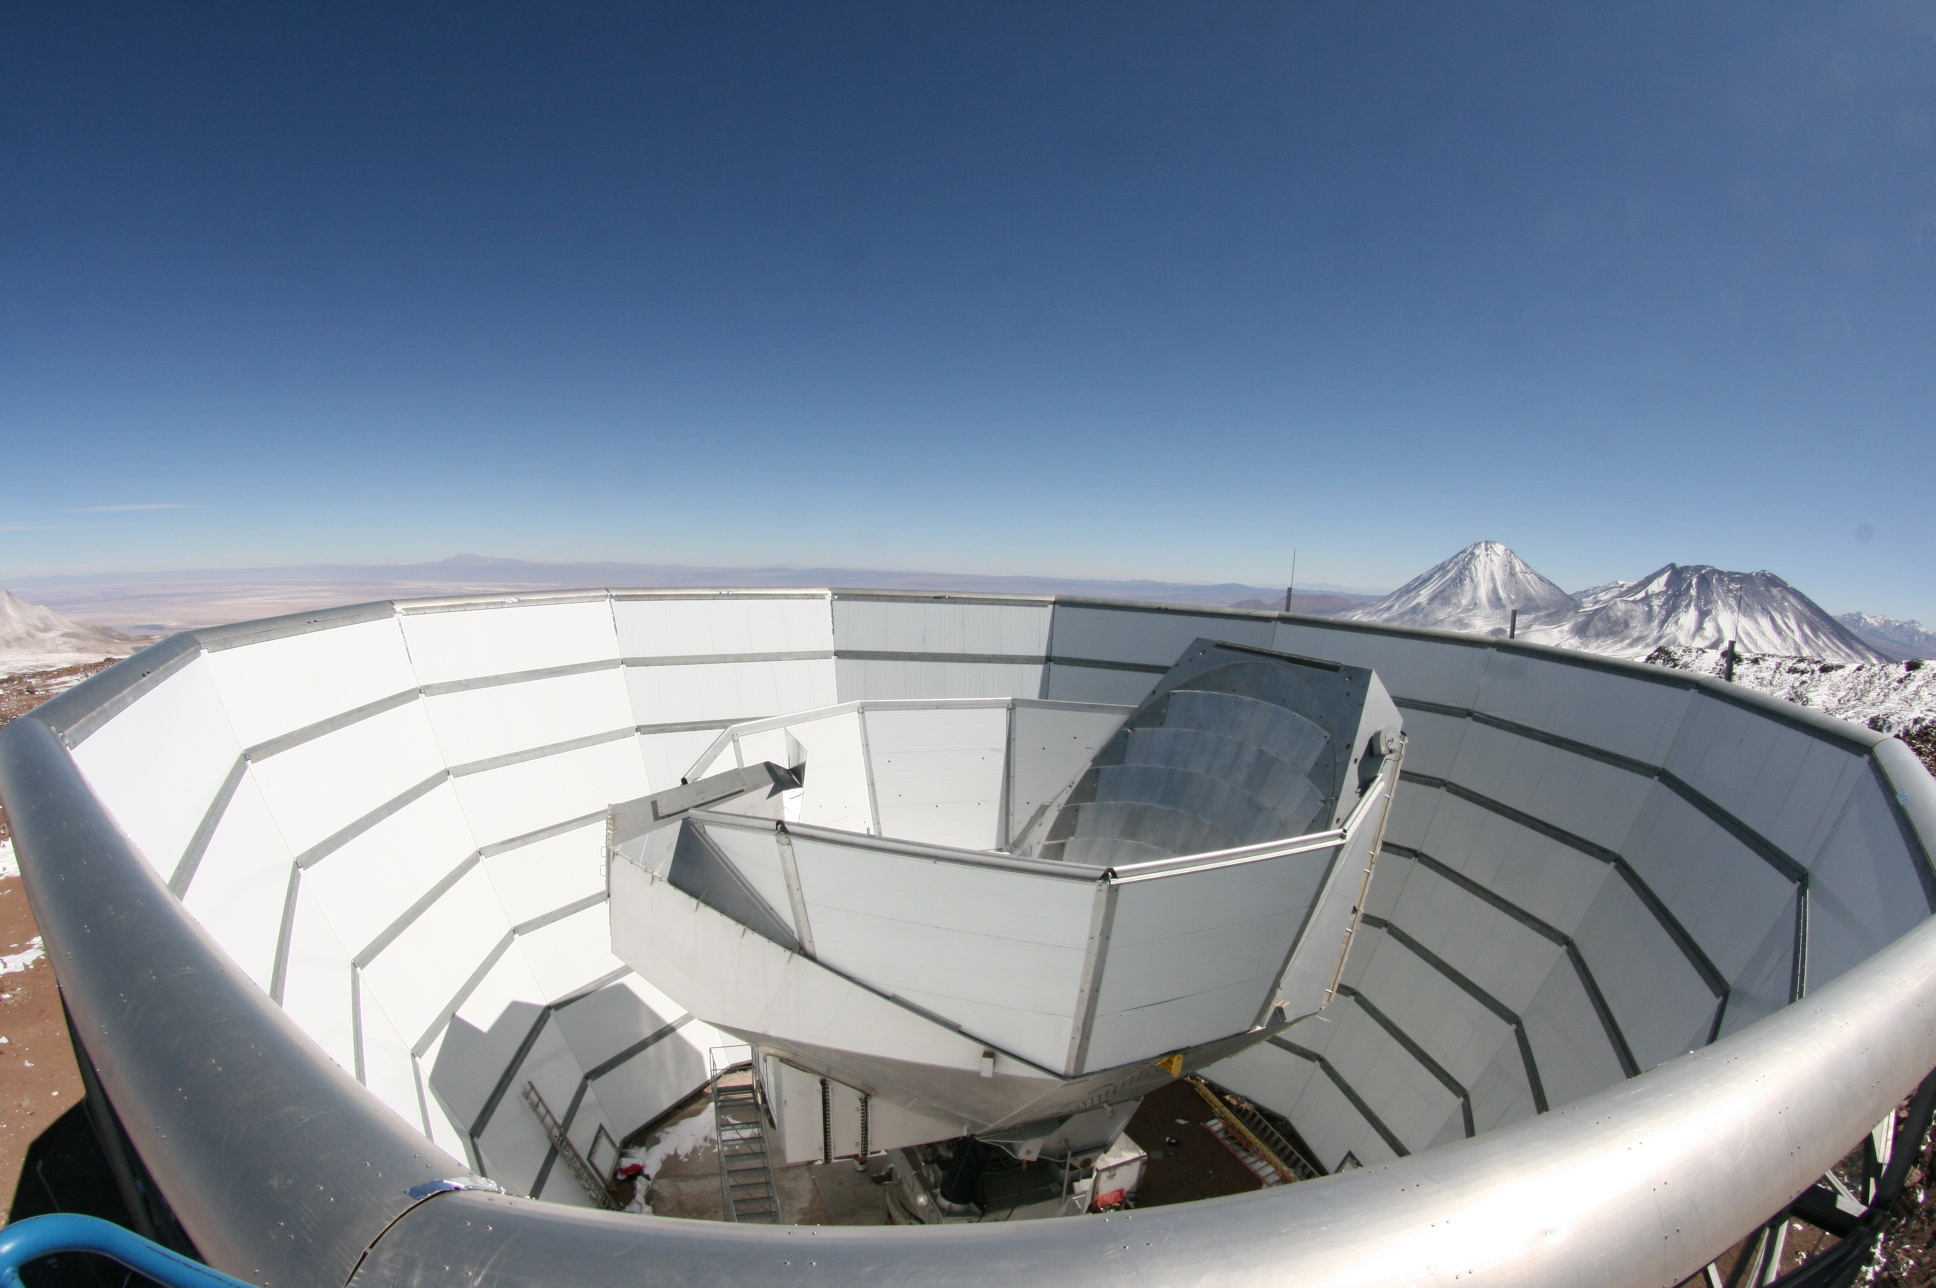
\includegraphics[width = .7\textwidth]{Figures/act_inst_close.jpeg}
    \caption{The Atacama Cosmology Telescope, surrounded by its outer ground screen. The inner co-moving screen further shields the instrument from any stray-light.  One can see the top of the primary mirror behind the co-moving screen.}
    \label{fig:act_site}
\end{figure}

\begin{figure}[t]
    \centering
    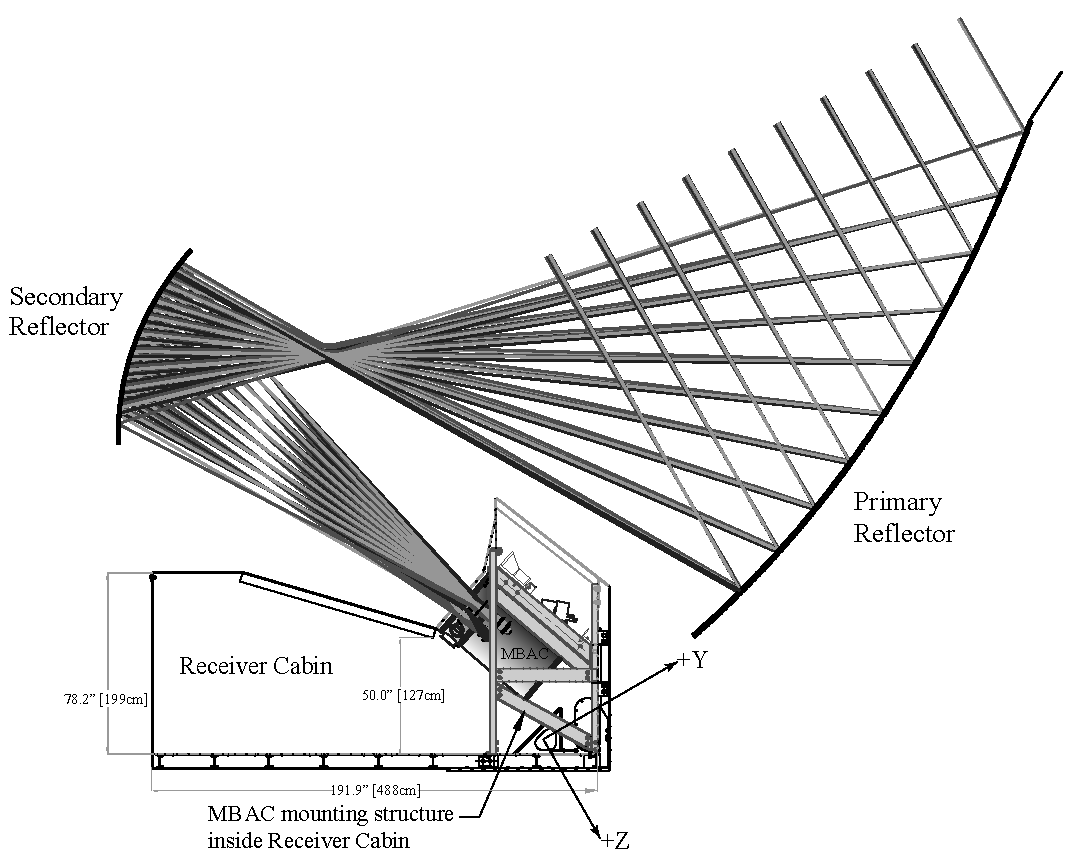
\includegraphics[width = .8\textwidth]{Figures/act_inst.pdf}
    \caption{Ray-trace diagram of the Atacama Cosmology Telescope~\cite{act_inst}.  The telescope is an off-axis Gregorian with two reflectors: the primary is 6\,m in diameter and the secondary 2\,m.  The rays trace into the Millimeter Bolometer Array Camera (MBAC) cryostat which houses the telescope's detectors.}
    \label{fig:act_inst}
\end{figure}

In Chapter~\ref{ch:actbeams} I present the characterization of the ACT beam using point-source stacking.  From the stacking, I also determine polarization leakage in the maps.

\begin{table}[t]
    \centering
    \begin{tabular}{|l|l|l|l|} \hline
        \textbf{ Parameter} &  \textbf{PA4 F150} &  \textbf{PA5 F090}  &  \textbf{PA6 F090}  \\ \hline \hline
        Number of Bolometers & 510 & 510 & 510\\\hline
        Center Frequency (GHz) & 150\,GHz & 90\,GHz & 90\,GHz\\\hline
        Base Temperature & 100\,mK & 100\,mK & 100\,mK\\\hline
        % Angular Resolution & 1 arcmin &1 arcmin &1 arcmin\\\hline
        % Solid Angle & & &\\\hline
        % Sky Coverage & & &\\\hline
    \end{tabular} \caption{ACT Key Characteristics.}
    \label{tab:act}
\end{table}

\section{The Simons Observatory}

SO will test cosmic inflation during the early universe, characterize the primordial perturbations, measure the effective number of relativistic species and the sum of the neutrino masses, and improve our understanding of galaxy evolution and the era of cosmic reionization~\citep{so19,so_science}. 

An ongoing challenge in cosmology instrumentation has been characterizing the polarization spectra of the CMB.  Specifically, the B-mode polarization of the CMB offers a unique window into early-universe physics~\cite{}.  Because scalar perturbations generate E-mode polarization, a measurement of the B-mode polarization directly quantifies the scalar-to-tensor ratio $r$.

The CMB serves as a backlight for large-scale structure, therefore providing insights into gravitational lensing, and ...

The resolution of SO will result in a catalog of extragalactic sources, including active galactic nuclei (AGN), dusty star-forming galaxies, and transient sources including Gamma Ray Burst (GRB) afterglows~\cite{so_science}.  SO expects to catalog 10,000-15,000 AGN sources at flux-densities above 7\,mJy~\cite{Tucci_2011}.  The low frequency coverage of SO will compliment comparison work with other catalogs (e.g. VLA/VLASS, ASKAP/EMU, MeerKAT/MIGHTEE)~\cite{so_science}.  Dusty star-forming galaxies seen by SO will include local galaxies ($z<0.1)$ and high redshift galaxies (approximately $2<z<4$), and strong lensed galaxies beyond this range~\cite{Marrone_2017}.

\begin{figure}[t]
    \centering
    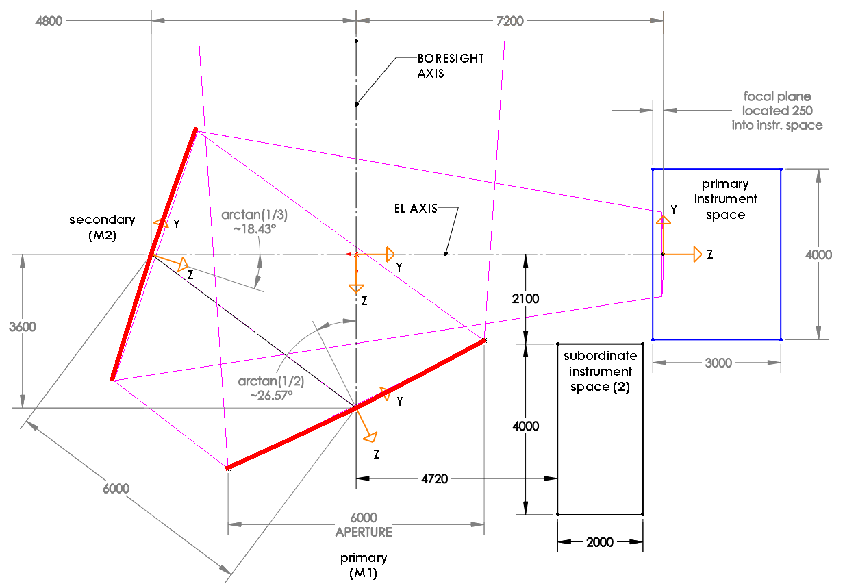
\includegraphics[width = .9\textwidth]{Figures/LAT_rt.pdf}
    \caption{Ray-trace diagram of the Simons Observatory Large Aperture Telescope~\cite{Parshley_2018}.  The telescope is a cross-Dragone with two reflectors, both 6\,m in diameter.  The rays trace into the Large Aperture Telescope Receiver (LATR) cryostat which houses 13 optics tubes.  The optics tubes guide the photons onto the detectors in the focal plane, which are cooled to 100\,mK.}
    \label{fig:so_inst}
\end{figure}

The Simons Observatory (SO) is a series of millimeter-wave telescopes designed to observe the Cosmic Microwave Background (CMB) temperature and polarization signals to an unprecedented sensitivity~\cite{gali18, so19}. With the combination of one Large Aperture Telescope (LAT)~\cite{xu/etal:2020c, zhu18, orlo18, coppi/etal:2018} and three Small Aperture Telescopes (SAT)~\cite{ali20}, the experiment will measure the temperature and polarization anisotropy of the cosmic microwave background with $\sim$\,70,000 background noise limited detectors operating at $\sim$\,100\,mK. 

The Simons Observatory was deployed in the Parque Astronomico located in the Atacama Desert in Chile. The telescope site is situated at an elevation of 5200 meters near the peak of Cerro Toco at $22 ^\circ$ 57' S, $67^\circ$47' W. The arid conditions and elevation at the site minimize contamination to millimeter wave signals from water vapor. 

\begin{table}[ht]
    \centering
    \begin{tabular}{|l|l|l|l|} \hline
        \textbf{ Parameter} &  \textbf{LF} &  \textbf{MF}  &  \textbf{UHF}  \\ \hline \hline
        Number of Bolometers & $>$20,000& $>$20,000& $>$20,000\\\hline
        Base Temperature & 100\,mK & 100\,mK & 100\,mK\\\hline
        Angular Resolution & 1 arcmin &1 arcmin &1 arcmin\\\hline
        Solid Angle & & &\\\hline
        Center Frequency (GHz) & 27-270\,GHz & 27-270\,GHz & 27-270\,GHz\\\hline
    \end{tabular} \caption{SO Key Characteristics.}
    \label{tab:so}
\end{table}

\subsection{Large Aperture Telescope}

The primary mirror is 6\,m in diameter and constructed out of 77 individual adjustable panels, while the secondary mirror is 6\,m in diameter and constructed out of 69 adjustable panels \cite{gali18}.

Figure~\ref{fig:LATR_Cross} shows a cross-section of the LAT Receiver, which houses up to thirteen optics tubes~\cite{Xu_2021}.

Chapter~\ref{ch:ot_holo} presents radio holography measurements of the LAT optics tube, where I characterize the optical performance of the LAT Receiver optics tube.

\subsection{Small Aperture Telescope}

The Small Aperture Telescope (SAT) optical design is a 0.42\,m diameter refractive telescope.  Three SATs will measure the largest angular scales visible from the Atacama Desert.

In Chapter~\ref{ch:sat_holo}, I present radio holography measurements of the SAT optics tube.
\chapter{Metamaterial Microwave Absorber (MMA) and its Cryogenic Applications}
\label{ch:mma}
The following was published in Applied Optics in 2021~\cite{Xu_2021}.  The paper was selected as Editor's Pick and given a press release here~\cite{MMApress}.

\section{Introduction}
Modern ground-based millimeter-wave telescope receivers have advanced to the point where detector noise is dominated by photon noise, meaning the thermal or electronic noise intrinsic to the detectors (and the associated readout system) is less than the photon noise from the incident light. The in-band optical power incident on the detectors---closely related to the photon noise---arises from the sky signal, the atmosphere, and stray light outside the desired optical path. The out-of-band instrument spectral and angle response is largely set by filter stack and baffle implementation.

\begin{figure*}
    \centering
    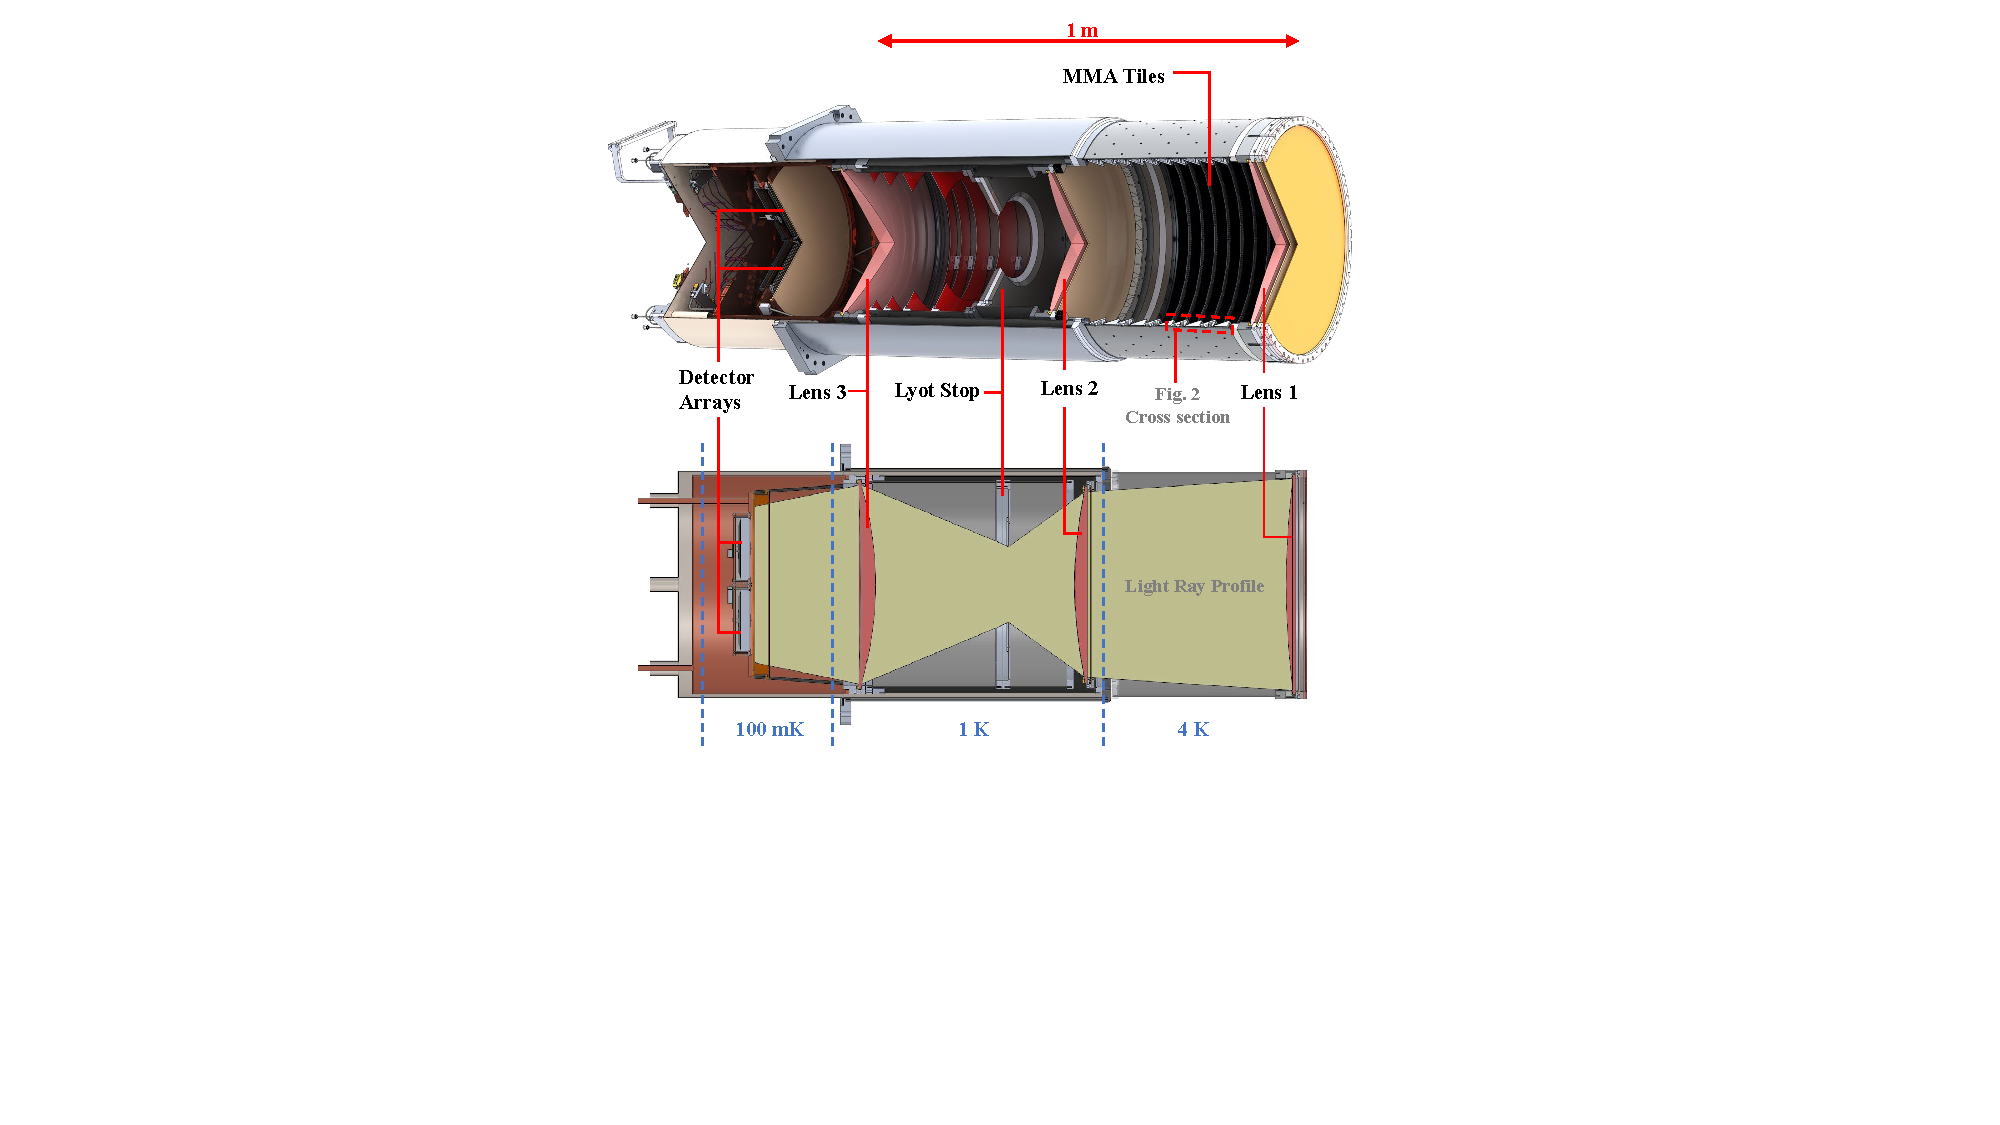
\includegraphics[width = .9\textwidth]{Figures/latr_ot.pdf}
    \caption{Large Aperture Telescope Receiver (LATR) optics tube in the Simons Observatory. A detailed rendering of the optics tube design is shown in the upper part, and a simplified schematic cross-section is shown in the bottom part. Incoming light enters the optics tube from the right and focuses on the detector arrays on the left via three lenses. The yellow-shaded region in the bottom part shows the geometric light ray profile. Operational temperatures for different parts of the optics tube are also annotated. More details of the optics tubes are described in~\cite{xu/etal:2020c}. The MMA tiles are installed in the regions between lens\,1 and lens\,2 at 4\,K. Fig.~\ref{fig:tile_design} shows a cross-section of the MMA tile assembly (box with red dashed lines) in the optics tube and the detailed design of one tile. A flat version of the MMA tile (Section~\ref{sec:future_applications}) was also used to cover the front and back of the Lyot stop at 1\,K.}
    \label{fig:latr_ot}
\end{figure*}

The sky signal and the atmosphere power loading observed by the detectors cannot be reduced by improving the instrument, whereas the stray light loading can be reduced by a more effective design. Instead of following the main optical path, stray light is reflected or scattered by the side walls of cryogenic receivers before being absorbed by the detectors. Therefore, stray light can not only compromise image fidelity through ghosting or glint, but also degrades the detector sensitivity. This chapter concentrates on suppressing stray light by minimizing reflection and scattering within cryogenic receivers~\cite{iuliano/etal:2018, thornton_2016, sharp/etal:2008}.

Terminating stray light at the lowest possible temperature is typically achieved by cryogenic baffling design, which minimizes reflection and scattering.  Ideally, the baffling surfaces are constructed of millimeter-wave absorbing material, with high absorptivity and low reflection/scattering over a wide range of incident angles and frequencies. Beyond the required optical properties, the absorbers should be efficiently cooled to cryogenic temperatures with robust thermal contacts and be able to withstand the mechanical stress associated with thermal cycling. Since cryogenic space is scarce, the absorbing material is often required to be as compact as possible. Ideally, the absorber should be light in mass, especially for future space missions.

Available options include conductively-loaded-epoxy~\citep{Wollack2008}, and commercially-available absorptive sheets\footnote{For example, HR-10 sheets from Emerson\,\&\,Cummings.}/tiles\footnote{For example, Tessellating Terahertz Radar Absorbing Materials (RAM), Thomas Keating Ltd.}. The conductively-loaded-epoxy relies on the conductive materials to absorb the radiation; however, the high index of refraction of the epoxy gives high reflectance and scattering, depending on the roughness of the surface. In addition, the epoxy normally has a $>$\,2\,g$\cdot$cm$^3$ density, adding a significant mass to the cryogenic system. The commercially-available absorptive sheets and tiles provide high absorption, while mechanically and cryogenically attaching them to low-temperature surfaces poses great challenges. Recent development on 3D printing also enables more absorber designs~\cite{petroff/etal:2019}, while mass production at low cost is still a challenge. To overcome these obstacles, the SO team developed injection-molded tiles with a metamaterial gradient index anti-reflection coating. Metamaterials are artificially engineered materials, in terms of content and geometry, to achieve physical properties that are not available in nature~\cite{wollack/etal:2016, ding/etal:2012, watts/liu/padilla:2012}. Our solution provides high absorption with customized thermal and mechanical interface for cryogenic applications. 

Here I describe the design (Section~\ref{sec:optical_design}) and characterization (Section~\ref{sec:optical_testing}) of the tiles, along with its application within the Simons Observatory (SO) Large Aperture Telescope Receiver (LATR)~\cite{zhu18, orlo18} and Small Aperture Telescopes (SAT)~\cite{ali20}.\footnote{The MMA tiles are also used in CCAT-Prime cam~\cite{vavgiakis/etal:2018}.}  I also discuss potential future applications in Section~\ref{sec:future_applications}.

\begin{figure*}[t]
    \centering
    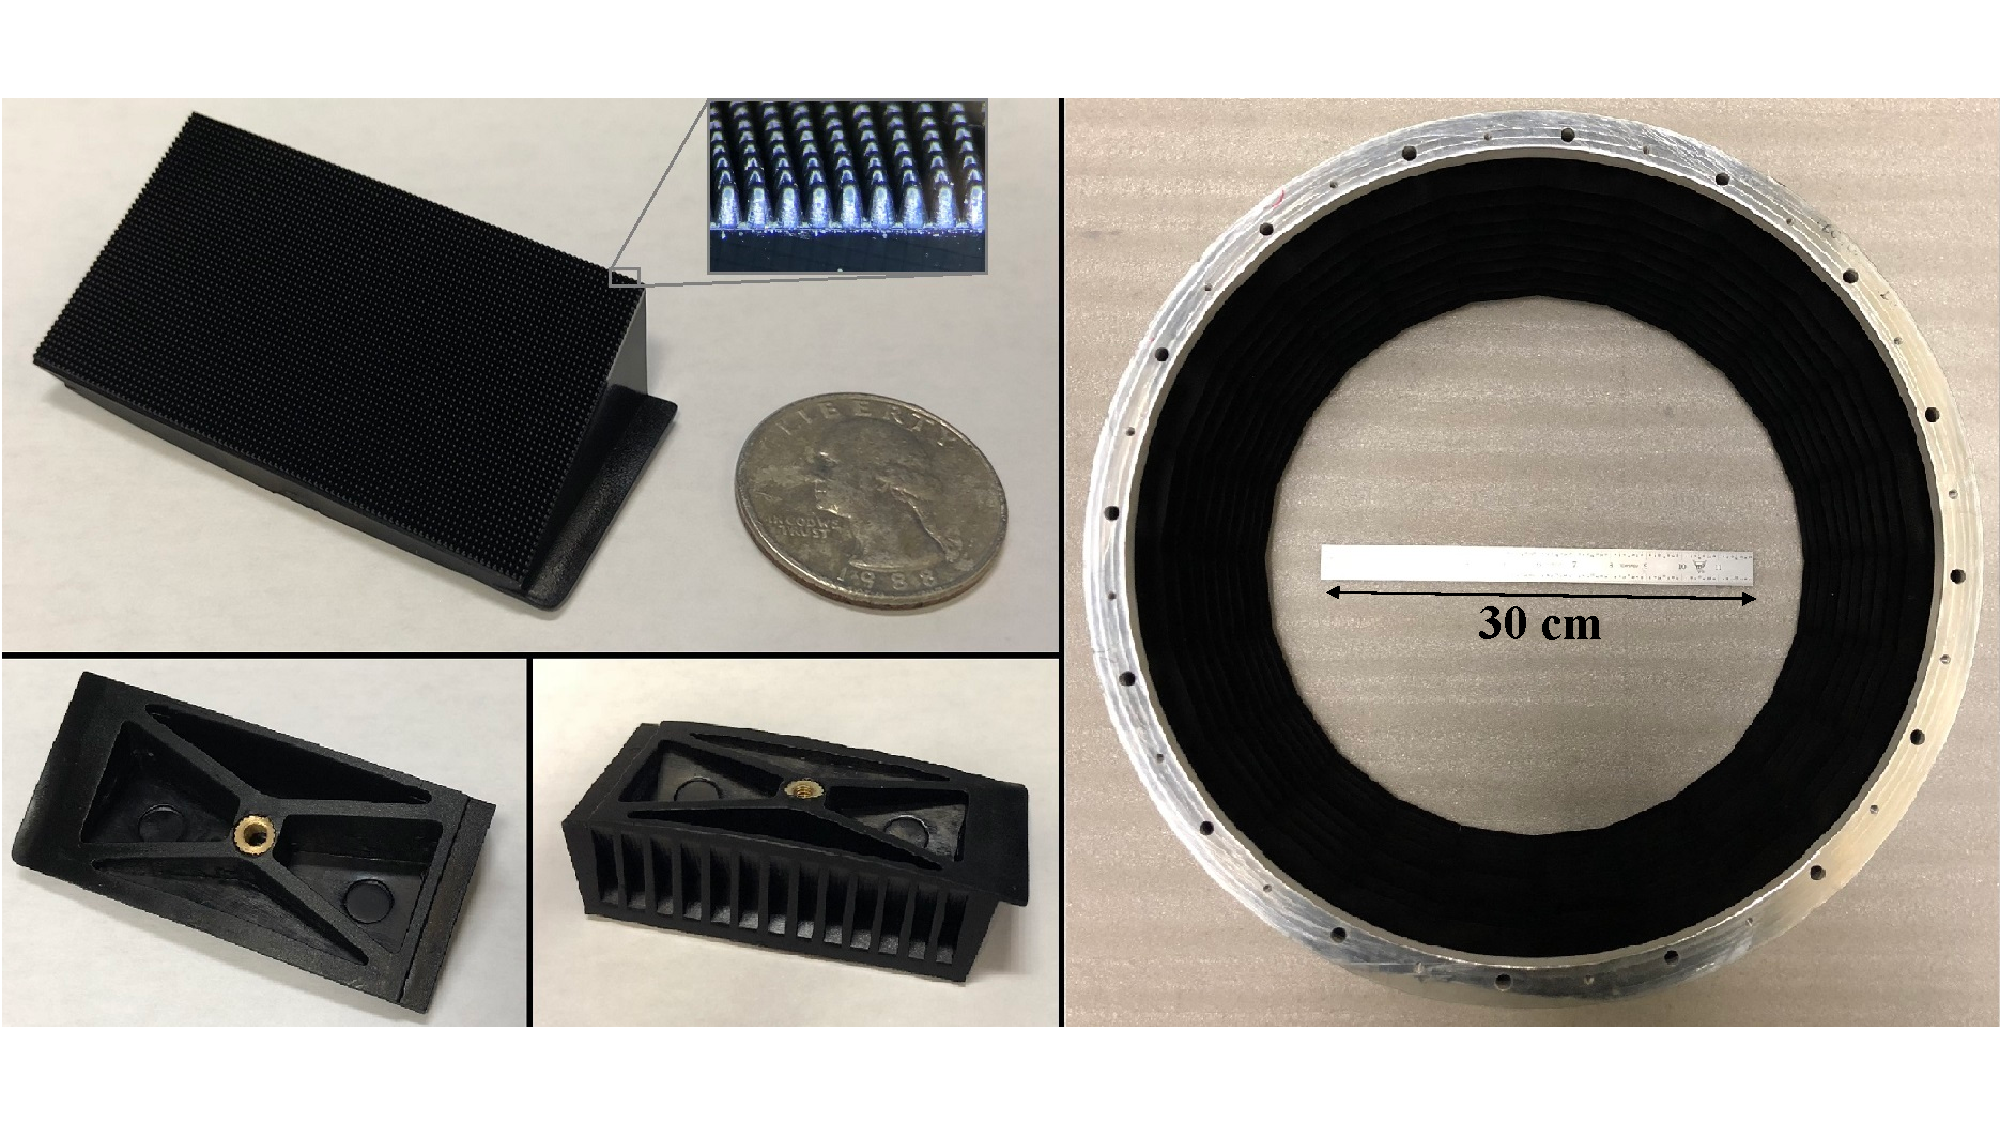
\includegraphics[width = \textwidth]{Figures/real_tile.pdf}
    \caption{Manufactured MMA tiles. The manufactured tiles are presented from different perspectives. The top left photo shows one tile from the absorbing surface. A microscope photo of the pyramids is shown in the insert. The pitch between pyramids is kept as 0.6\,mm as designed. The bottom left two photos show the back of the tile from two other perspectives. The light weighting pockets are visible along with the brass injected M3 nut for fastening. The photo on the right shows the assembly of 240 tiles installed on the wall of the optics tube section (see Fig.~\ref{fig:latr_ot}). A ruler ($\sim$\,30\,cm) is placed in the center for scale. Note that the absorbing surface appears to be black and featureless in the assembly photo. The condition stays the same regardless of lighting in the room, which supports the effectiveness of the AR-coating design even in optical.}
    \label{fig:real_tile}
\end{figure*}
\section{Optical Design}
\label{sec:optical_design}

The ideal baffling material minimizes reflection and scattering of light over the relevant range of angles of incidence, while mechanically (and even cryogenically) fitting within optical systems.  In the case of the SO LATR~\cite{xu/etal:2020c, zhu18, orlo18, coppi/etal:2018}, the desire to close-pack the optics tubes limits the radial extent of the absorbing material to about 1\,cm to avoid clipping the beam near the front of the optics tubes (between Lens\,1 and Lens\,2 in Fig.~\ref{fig:latr_ot}).



A detailed study of the SO LATR optics tubes revealed that improving light absorption near the front of the optics tubes would most significantly reduce optical power loading~\cite{Gudmundsson:21}. This study also showed that stray light on that section of the optics tubes ranges from $55^\circ$ to $90^\circ$ relative to the surface normal, taking up $\sim$\,2\,\% of the solid angle. Controlling the stray light in that section improves the telescope's mapping speed by 40\,--\,80\%,\footnote{Mapping speed is defined as $1/\textrm{NET}^2$, where NET is the noise-equivalent-temperature (NET). More details about mapping speed are available in \cite{hill/etal:2018}.} significantly increasing the sensitivity of the instrument. The Fresnel Equations show that the reflectance for dielectric materials approaches unity near grazing angles.  To improve performance at these high angles, the absorbers were fabricated with the absorbing surface tilted at $26^\circ$ relative to the normal of the optics tube surface (Fig.~\ref{fig:tile_design}). The tilting reduces the angle of incidence by 26\dg{} to $<64^\circ$ (incoming light cannot exceed 90\dg{} angle of incidence) where the absorbing surface provides desired optical performance. Note that the angle of incidence is viewed in a time-reverse fashion here.

The goal of mass production led to the selection of injection molding carbon-loaded plastics. The carbon content increases the optical loss of the plastic materials so that the radiation is sufficiently attenuated within a small depth of bulk materials. However, the carbon-loaded plastics have relatively high dielectric functions, leading to high reflectance on a flat surface. Therefore, an effective anti-reflection coating is designed.  The full design and thermal testing is described in~\cite{Xu_2021}.

\begin{figure*}[t]
    \centering
    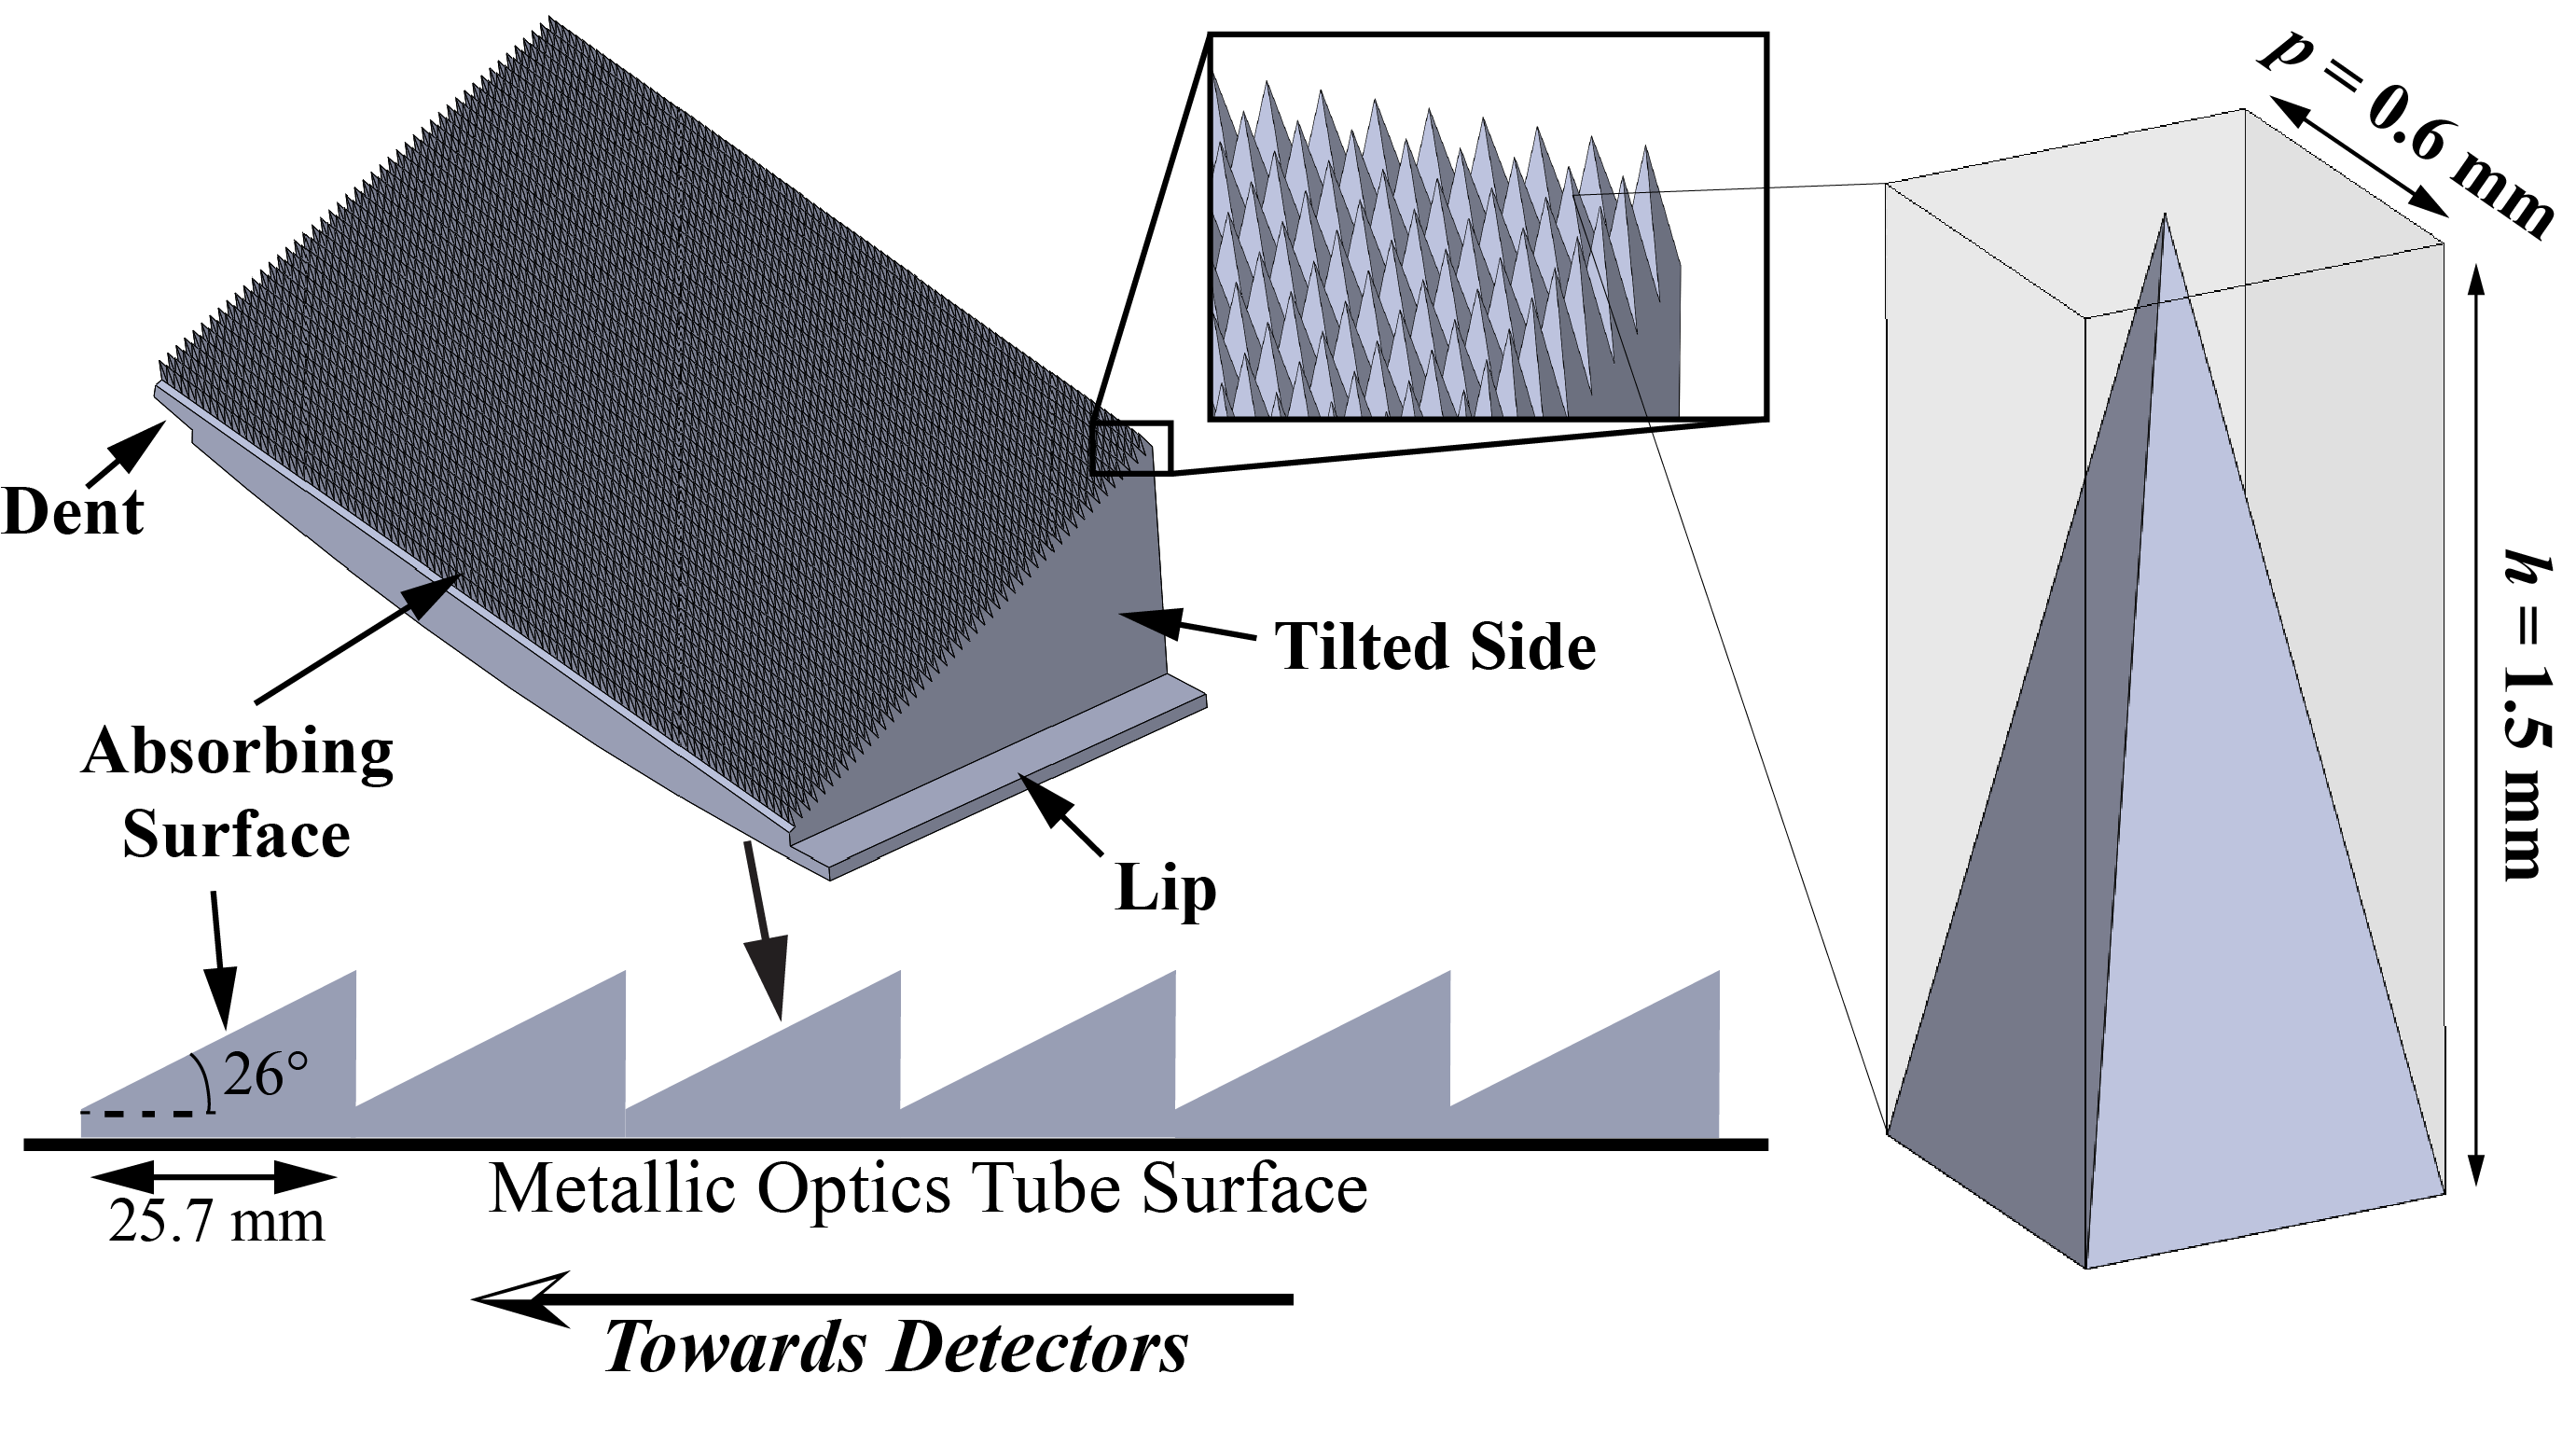
\includegraphics[width = .9\textwidth]{Figures/tile_design.png}
    \caption{MMA tile design. A snapshot of a single tile design is shown. The tilted upper surface has the pyramidal structures as described in Section~\ref{sec:optical_design}. A zoom-in plot shows details of the pyramidal structures, acting as a metamaterial anti-reflection coating. Another insert on the right zooms in further and shows one single unit of the metamaterial structure, with a pitch, $p =0.6\,$mm and a height, $h = 1.5\,$mm. The tile bottom is curved to fit the cylindrical inside surface of the metallic optics tube, which is used for structural support, heat sinking, and reflective optical termination for the absorptive tiles. A lip and a dent are for seamless tessellating. A cross-section of the segmented tilted surface is shown in the lower left part. In a time-reverse fashion, light rays coming from the left would hit the tilted surface with a $<$\,$64^{\circ}$ angles of incidence, where the absorbing surface achieves the desired optical performance.}
    \label{fig:tile_design}
\end{figure*}

\section{Optical Testing}
\label{sec:optical_testing}

Optical properties of the MMA tiles were measured for diffuse reflection, or scattering, at 110\,GHz and specular reflection in the frequency range from 90\,GHz to 170\,GHz. The measurements also covered different angles of incidence. The results verified that the tiles achieved the designed high absorptivity and low reflection and scattering.

The optical measurements were conducted at room temperature. A consideration in using the technology at low temperatures is the following---the detailed composition and realization of the material (e.g., amorphous lamp black, activated carbon, pyrolytic carbon, graphite, etc.) influences the temperature dependence of the bulk resistivity and thus the dielectric function of the plastic \cite{Smith1956,Sihvola2008}. From the measurement of the bulk resistivity at 3\,K relative to ambient, this is a modest effect for the carbon loaded TPU formulation explored here. The design of the MMA tiles is insensitive to the dielectric function of the bulk dielectric mixture. Therefore, dramatic changes of the tile's optical properties are not expected in cryogenic temperatures down to 3\,K or lower. 

\begin{figure*}[t]
    \centering
    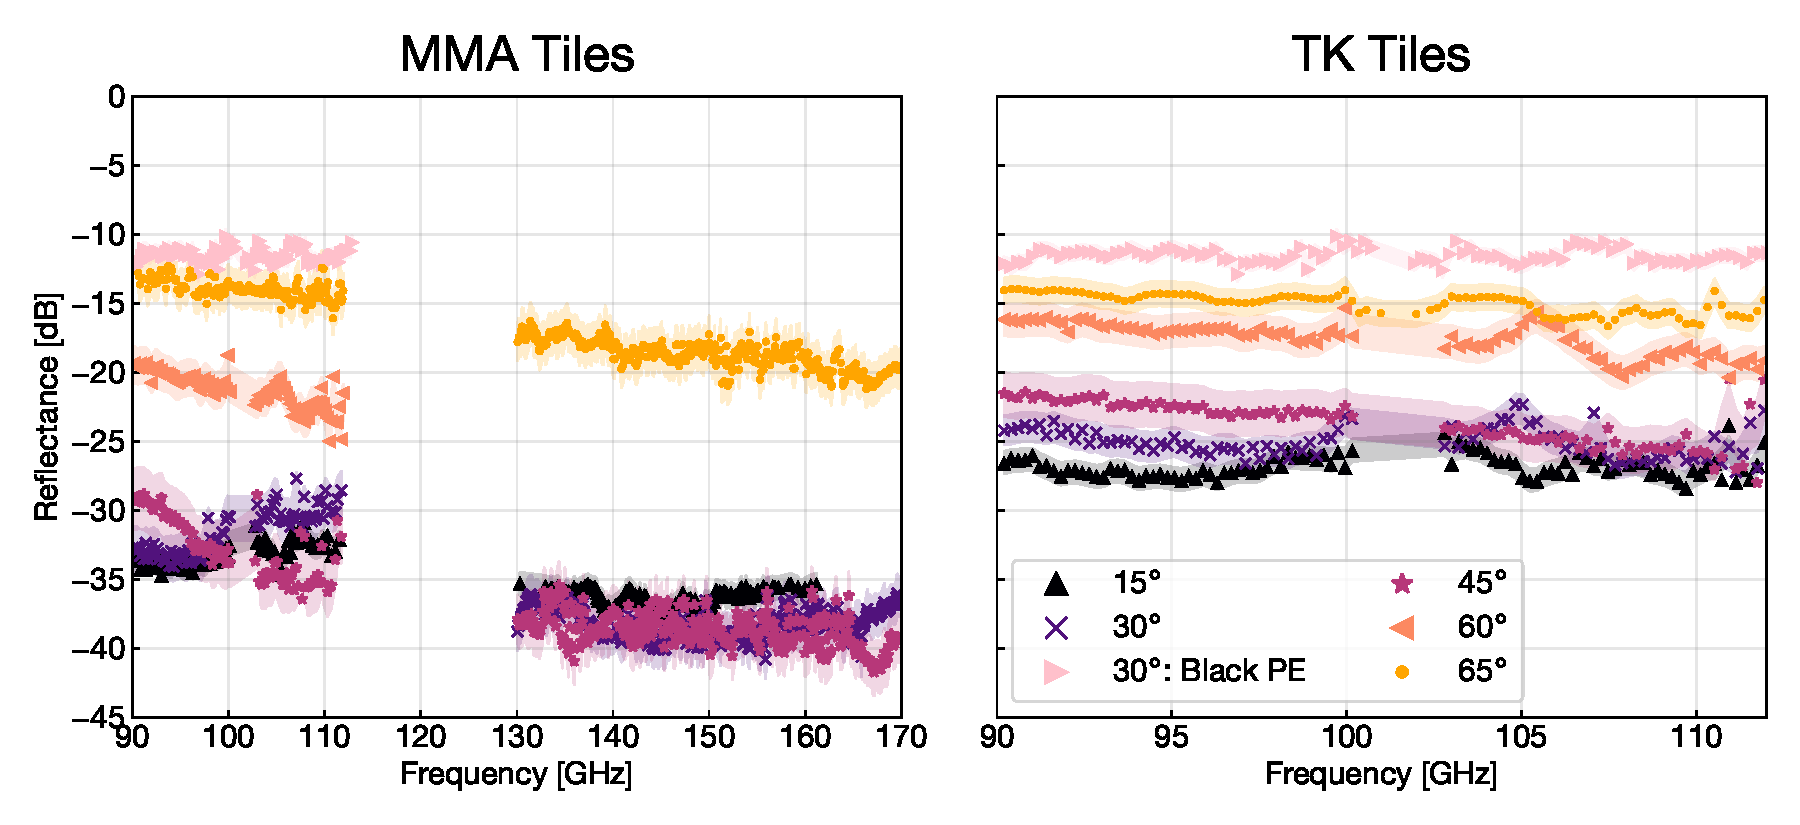
\includegraphics[width = \textwidth]{Figures/refl_2.2020.pdf}
    \caption{Specular reflectance measurements. The two panels show the specular reflectance measurements of the MMA tiles and the TK tiles at different angles of incidence, including $15^{\circ}$, $30^{\circ}$, $45^{\circ}$, $60^{\circ}$, and $65^{\circ}$. The samples are measured in W-band (90\,GHz to 110\,GHZ) and D-band (130\,GHz to 170\,GHz). The left panel shows the W-band (90\,GHz to 110\,GHZ) and D-band (130\,GHz to 170\,GHz) reflectance of the MMA tiles. The measurement gap in the left panel is due to the different frequency bands of the two sources used in the setup. The right panel measures the W-band (90\,GHz to 110\,GHZ) reflectance of the TK tiles. The two panels share the same y scale for comparison. The measurement of a flat black polyethylene sample without a AR-coating is included in both panels, which is conducted with a $30^{\circ}$ angle of incidence. Comparing the sample without an AR-coating (purple triangles) and the MMA tiles (blue crosses), $\sim$\,$-20$\,dB specular reflectance reduction is achieved with the metamaterial AR-coating.}
    \label{fig:reflection_result}
\end{figure*}


\subsection{Optical Hardware}
\begin{figure}
    \centering
    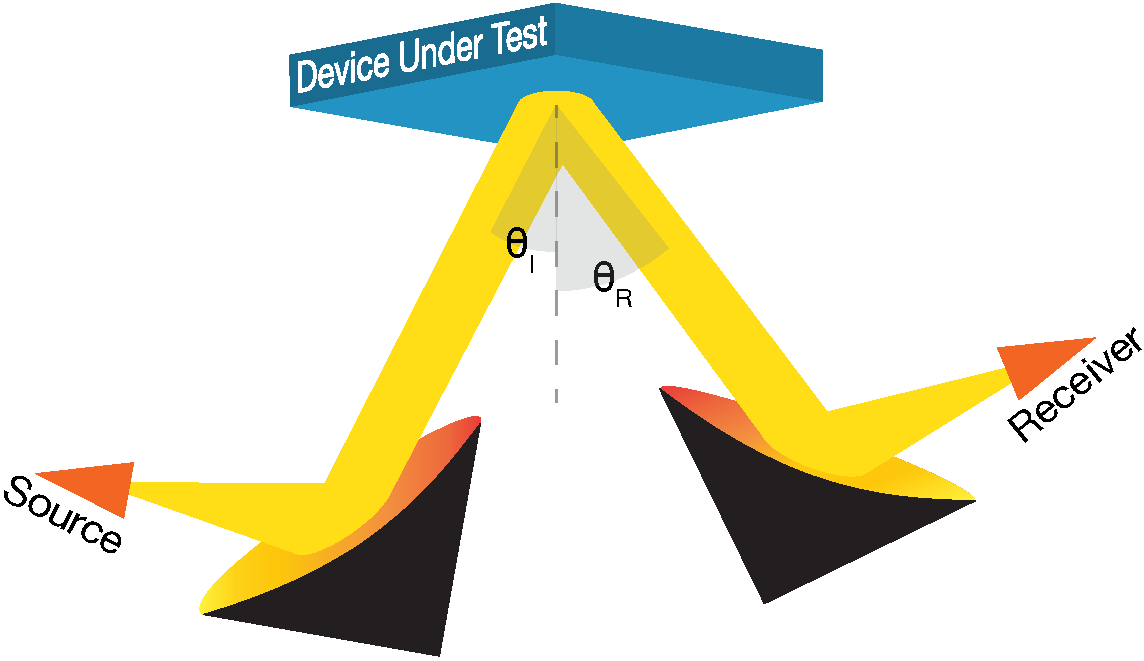
\includegraphics[width = .7\textwidth]{Figures/refl_setup.pdf}
    \caption{Optical measurement setup sketch. The orange lines represent the beam as it travels from the source feed-horn, collimated off of the first mirror and to the sample. After being reflected/scattered by the second mirror, the beam is focused into the receiver to be measured. Incident ($\theta_i$) and receiver ($\theta_r$) angles are controlled by a motor for measuring different angles of incidence and scattered power.}
    \label{fig:optical_setup}
\end{figure}

In the measurement setup, a source emits a millimeter-wave through a feed-horn toward a parabolic mirror, which then reflects a plane wave toward the sample, at an angle of incidence controlled by a rotary stage. The signal reflected off the sample propagates to a second mirror, followed by the receiver feed-horn~\cite{ches18}. The sketch of the setup is shown in Fig. \ref{fig:optical_setup}. Eccosorb HR-10 sheets are placed on surrounding surfaces to reject multipath propagation. The alignment of the receiver is controlled with a three-axis stage. The tilt of the sample is controlled with a three-point micrometer mount.

\begin{figure}[t]
    \centering
    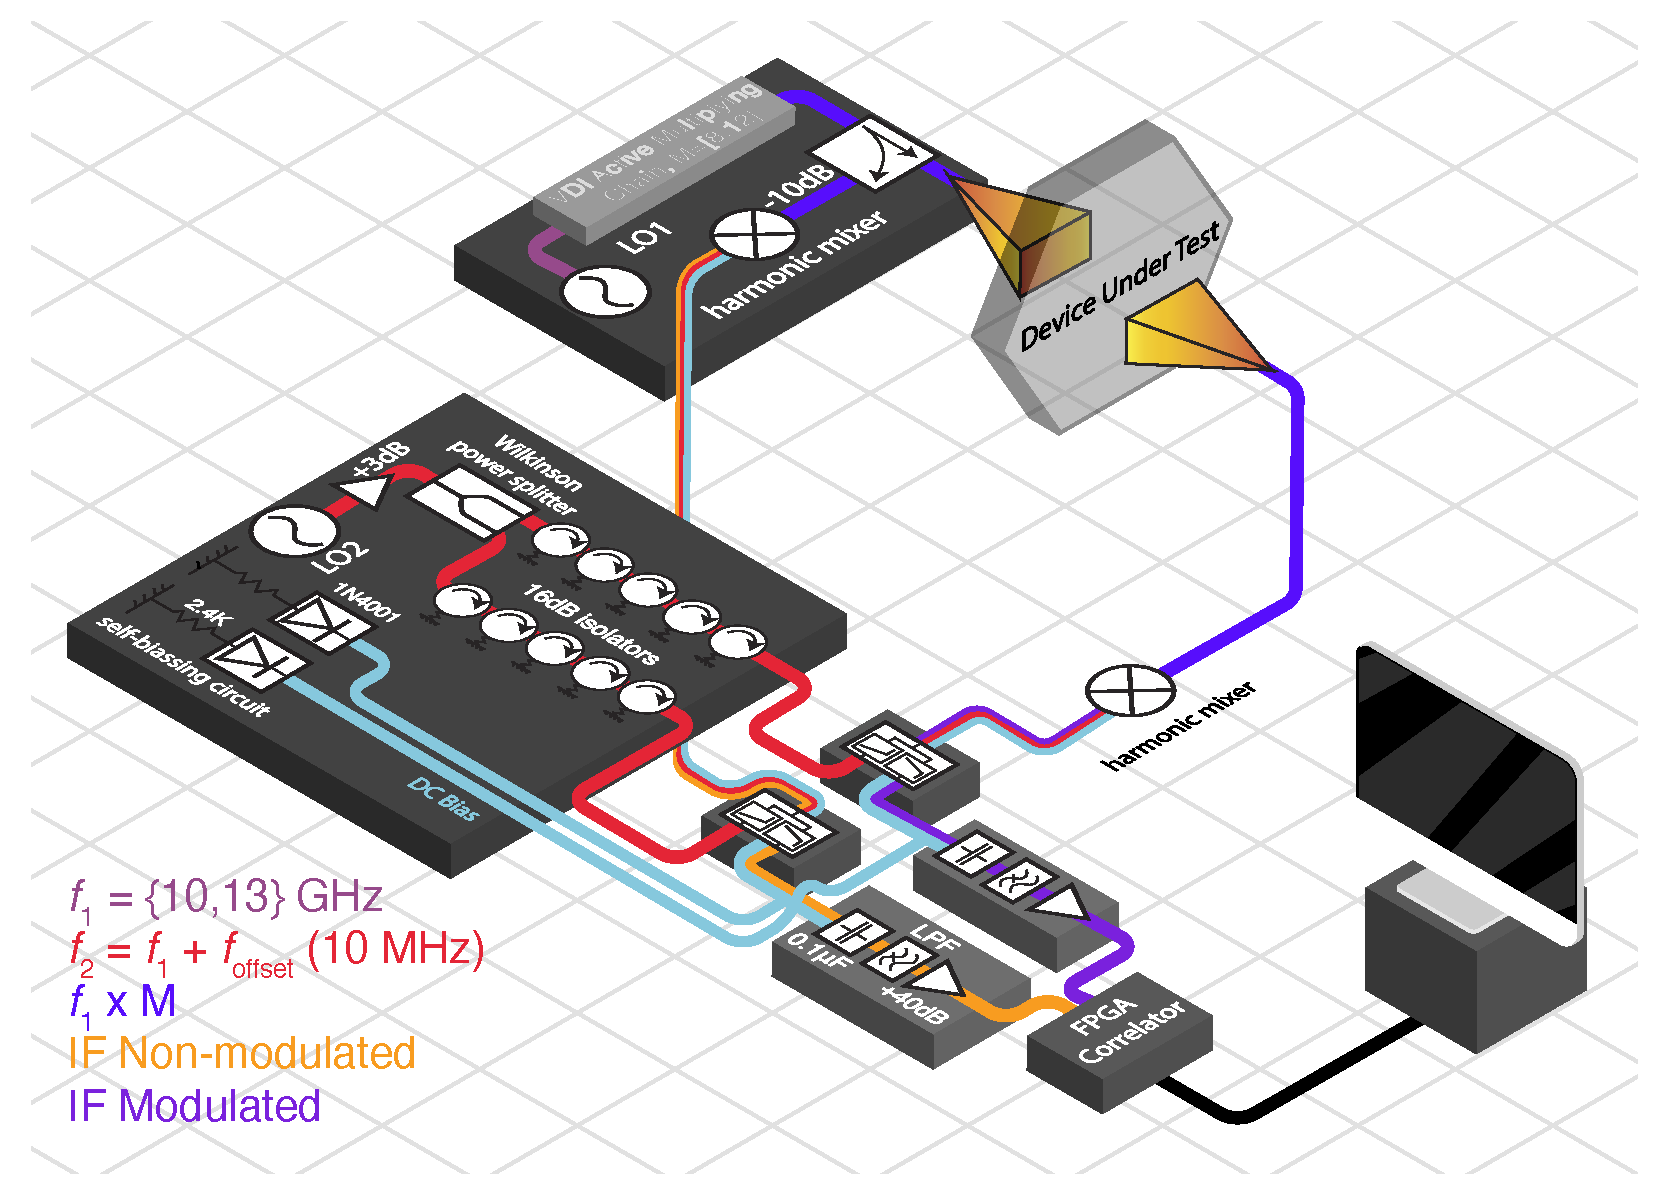
\includegraphics[width = \textwidth]{Figures/refl_isometric.pdf}
    \caption{The correlation receiver setup diagram. A splitter sends one signal from a millimeter-wave source to a Pacific Millimeter harmonic mixer, while sending the same signal to be modulated by the device under test. The reference and modulated signal are mixed with an LO with an offset frequency $f_{\textrm{offset}}$ from the millimeter wave source. The two Pacific Millimeter harmonic mixers extract interference information caused by $f_{\textrm{offset}}$ and sends this to the ROACH-2 field programmable gate array (FPGA) board where the two signals are correlated.}
    \label{fig:holog_ref_setup}
\end{figure}

\subsection{Receiver Electronics}

A correlation receiver is used for these measurements. The receiver compares a reference tone to a signal which has passed through the optical path, creating an interference pattern between the two~\cite{ches18}. The correlation receiver is summarized in Fig.~\ref{fig:holog_ref_setup}.  The Re-configurable Open Architecture Computing Hardware (ROACH-2) board correlates the reference and modulated signals~\cite{roach2}.

The millimeter-wave source sends a signal, ranging from 10.5\,GHz to \,13 GHz, to a multiplier which passes through a passive multiplying chain. The W-band (90\,--\,110\,GHz) and D-band (130\,--\,180\,GHz) millimeter-wave sources use multiplication factors of 9 and 12, respectively. The signal is then modulated by the sample. The modulated and the reference signals are separately sent to two harmonic mixers. The mixers extract interference information caused by the offset frequency and send it to the correlation device. This receiver outputs the amplitude and phase of the signal in narrow (50 MHz) spectral bands.  Only the amplitude is used in this analysis, though I note that the phase information could be used to improve these measurements in the future.

\subsection{Measurement}

In order to measure their optical properties, an array of tiles are screwed down to a 3D-printed plate. The 3D-printed plate compensates the wedge shape of individual tiles so that absorbing surfaces of all tiles are aligned and oriented upward, forming a 30.5$\times$30.5\,cm flat surface (Fig.~\ref{fig:front_tiles}).

For comparison, we acquired the Tessellating Terahertz RAM from TK Instruments.  The TK tiles are 25\,mm $\times$ 25\,mm square tiles that can be tessellated to cover a flat surface. The pyramidal structures ($\sim$2.5\,mm in pitch and height) on the optical surface are designed to reduce the specular reflection and scattering in the 100\,--\,1000\,GHz region. 

\begin{figure}
    \centering
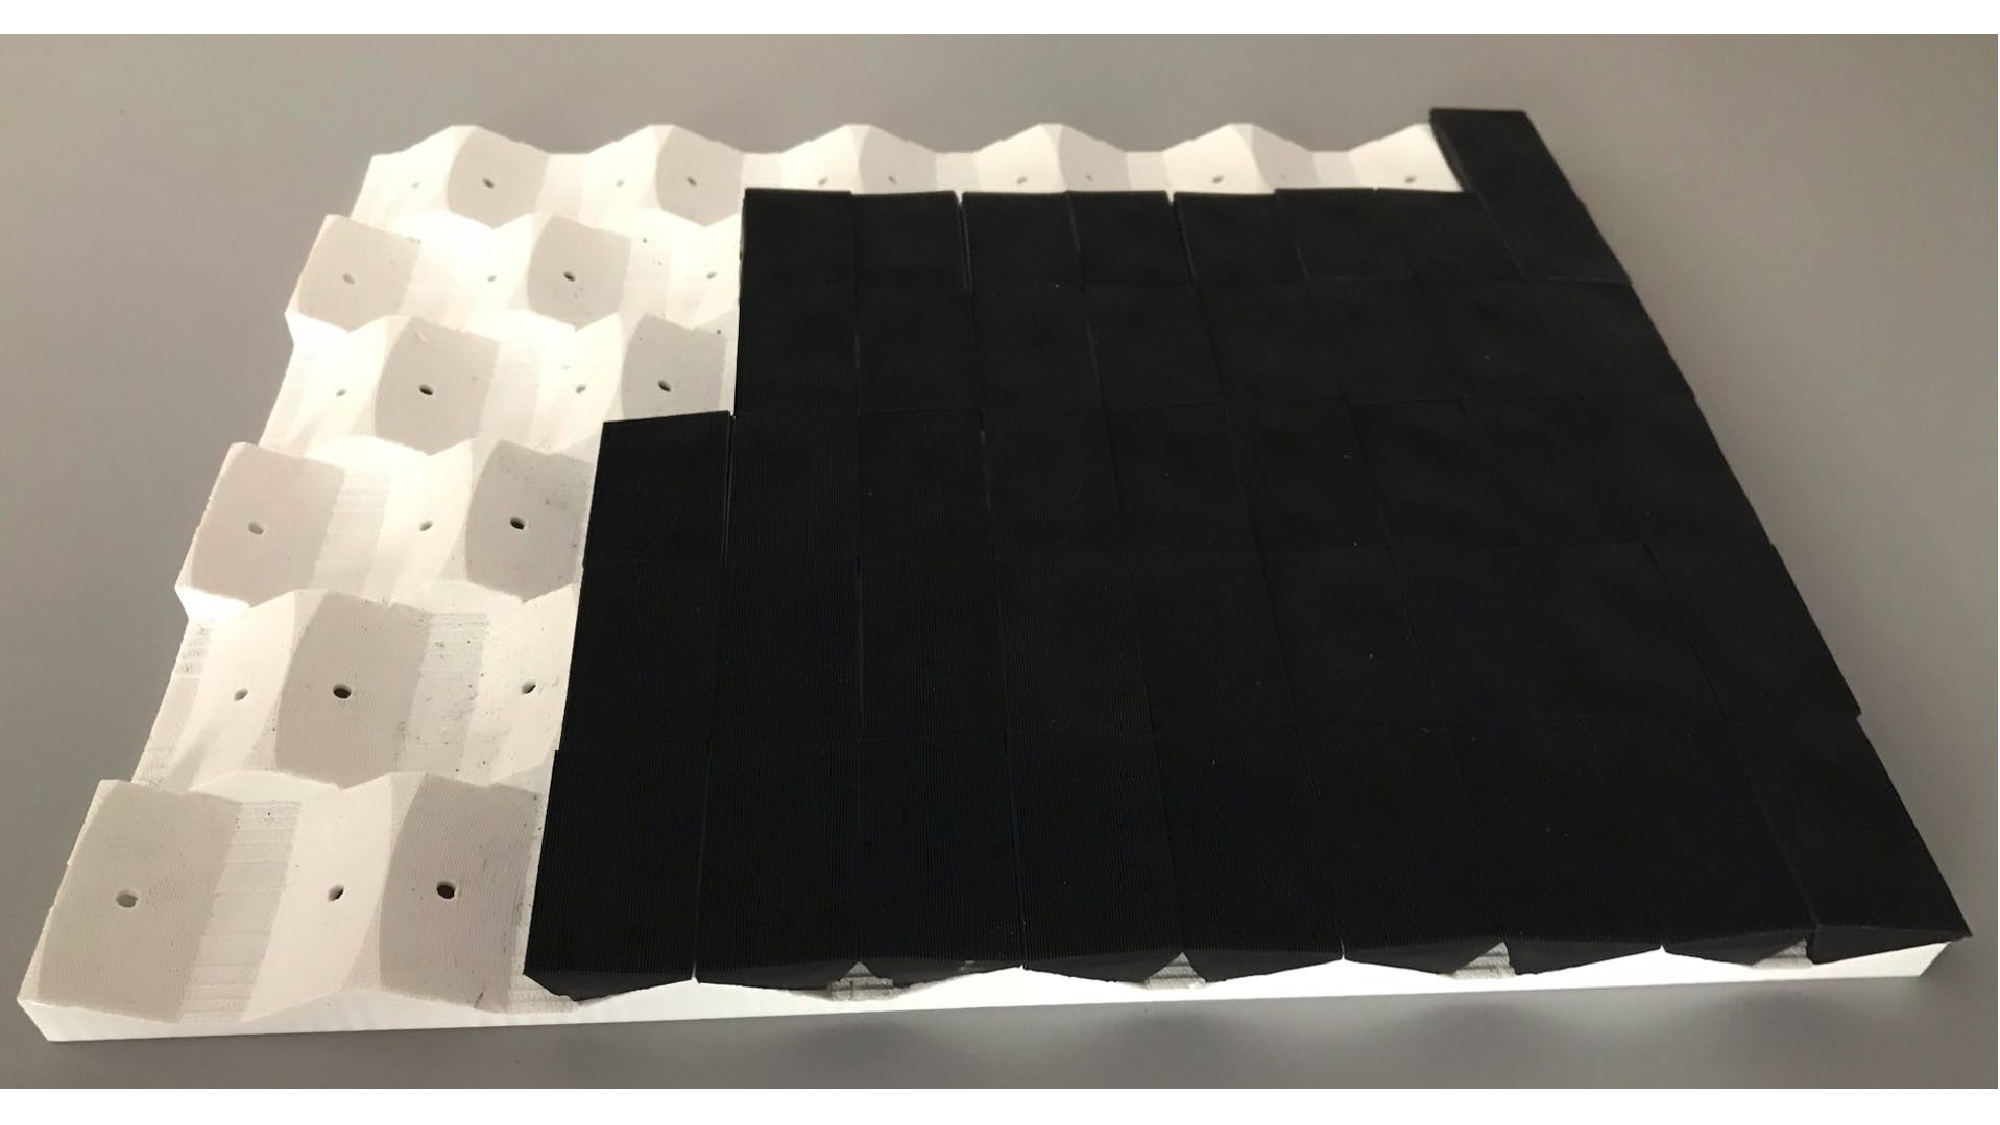
\includegraphics[width = \textwidth]{Figures/flat_sample.pdf}
    \caption{MMA measurement sample. MMA tiles are individually bolted into a 3D-printed plate such that each absorbing surface sits flat to form a 30.5$\times$30.5\,cm testing surface.}
    \label{fig:front_tiles}
\end{figure}

Although the TK tiles and the MMA tiles both have pyramidal structures on the optical surface, they function differently. Pyramids in the MMA tiles, with the sub-wavelength scale, act more as a layer of medium with changing index of refraction; while pyramids in the TK tiles works more within the geometric optics regime to increase the number of bounces of the incoming radiation, due to the adopted surface geometry~\cite{Chuss2017}. The TK tiles have long been the preferred absorbers in millimeter wavelengths due to their optical performance. The measurement of the TK tiles ($\geq$\,200\,GHz) are available in the product website and published literature~\cite{Saily/etal:2004}. Because the MMA tiles are optimized to perform well at the operating wavelengths, an improvement in performance is expected. Even though the measurement only verifies the performance within 90\,--\,170\,GHz, the MMA tiles are designed to work from 90\,--\,270\,GHz following the same physical principles.
\section{Reflection Measurement}

Once the setup is aligned using an aluminum plate in place of the sample, a calibration data set is taken by measuring the specular reflectance of the same aluminum plate as a function of frequency. The sample measurements are then normalized using the aluminum plate data. 

Fig.~\ref{fig:reflection_result} shows the reflected power measured for the MMA and TK samples, with the MMA tiles measured from 90\,GHz to 170\,GHz and the TK tiles measured from 90\,GHz to 110\,GHz. The measured results demonstrate the relative performance of the two. For the MMA tiles, specular reflection is at sub-percent levels ($<$-20 dB) for all angles of incidence except for $65^{\circ}$ ($\sim$\,-15\,dB). Note that $65^{\circ}$ is higher than the angle of incidence upper limit in the SO optical design (see Section~\ref{sec:optical_design}). To demonstrate the effectiveness of the anti-reflection coating, a flat carbon-loaded polyethylene (PE) sample without an AR-coating was measured. During the test, a proper flat molding material sample was not available. Therefore, I measured the carbon-black loaded PE sample---with a lower dielectric function---as a lower limit of the reflectance from a flat molding material sample. With the coating, the MMA tiles reduce the specular reflection by $\sim$\,$-20$\,dB. Meanwhile, the specular reflection from the TK tiles is 5--10\,dB higher than that from the MMA tiles at different angles of incidence.


\section{Scattering Measurement}

The scattered power off the surface of the sample is determined by measuring the received power as a function of the receiver's angle, fixing the source feed horn at a set angle (Fig. \ref{fig:optical_setup}). The source (incident) and receiver (scattered) angles are controlled by two rotary stages. The radiative source sends one frequency and is held at a constant position (i.e. angle of incidence), while the receiver sweeps across different angles. Fig.~\ref{fig:scatter} shows the scattering measurement with a 110\,GHz source at four angles of incidence: 15$^{\circ}$, 30$^{\circ}$, 45$^{\circ}$, and 60$^{\circ}$. To account for the uneven surface of the samples, scattered power is measured and averaged over 17 rotations of the sample (Fig.~\ref{fig:front_tiles}). Then error bars (in Fig.~\ref{fig:scatter}) are estimated from the 17 measurements as the standard error of the mean. The measurements show that wide-angle scattering is suppressed to $<$\,-40\,dB ($<$\,0.01\,\%). All measurements are referenced to the specular reflection data from the aluminum plate. 

\begin{figure}
    \centering
    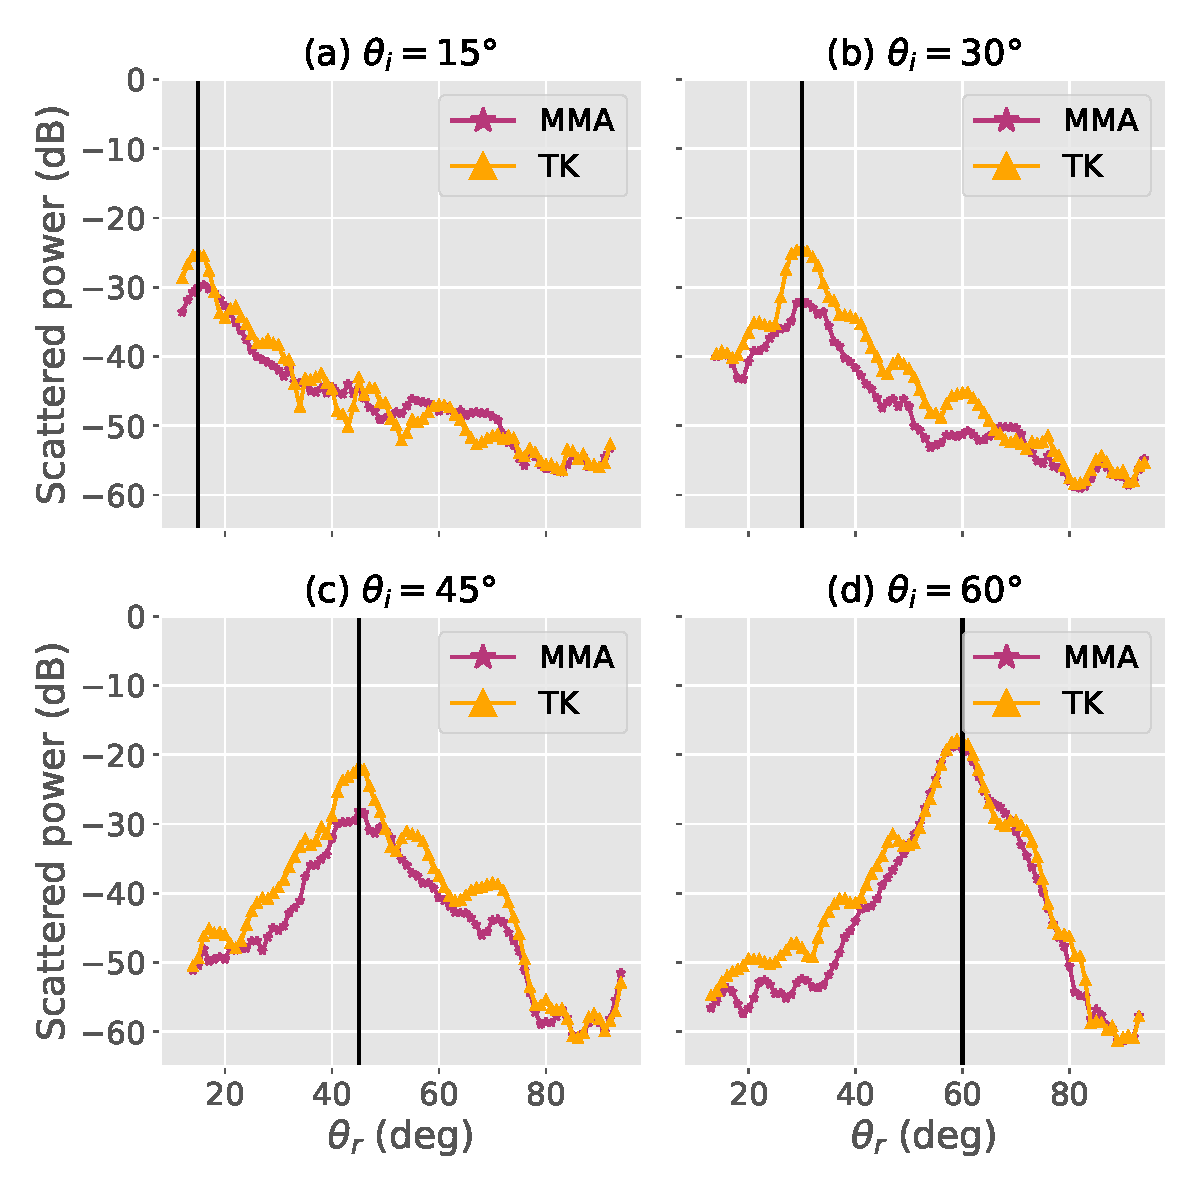
\includegraphics[width = \textwidth]{scatter_3_2020.pdf}
    \caption{Scattering measurement. The four panels show front scattered power off the sample with the source located at four angles of incidence $\theta_i$: (a) \,15$^{\circ}$, (b) \,30$^{\circ}$, (c) \,45$^{\circ}$, and (d) \,65$^{\circ}$. The source was set at 110\,GHz. Each of the measured data points was averaged over 17 different sample rotation angles, from which the associated error bars were also estimated. The error bars are too small to be visible at these y scales. The vertical black lines indicate the position of the specular reflection directions. The blue data points show the results from the MMA tiles, while the red data points show the results from the TK tiles. The TK tiles are measured to have an overall higher scattering than the MMA tiles, which leads to a higher integrated scattering power, as shown in Table~\ref{tab:scat}.}
    \label{fig:scatter}
\end{figure}

\begin{table}[ht]
\centering
\begin{tabularx}{0.45\textwidth}{>{\centering\arraybackslash}X >{\centering\arraybackslash}X >{\centering\arraybackslash}X}
    \hline
    \hline
    $\theta_\text{I}$ & $15^{\circ}$ & $30^{\circ}$ \\
    \hline
    MMA & $0.49\pm0.03$\% &$0.12\pm0.002$\% \\
    TK  & $0.67\pm0.02$\% &$0.53\pm0.01$\%  \\
    \hline
    \hline
    $\theta_\text{I}$ & $45^{\circ}$ & $60^{\circ}$ \\
    \hline    
    MMA & $0.27\pm0.01$\% &$1.98\pm0.02$\% \\
    TK  & $0.83\pm0.01$\% &$2.24\pm0.02$\% \\
    \hline
\end{tabularx}
\caption{Integrated scattering power (in percentage) with different source angle of incidence $\theta_\text{I}$ at 110\,GHz for MMA and TK tiles. Integration is from $\theta_\text{R}=$ $0^{\circ}$ to $45^{\circ}$ away from the specular reflection direction. The cited error is calculated from the standard error of the mean over the 17 repeated measurements for each angle of incidence.}
  \label{tab:scat}
\end{table}

The integrated scattering power is calculated by integrating the scattering over the corresponding solid angles (Eq.~\ref{eq:scat}). The sample's fractional integrated scattering power, denoted as \textit{S}, is normalized by the total integrated input power where \textit{B} is the sample measurement, \textit{A} is the normalized aluminum plate reflection and scattering profile, and $\theta_r$ is receiver angle.

\begin{equation}
\text{S} =\int_{0}^{\frac{\pi}{4}} \text{B} \sin(\theta_\text{r}) d\theta_\text{r} \bigg/ \int_{0}^{\frac{\pi}{4}} \text{A} \sin(\theta_\text{r}) d\theta_\text{r}.
\label{eq:scat}
\end{equation}

This work does not include the power beyond 45\dg{} ($\pi/4$) away from the specular reflection direction, considering its negligible contribution. I calculate the integrated scattering power for our MMA tiles and the TK tiles, listed in Table~\ref{tab:scat}. The results demonstrate the MMA tiles have lower integrated scattering power compared to the TK tiles, meeting the 1\% requirement for angle of incidence $\leq 45^{\circ}$.

\section{Future Applications}
\label{sec:future_applications}
Flat and square MMA tiles were manufactured, in quantities of $> 10,000$, for more general use. The square tiles come in the size of 2.5\,cm $\times$ 2.5\,cm with the same anti-reflection coating (Fig.~\ref{fig:square_tiles}). Each of the flat tiles weigh $\sim$\,4\,g. Tessellating features cover the sides of the square tiles: two sides of the square overhang as lips, while the other two sides indent. These features enable seamlessly tessellating copious number of tiles together. Given the limited thickness ($\sim$\,6\,mm), an injected nut cannot be installed; instead a shaft was designed on the back for alignment. For fastening, four over-sized M2 screw holes were designed on the tessellating lip. Correspondingly, four recesses for the screw head (from adjacent tiles) were designed on the tessellating dent (see Fig.~\ref{fig:square_tiles}). This version of MMA tile is designed to be applied on any flat surfaces by tessellation. They are already used to cover both sides of the Lyot stop in the SO LATR optics tubes (as shown in Fig.~\ref{fig:latr_ot}). The tile-covered Lyot stop assembly has been tested at 4\,K for thermal properties. 



Given the vast potential in customization, the MMA tiles provides a viable solution to blacken cryogenic surfaces with diverse geometries. Therefore, the technology can be useful for many future cryogenic experiments.

\begin{figure}[t]
    \centering
    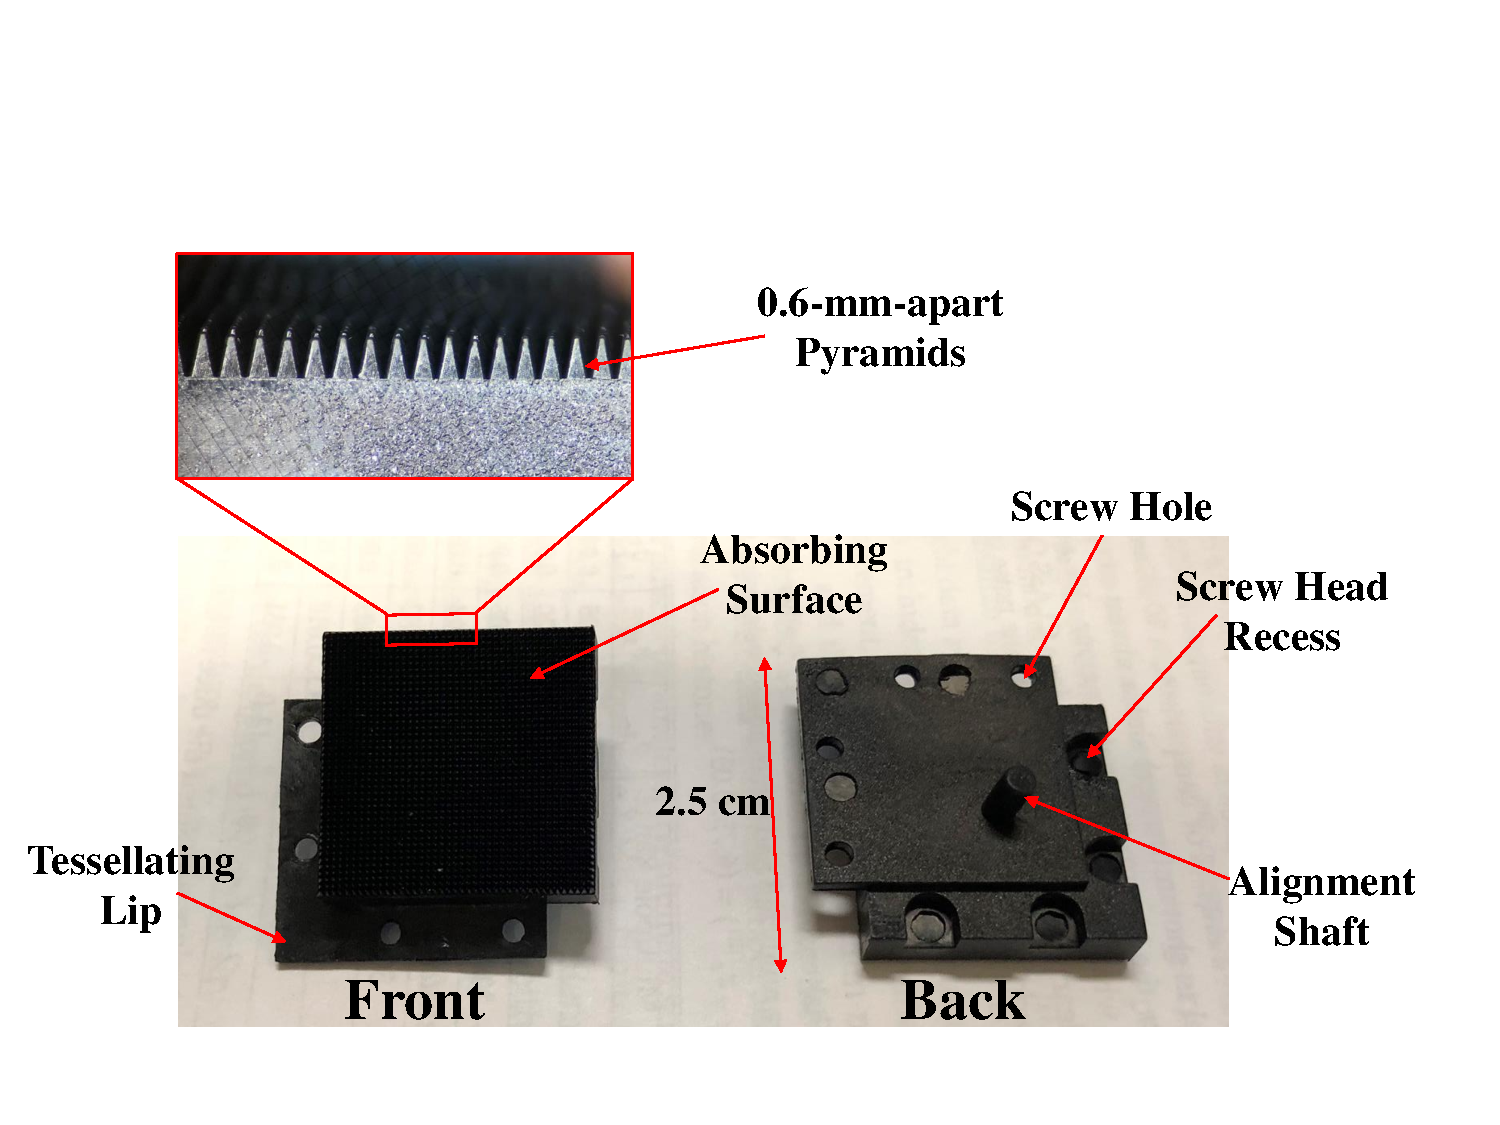
\includegraphics[width=\textwidth]{Figures/square_tiles.pdf}
    \caption{Manufactured square tiles. The 2.5\,cm $\times$ 2.5\,cm flat tiles are also manufactured via injection molding with the same pyramidal structure on the absorbing surface. The main photo on the bottom shows two square tiles from the front and the back. Major features on the tiles were denoted as well. A microscope photo of the pyramids is shown on the top left. The photo shows sharp features of the pyramids, which are only 0.6-mm wide and 1.5-mm tall. The pyramids show sharper features compared to the ones in the tilted tiles (Fig.~\ref{fig:real_tile}). That is because the square tiles are smaller with a simpler shape, which facilitates the manufacturing process.}
    \label{fig:square_tiles}
\end{figure}

\section{Discussion}
\label{sec:conclusion}

The metamaterial absorber (MMA) provides an effective, novel, and low-cost solution to absorb millimeter-wave radiation at cryogenic temperatures. Once the injection mold is manufactured, the tiles are mass-produced at low cost ($<$ 1/10 of conventional methods) with a thousands-per-month production rate. Both the initial mold machining and injection molding were performed completely by an external shop, without any involvement from the research group. In addition, the technology also enables a high level of customization in the design. For future cryostat development, customized tiles can be designed and manufactured in this way to achieve the enhanced absorption properties, while fitting the geometry of specific cryostat designs.



The absorber was successfully cooled down to 1\,K with a single thermal contact. The optical properties, including specular reflection and scattering, were measured at different angles of incidence in the frequency band from 90\,GHz to 170\,GHz. The specular reflection is $< -30$\,dB for angles of incidence $\leq45$\dg{}. Even at 65\,\dg{}, the specular reflection is only $\sim-15$\,dB. The integrated scattering power is less than 1\% with the angle of incidence $\leq45$\dg{}. Even though this application was tailored for the frequency band from 90\,GHz to 270\,GHz, the metamaterial anti-reflection coating parameters can be suitably adjusted for use at longer wavelengths. The carbon grain size of this commercially available material and the injection molding process limit the suitability of direct scaling this design to shorter wavelengths. The use of a similar dielectric mixture with carbon lamp black and a lower volume filing fraction could be employed to address this challenge.

The design philosophy breaks the overall surface into basic tiles, facilitating their application to an extended surface. Unlike painted absorbing surfaces, the modularized design allows for the easy replacement of tiles, should part of the surface be damaged. The wedge-shape tile introduced in this paper is designed to work in a specific cylinder for Simons Observatory and CCAT-Prime. But different geometries, such as flat square tiles, are also available with similar optical performance.

\chapter{Reflectometry Measurements of the Loss Tangent in Silicon at Millimeter Wavelengths}
\label{ch:si}
The following was published in the proceedings from the 8th ESA Workshop on Millimetre-Wave Technology and Applications in 2018~\cite{ches18}.
\section{Introduction}
Dielectric loss and its associated thermal emission is a key driver for sensitivity in millimeter wave receivers. A low loss implies low emission from a material, therefore limiting thermal noise propagating through to the detector. The
contribution to the thermal noise due to loss,  $T_{\text{sys}}$, can be calculated as:
\begin{equation}
    T_{\text{sys}}=T_{\text{comp}}(L-1)
\end{equation}
where $T_{\text{comp}}$ is the physical temperature of the component, $L=\exp(2\pi n \tan(\delta)/\lambda_0)$ is the optical loss, $n$ is the index of refraction, $\tan(\delta)$ is the loss tangent, $t$ is the sample thickness, and $\lambda_0$ is the free-space wavelength. The noise due to loss can be reduced in two ways: lowering the temperature of the component, and using materials with lower intrinsic loss. 

Many millimeter wave experiments use cold optical components to minimize noise contributions due to this thermal emission. However, in many cases, it is advantageous to include warm silicon components in optical designs. For example, in the ALMA Band 1 receivers include a warm lens that also acts as the window into the cryostat. The original design uses a plastic (high density polyethylene) lens that contributes one-third of the overall receiver noise budget. Substitution of a lens with lower dielectric losses could therefore make a substantial impact on the sensitivity of this instrument.

Silicon is a potentially attractive material for such applications. Datta et al. 2013 showed that silicon can be machined to produce very high quality anti-reflective (AR) meta-surfaces to reduce the reflected power from the natural 30\% to levels in the few tenths of a percent range~\cite{Datta:13}. The key development required is identification of a source of silicon with low dielectric losses at room temperature.

Since it was first reported in Parshin et al.~\cite{parshin} and included in the Lamb 1996 compendium of mm-wave material properties~\cite{lamb}, the promise of silicon as an intrinsically low-loss mm/sub-mm optical material has tantalized the astronomical community.   More recently, Krupka et al. 2016~\cite{KRUPKA201676} reported on the result of a loss tangent in Ka-band and Q-band ($\approx27-40$\,GHz) on the order of $\tan(\delta)\lesssim 10^{-5}$ at room temperature ($\approx300\,K$) for samples of proton-irradiated high purity FZ silicon, but measurements in W-band ($\approx$90\,GHz) and for neutron-irradiated samples are lacking. We address this here using coherent reflectometry measurements.

In Section~\ref{sec:si_procedure} we detail the optical hardware and the receiver electronics used to measure the optical properties.  We also describe the two silicon samples analyzed in this work; intrinsic and neutron-doped silicon.  Section~\ref{subsec:mcmc} details the mathematical model and fitting method used to determine the optical properties from reflectivity data.  The resulting optical properties are presented in Section~\ref{sec:si_results}.  Lastly, we discuss implications of the results for optical performance of the telescope in Section~\ref{sec:si_conclusion}.
\section{Procedure}
\label{sec:si_procedure}
\subsection{Optical Hardware}
A feedhorn source sends a millimeter wave signal to a parabolic mirror, which sends a plane wave toward the sample, typically at a 10$^{\circ}$ angle of incidence. For these measurements, the sample is a dielectric slab immersed in air. A portion of the signal is reflected to the first air-dielectric boundary, and the remaining signal propagates through the sample, where it again partially reflects from the second dielectric-air boundary, leading to a Fabry-Perot interference in the dielectric cavity defined by the sample. The reflected signal propagates to a second mirror, followed by the receiver feed horn. The geometry is shown in Figure~\ref{fig:optical_setup}.

Eccosorb is placed on surfaces outside the beam in order to reduce and absorb unwanted reflections.   The alignment of the receiver is controlled with a three-axis stage. The tilt of the sample is controlled with a three-point micrometer mount.   This angle is chosen by placing an aluminum plate in the sample holder and maximizing the received signal at a single frequency. Once the setup is aligned, a calibration data set is taken by measuring the reflectance of the aluminum plate as a function of frequency. This dataset serves to define perfect reflection.   The aluminum plate is then replaced with the sample (silicon here) and the measurement is made. The response of the silicon sample measurement is divided by the response of the aluminum plate to yield a measurement of the reflectance of the sample as a function of frequency.

\subsection{Receiver Electronics}
A correlation receiver designed for a holography system is used for these measurements. The receiver compares a reference signal to a signal which has passed through the device, creating an interference pattern between the two.   The holographic imaging setup is summarized in Figure~\ref{fig:holog_ref_setup}.   The Re-configurable Open Architecture Computing Hardware (ROACH2) board correlates the reference and modulated signals~\cite{roach2}.

\subsection{Samples: Neutron-irradiated and Intrinsic Silicon}
Two samples were provided by Topsil for testing. The samples as cut exhibited curvature and uneven thickness of approximately 15\,mm. A professional third party was contracted to grind and polish the samples flat and parallel. The
resulting thicknesses are reported in Table 1, and are accurate to scales $\ll \lambda_0$ measured with a micrometer. The silicon is made with Float Zone mono growth in an oxygen-free environment, reducing risk of generating thermal donors during
high temperature processes~\cite{topsil}.
\section{Reflectometry and Transmissivity}
We measured the transmission and reflection of these samples. The data are shown in Figure~\ref{fig:si_data}.
\begin{figure}[t]
    \centering
    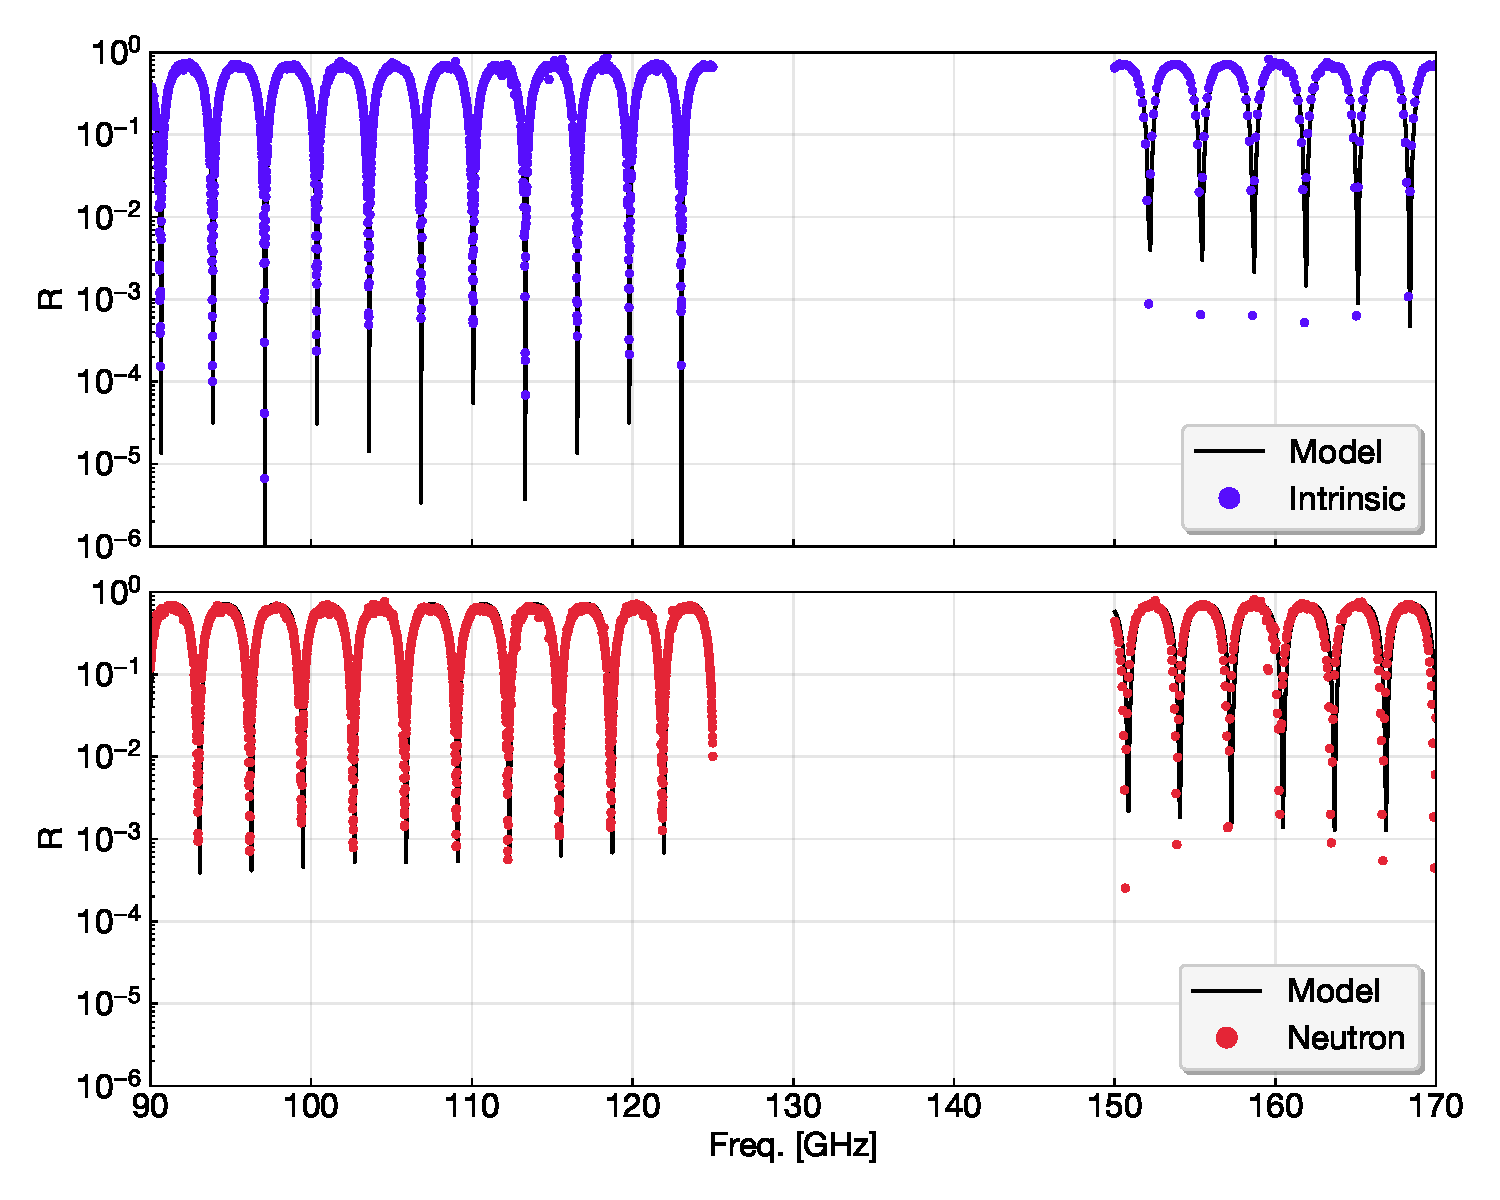
\includegraphics[width = \textwidth]{Figures/silicon_refl.pdf}
    \caption{Reflectivity of intrinsic (top) and neutron-irradiated (bottom) silicon against frequency [GHz].}
    \label{fig:si_data}
\end{figure}
\subsection{Modeling}
\label{subsec:mcmc}
We model the dielectric slab with a complex index $n_2 = n_r + in_i$.  Air is treated with a purely real index $n_1 = $. The refracted angle in each layer is calculated using Snell's law, where $\theta_1$ is the incident angle and $n_1$ is the free-space
index of the first layer (i.e. $n_1$ in Eq.~\ref{eq:snell}). The setup began at an incidence angle of $10^{\circ}$.

\begin{equation}
    \theta_2 = \arcsin\bigg(\frac{n_1}{n_2}\sin\theta_1\bigg)
    \label{eq:snell}
\end{equation}
The experiment exclusively uses TM mode signals, where the reflected and transmitted coefficients theoretically
predicted by~\cite{jackson}:

\begin{equation}
    R = \frac{n_1 \cos\theta_2 - n_2\cos\theta_1}{n_1\cos\theta_2 + n_2\cos\theta_1}
    \label{eq:R_snell}
\end{equation}

\begin{equation}
    T = \frac{2 n_1 \cos\theta_1}{n_2\cos\theta_1 + n_1\cos\theta_2}
    \label{eq:T_snell}
\end{equation}

\begin{equation}
    \tan(\delta) = 2n_i/n_r
    \label{eq:loss}
\end{equation}

Using Eq.~\ref{eq:R_snell} and Eq.~\ref{eq:T_snell}, where the parameter $n_2$ is the fitting parameter, the material index is extracted from measurements. 

\subsection{Fitting}
The loss tangent (or equivalently complex part of the index) leads to a reduction in the depth of the reflection nulls for this signal. The cancellation of the incident and reflected waves is more perfect for lower loss tangent. Therefore, the nulls in the reflection are crucial to get a reliable constraint on the loss. We also note that one of the dominant systematic effects is standing waves between the source and receiver horn. This systematic includes a reflection from the sample. Therefore, this noise is minimized near the nulls. For this reason, we fit the data only where the reflectance is below some threshold (typically $R<0.01$, though, varying this by a factor of a few has no impact on the results). The weighing of each data point scales as the inverse of reflectivity to force the fit to focus on the depth of the nulls. We test that the analysis doesn’t depend on this weighting by doing describe. We implemented a Markov Chain Monte Carlo (MCMC) algorithm for fitting the reflectivity model to our measurements using the Python package \verb|pyMC|, with the real and imaginary components of the index of refraction as fitting parameters~\cite{Patil2010PyMCBS}. The MCMC algorithm samples the probability distribution of each parameter, in this case the probability of two parameters in the reflectivity model matching the measured reflectivity of the sample. This method was used to fit the measurement to the model, yielding, the real and imaginary components of index of refraction of the sample. The loss, $\tan(\delta)$, of the material is then calculated using Eq.~\ref{eq:loss}.

The error bars of loss values are calculated with two methods. The first method is the MCMC error computation with the \verb|pyMC| package in Python. To check these values, each null is fit individually using the MCMC algorithm, yielding an array of parameter values. The root-mean-square (RMS) of these values is then calculated, yielding the RMS error. Both methods yielded nearly equivalent loss error results, and we therefore report the MCMC loss error in Table~\ref{tab:silicon}. The error in index of refraction is not reported as it is likely included in the uncertainty of the thickness, while the MCMC reported a negligible error for this parameter.

\begin{table}
    \centering
\begin{tabular}{ |p{3cm}|p{3cm}|p{3cm}| }
 \hline
 Silicon & Neutron & Intrinsic\\
 \hline
  $n$ & 3.415 & 3.412 \\
 \hline
 $\tan(\delta)\times 10^{-5}$ & $28.93 \pm 1.21$ & $1.47 \pm 0.09$\\
 \hline
  D\,[mm] & $13.68 \pm 0.1 $ & $13.56 \pm 0.1$\\
 \hline
\end{tabular}
    \caption{Optical properties of silicon. Properties extracted from the data when fit with the theoretical model. Properties $n$ is the index of refraction, D is the thickness of the sample, and $\tan(\delta)$ is the loss tangent.}
    \label{tab:silicon}
\end{table}

\section{Results}
\label{sec:si_results}
The index of refraction of neutron and intrinsic silicon are nearly identical, with $n =3.415$ for neutron-irradiated silicon, and $n =3.412$ for the intrinsic silicon samples. The neutron-irradiated sample has $\tan(\delta) = 2.8\times10^{-4}$, while the intrinsic silicon is nearly an order of magnitude better, with $\tan(\delta)= 1.5 \times 10^{-5}$. See Table~\ref{tab:silicon} for a summary of the measured and inferred properties.

The reason for the higher loss in the neutron-irradiated sample is unclear, as the loss tangent should improve for materials with higher resistivity if dominated by the conduction loss term. As the resistivities of the neutron-irradiated and unmodified intrinsic silicon samples were measured by Topsil to be $>100\,k\Omega-cm$ and $>50k\,\Omega-cm$, respectively, the expectation is that the neutron-irradiated sample should have less loss. One possible explanation is that the lattice defects introduced by neutron irradiation contribute to the loss.

\section{Conclusion}
\label{sec:si_conclusion}
We have presented the characterization of optical properties for two silicon samples using a radio holography setup.  The resulting values for the loss $\tan(\delta)$ from MCMC fits to our measurements of the unmodified intrinsic silicon sample are comparable to those reported in Parshin et al. 1995~\cite{parshin}.  Further, our measured low loss in intrinsic silicon demonstrates it can be a compelling material for use in warm optics.  Krupka et al.~\cite{KRUPKA201676} also report a $\tan(\delta) \approx 1.2\times10^{-5}$ for proton-irradiated silicon, which is lower by more than $3\sigma$ than our measurements of intrinsic silicon, but on the same order of magnitude.  Our work shows promise for the use of intrinsic silicon for room-temperature optical components, such as those required for the lower bands of the Atacama Large Millimeter/Sub-millimeter Array (ALMA) and potential future CMB experiments.



\chapter{The Simons Observatory: Characterizing the Large Aperture Telescope Receiver with Radio Holography}
\label{ch:ot_holo}
\section{Introduction}

Simons Observatory (SO) will observe the cosmic microwave background (CMB) temperature and polarization signals using multiple millimeter-wave telescopes~\cite{gali18, so19}.  One Large Aperture Telescope (LAT)~\cite{Niemack:16, Gudmundsson:21,Parshley_2018} and three Small Aperture Telescopes (SAT)~\cite{ali20} together will measure the CMB anisotropies.  SO will provide new constraints on inflationary signals, neutrino mass, and particles beyond the standard model while further improving our understanding of dark energy and galaxy evolution and the era of cosmic reionization~\citep{so19}. 

The LAT is a crossed-Dragone telescope~\cite{6773968,Niemack:16,2021RNAAS...5..100X} developed in collaboration with the Fred Young Sub-millimeter Telescope (FYST)~\cite{ccat,aravena2019ccatprime} Collaboration.  The LAT Receiver (LATR) can hold up to 13 optics tubes, which can accommodate more than 60,000 detectors distributed across 39 detector wafers for CMB studies~\cite{Parshley_2018,zhu2021simons,mccarrick2021simons}.  Each optics tube holds a set of lenses, filters, and baffles which couple light from the telescope onto a set of three polarization sensitive detector arrays.   Realizing the SO science goals depends on achieving stringent sensitivity requirements and controlling systematic effects to be subdominant to the statistical noise.   To achieve this, the optics tubes must have clean beams with well-controlled side-lobe power.  

Testing these aspects of the optics tube performance in the lab is challenging.  Previously, these parameters were verified on ground-based CMB radio telescope systems upon deployment~\cite{alma_holog,2007A&A...465..679N}.  In this paper, we present a new approach to laboratory testing of these systems using the technique of near-field radio holography.  Holography is an instrumentation technique used to measure the complex monochromatic electric field wavefront using the interference between a modulated and non-modulated signal.  Radio holography takes advantage of the antenna theory relationship: the far-field radiation pattern of a reflector antenna is the Fourier Transformation of the field distribution in the aperture plane of the antenna~\cite{alma_holog}.

\begin{figure}[ht]
    \centering
    \includegraphics[width = .8\textwidth]{Figures/lat15.pdf}
    \caption{The Simons Observatory (SO) Large Aperture Telescope (LAT), featuring a segmented primary and secondary mirror.  The mirror's focus is hidden inside the conical baffle near the front of the receiver.  The receiver can hold up to thirteen optics tubes.}
    \label{fig:lat}
\end{figure}

Within radio beam characterization, several techniques exist; 1) scalar beam pattern characterization~\cite{doi:10.1063/1.3292308}, or measuring only the magnitude of the wavefront, 2) vector beam pattern characterization~\cite{2020JLTP..199..156Y,7740846}, or measuring the amplitude and phase of the wavefront, and 3) holographic beam pattern measurement~\cite{387181,7740846}, which we explore here.  While scalar beam pattern characterization requires the beam to be measured at multiple planes along the propagation axis, and vector beam characterization records one complex map, holography records two beam maps (one modulated by the optical element and the other used as a reference) to reconstruct the complex wavefront~\cite{4584681,alma_holog}.

Near-field holography allows us to study the wavefront as it emerges from the optics tube, in the time-reverse sense, from the cryostat.  Using Fresnel diffraction (FD)~\cite{Goodman2005-ne}, these measured fields can be propagated through the optical system to determine the spilled power past the mirrors of the telescope and the far-field beam pattern of the telescope fed by this receiver.  Moreover, these beams are useful for the identification and mitigation of optical problems within the receiver (i.e. optical aberrations, focus, scattered power, etc.).  These measurements enable a detailed verification of system-level optical performance prior to the deployment of a receiver on a telescope.

In Section~\ref{sec:optics_tube} we describe the optical design and components of the SO optics tube.  In Section~\ref{sec:meas_method} we describe the measurement approach including the cryogenic receiver (\ref{sec:meas_method}.\ref{sec:cryo_rec}) and holography hardware (\ref{sec:meas_method}.\ref{sec:meas_hardware}) required for measuring beam maps (full details can be found in Appendix~\ref{app:holog}).  In Section~\ref{sec:results} we present the measured beam maps.   Section~\ref{sec:prop_fields} discusses analysis methods to propagate the measured beams into the far-field using FD.  We present characterization of the optics tube with and without an infrared-blocking filter in Section~\ref{sec:filter}.  Section~\ref{sec:code} details the publicly available code.  We conclude with a discussion of future applications of this approach in Section~\ref{sec:discussion}.  

\section{SO Large Aperture Telescope Optics Tubes Design}
\label{sec:optics_tube}

The LAT is a crossed-Dragone telescope with a 6\,m pupil diameter (Fig.~\ref{fig:lat}).  The LAT Receiver is designed to house thirteen optics tubes, which guide photons onto cryogenic detectors.  These optics tubes must maintain excellent beam quality while also limiting the wide-angle scattering.  The scattering is critical to the ultimate sensitivity of the SO LAT since every percent that is scattered leads to 3\,K of extra noise and a 15(10)\,\% reduction in mapping speed in the 90(150)\,GHz bands which are critical for the SO science.

\begin{figure}
    \centering
    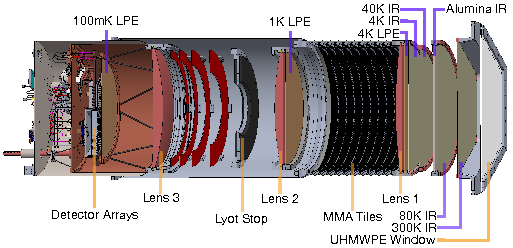
\includegraphics[width = .9\textwidth]{Figures/LATR_OT_Tester_20190221_3.pdf}
    \caption{The Simons Observatory LATR optics tube.  Light enters the optics tube from the right through an ultra-high-molecular-weight polyethylene (UHMWPE) window, and travels through a series of Infrared-Blocking filters (IR), including one alumina IR filter, and passes through the 4\,K Low-Pass Edge mesh filter (LPE). The light is focused on the detector arrays on the left by the three lenses, with two additional LPE filters near the 1\,K and 100\,mK stages.  The components within the optics tube are further described in~\cite{xu/etal:2020c}.}
    \label{fig:latrt}
\end{figure}


Figure~\ref{fig:latrt} shows the LATR optics tube~\cite{xu/etal:2020c}.  Light enters through a 3\,mm thick ultra-high molecular weight polyethylene hexagonal window with an anti-reflection coating~\cite{zhu18}.  Three anti-reflection coated silicon lenses~\cite{Datta:13,golec20} control the beam size and shape, which re-images from the focal plane onto three hexagonal detector wafers.  Each lens is accompanied by a low-pass edge filter (LPE)~\cite{10.1117/12.673162}.  The light is coupled onto the detector wafers using arrays of drilled spline profile feed horns and the polarization is coupled onto the wafer with an orthomode transducer~\cite{10.1117/12.2313405,2022arXiv220104507H}.  Along this path, the light passes through a succession of band-defining and infra-red blocking filters~\cite{10.1117/12.673162}.  From the sky side these are a 300\,K IR blocking filter, an 80\,K IR blocking filter, an 80\,K IR rejecting metamaterial anti-reflection coated alumina filter~\cite{golec20,golec2022}, and a 40\,K IR blocking filter~\cite{10.1117/12.2561720} prior to entering the optics tube.  The filter configuration is described in~\cite{zhu18}.  Between lenses 1 and 2, the walls of the optics tube are coated with baffling metamaterial tiles, described in~\cite{Xu:21}, which control scattering.  The full cold-optical design is described in~\cite{dicker2019cold}.  All optical elements in the optics tube are between 4\,K and 100\,mK.

\section{Measurement Approach}
\label{sec:latot_meas_method}
Here, we describe the hardware and software used in these holography measurements.  Further details can be found in Appendix~\ref{app:holog}.  For this discussion we divide the system into a cryogenic system mounted in the optics tube and a holography system comprised of a source, correlation receiver, and motion system.


\subsection{Cryogenic System}
\label{sec:cryo_rec}
The optics tube is housed in a test cryostat called the LATR tester \cite{Harrington_2020}.  The cryostat holds and cools a single optics tube and provides support for detector readout.  This setup supports up to three detector arrays.   In the test configuration, two are bolometric arrays~\cite{2022arXiv220104507H} and the third is used for the holography measurements. 

The holography array consists of a feedhorn array identical to that used for the bolometric detectors, but with standard wave guide flanges at the outputs. A receiver consisting of a round to rectangular wave guide transition and a harmonic mixer is attached to this feed array.  The mixer was designed to operate from 70-110 GHz, but was found to operate satisfactorily up to 170 GHz. For operational simplicity, we used this mixer over our full frequency range from 80-170\,GHz.% -- though there is some evidence it becomes partially multi-moded towards the upper edge of this range.  
A second identical receiver was also connected for redundancy, but not used in the measurements described here.   Two 0-18\,GHz coaxial connections were made from the receiver to connectors at the cryostat wall.  These coaxes are heat sunk at various stages between the focal plane, which was operated at 4\,K while doing holography, and the 300\,K cryostat wall.  A separate cool down was used to measure the loss along these coaxial feed lines.  The loss  was found to be 23\,dB at the LO frequency (10-13\,GHz).  Accurate knowledge of the loss along the feed lines is critical for providing the correct amount of power to the mixers in the focal plane.  The loss at the interference frequencies (IF) (100\,MHz) is significantly lower and not critical to the function of this system.

\begin{figure}
    \centering
    \includegraphics[width = .95\textwidth]{Figures/LATRt_isometric.pdf}
    \caption{Schematic of holography setup.  Two local oscillators (LO's) supply frequencies ($f_1$ and $f_2 = f_1+f_{\text{offset}}$), one serving as a non-modulated reference signal, while an active multiplier modulates the other.}
    \label{fig:setup}
\end{figure}

\subsection{Holography System}
\label{sec:meas_hardware}

Figure~\ref{fig:setup} shows a schematic overview of the LATR tester (LATRt) holography hardware.  Two millimeter-wave sources are used to measure the full SO MF band: F90 (80-120\,GHz) and F150 (130-170\,GHz).  Only one is mounted at a given time.  These sources are broadcast into the receiver using standard gain feed horns held close to the window (4.5\,cm in F90 and 11.5\,cm in F150 due to the different attenuator waveguide lengths).  We therefore expect different measured beam sizes between the two sets of frequencies, since the beam expands as it leaves the optics tube.
 


A motorized two-dimensional  stage holds the source and is mounted on a support structure above the LATRt.  During a measurement, the source (frequency is fixed) is moved over a $50\times50$\,cm range with 0.25\,cm steps (black arrows in Figure~\ref{fig:setup}).   One map takes roughly 12 hours to complete.

A common local oscillator (LO2 in Figure~\ref{fig:setup}) is fed to two harmonic mixers: 1) picked off from the source and 2) at the output of the cryogenic receiver.  The IF signal from both mixers in the ~0-100\,MHz band is amplified and passed to a digital correlator (Casper ROACH2 ~\cite{roach2}) which computes the complex correlation between the two signals~\cite{ches18}.  The FPGA on the ROACH2 board outputs the amplitude and the phase of the correlated output, subdivided into a number of 100\,kHz wide bins.  Only the bin associated with the IF frequency is used in subsequent analysis.  The software to program and analyze output from the FPGA is made public on the \textit{McMahonCosmologyGroup} GitHub page in a package called \verb|holog-exp|~\cite{holog-exp}.  Appendix~\ref{app:holog} provides further details to the hardware of the holography setup.


\begin{figure*}[ht]
    \centering
    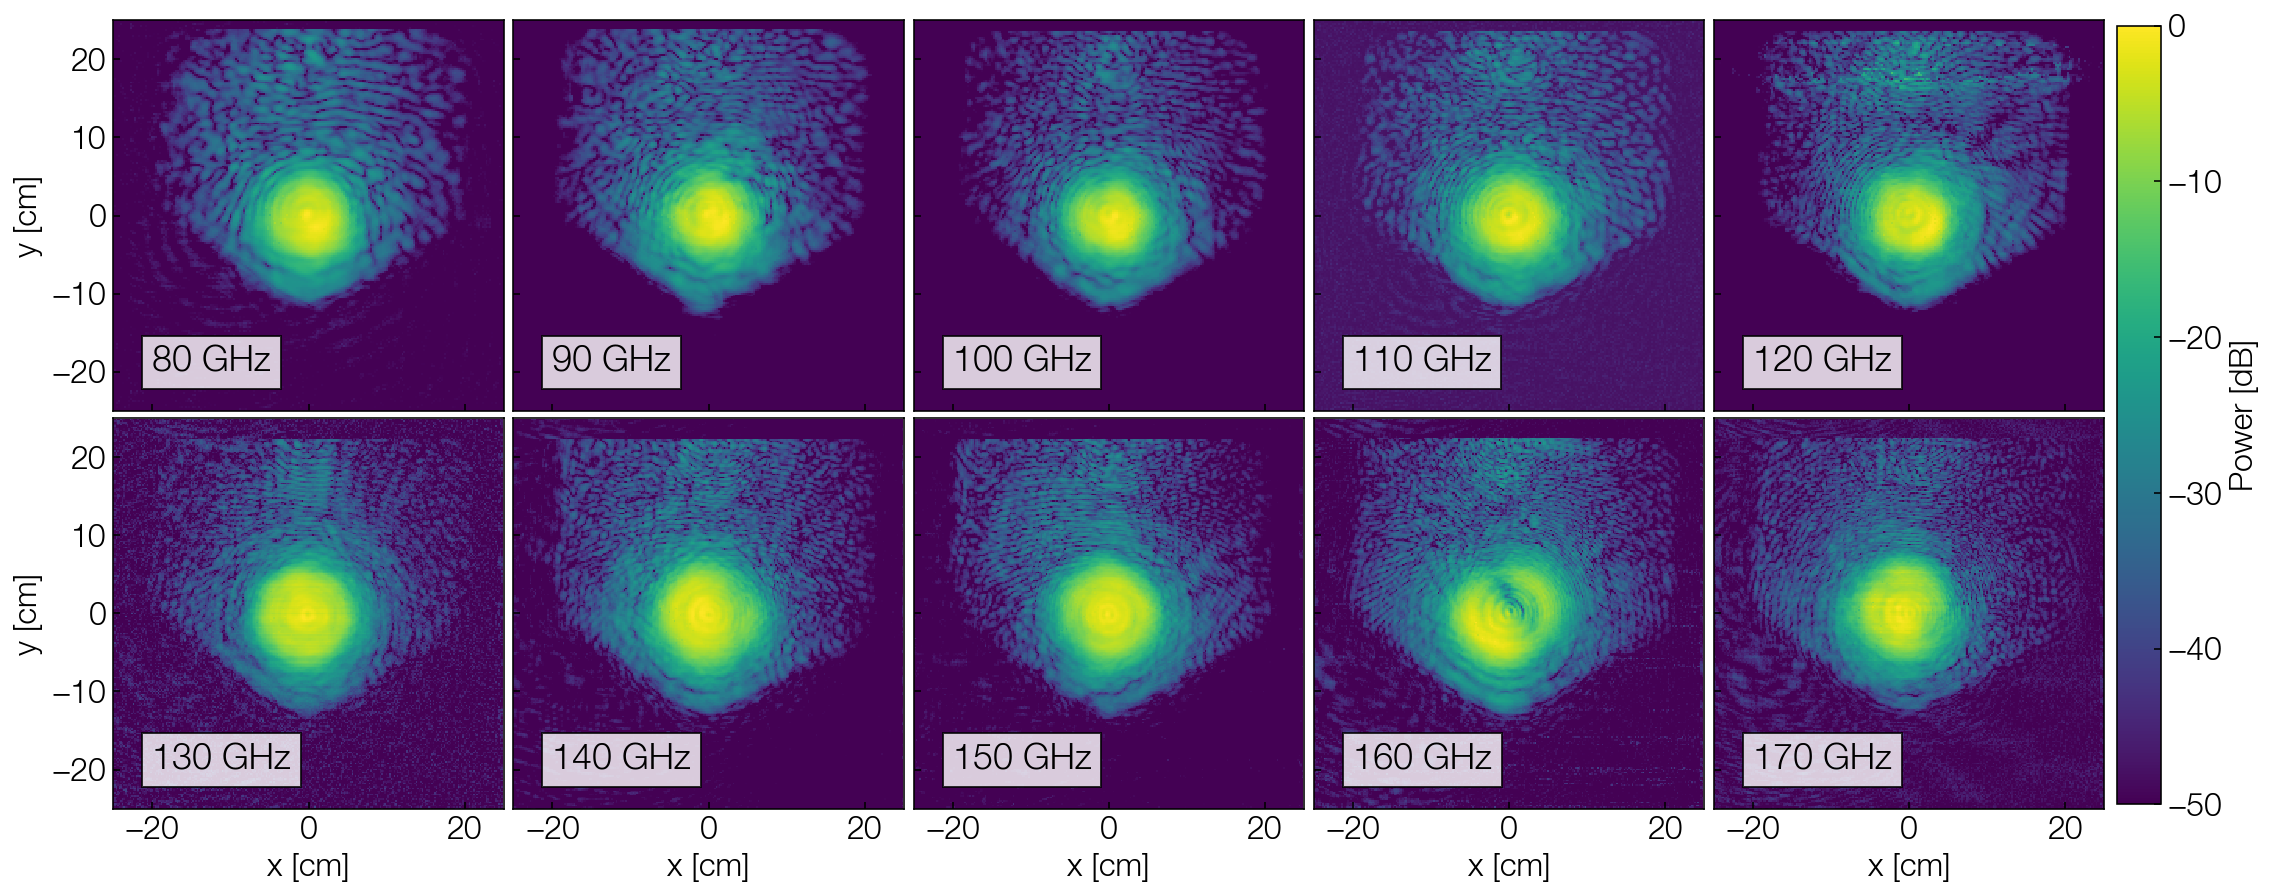
\includegraphics[width = .95\textwidth]{Figures/MF_amp.png}
    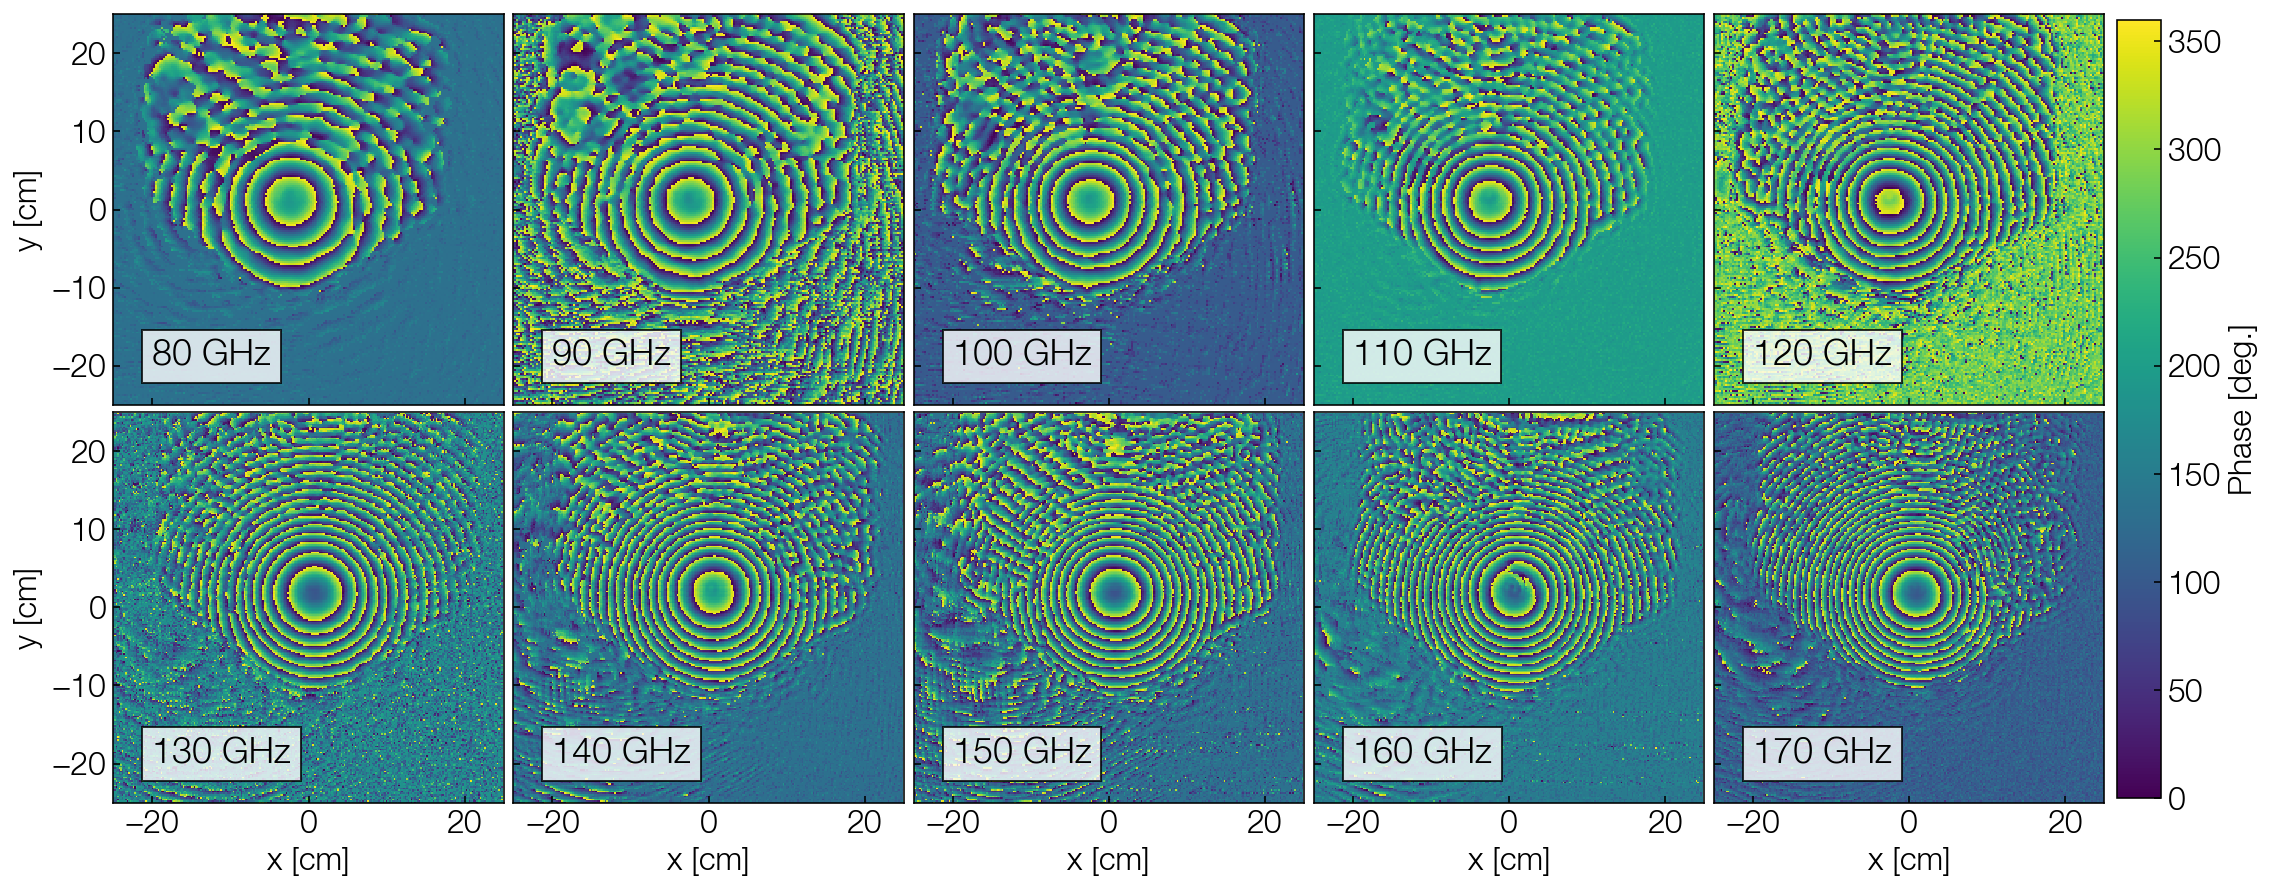
\includegraphics[width = .95\textwidth]{Figures/MF_phi.png}
    \caption{Holography beam map measurements in the mid-frequency band.  Top: Power at each measured frequency (peak-normalized in each map).  Bottom: Wrapped phase at each measured frequency.}

    \label{fig:beam_measurements_all}
\end{figure*}

\section{Results and Interpretation}
\label{sec:results}
\subsection{Near-Field Beam Maps}
Figure~\ref{fig:beam_measurements_all} shows the power and phase of the beam maps at each frequency for which the measurement was carried out.   A variable attenuator at the output of the source was used to optimize the amount of signal entering the optics tube, to ensure power was not too high such that the measurement was saturated, but to also ensure the signal was high enough for signal-to-noise greater than 45\,dB.  As stated in Section ~\ref{sec:meas_method}.\ref{sec:meas_hardware}, the F90 source hangs closer to the window than the F150 source (due to different attenuator lengths), and for this reason, we expect the F90 beams to be smaller than the F150 beams.

The shape of the main beam was found to be in good agreement with simulations at all frequencies.  The asymmetric feature seen in the main beam at 160 GHz is believed to be associated with an extra mode in the round wave-guide of the receiver.  Even with this feature, the radial profile is in very good agreement with the theoretical prediction (within 10\% at the -20dB level).   The hexagonal side-lobe seen in each beam map are associated with scattering from within the optics tube and out the hexagonal window.   The phase indicates the field of these side-lobes is diverging less quickly than that of the main beam.  

\subsection{Propagation of Fields}
\label{sec:prop_fields}

\begin{figure*}[ht]
    \centering
    \includegraphics[width = .98\textwidth]{Figures/ff_secondary.pdf}
    \caption{All beam maps propagated at the secondary illumination of the Large Aperture Telescope.  The spilled power to 300\,K is calculated by integrating power outside the boundary of the secondary (red line) with respect to total integrated power of the map.}
    \label{fig:secondary}
\end{figure*}

The performance of the LAT optical system is assessed in detail by using the amplitude and phase of the measured beams to calculate the fields as they propagate through a virtual telescope.  This enables calculation of the far-field beam of the telescope, and the amount of signal "spilled", or lost, at the LAT secondary mirror.  This represents a unique capability of holography measurements which is critical in assessing the overall performance of this system. 

\subsubsection{Fields at Secondary Illumination}
To determine the amount of power "spilled" to 300\,K, we propagate the measured fields forward and onto the plane of the secondary mirror (approximately 12\,m away from the measurement plane.  This is carried out by using the Fourier relationship between the near-field $E(x,y)$ and far-field $B(\theta_x,\theta_y)$ beams \cite{McIntosh2016,alma_holog}:

\begin{equation}
    B(\theta_x,\theta_y) = \int_{\text{aperture}} E(x,y) e^{ i \frac{2\pi}{\lambda} (\theta_x x + \theta_y y )} dx dy 
\end{equation}
where the complex electric field $E(x,y)$ is integrated over the area of the aperture, and $\lambda$ is the wavelength.

Figure~\ref{fig:secondary} shows beam maps propagated to the secondary mirror of the LAT, with the boundary  of the secondary mirror in red.  To quantify the spilled power, we integrate the power outside the boundary, and then normalize to the total integrated power of the beam map.  We find the average spilled power in the F90(150) detector band is 0.65 (0.68)\% with no significant frequency dependence.  This is below the design target of 1\% and indicates the sensitivity of SO should not be compromised by spilled power to 300\,K. 

\subsubsection{Far-Fields}

To propagate the measured near-fields into the far-field, we use a virtual telescope to produce the fields from a distant (100\,km) point source on the measurement plane.  We then multiply this field with the measured near-field beam in the corresponding plane.  Integrating the resulting field over the area of the focal plane produces the amplitude and phase of the far-field at that point.  We then rotate the telescope in azimuth and elevation and repeat this process to produce a full beam map in the sky.

\begin{figure*}[t]
    \centering
    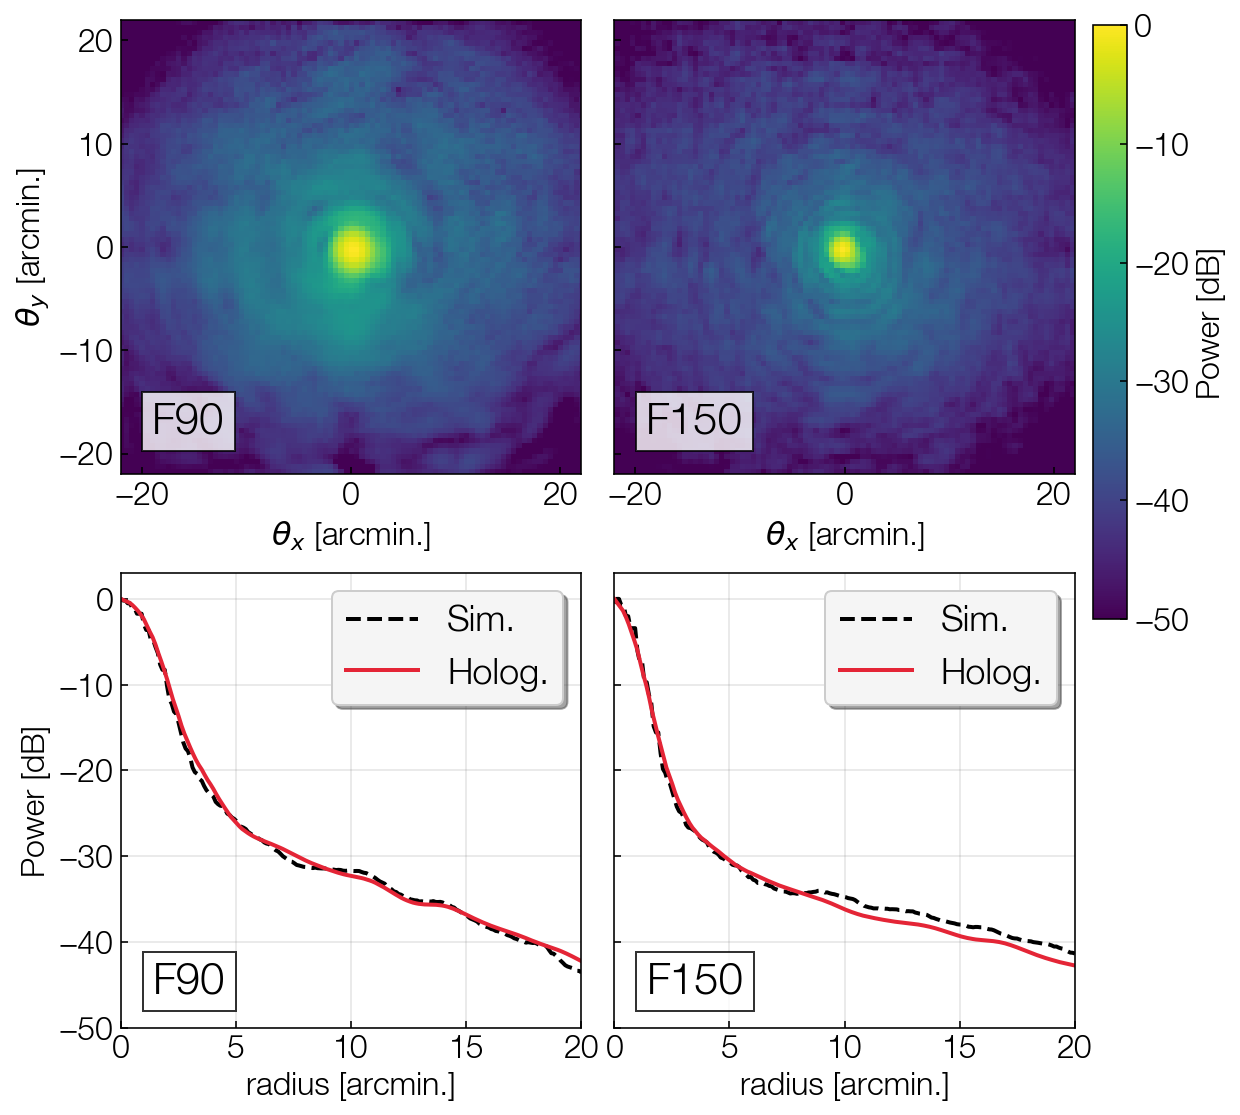
\includegraphics[width = .8\textwidth]{Figures/farfield1d.png}
    \caption{Top row: Using FD, the LATRt measurements are propagated through the LAT from the near-focal plane, to the far-field.  Bottom row: Radial profile of the measured(simulated) far-field beams in the F90 and F150 bands, plotted in red(black).}
    \label{fig:farfields}
\end{figure*}

The holography source emits its signal out of a rectangular feedhorn with a finite size.  The resulting near-field beam is convolved by this rectangular aperture~\cite{2005ifo..book.....G}.  Interpreting this measurement requires accounting for this effect, which amounts to a convolution of the electromagnetic field from the optics tube with the field pattern on the aperture of the feedhorn.  The impact of this convolution is to broaden the F90(150) far-field beam by 12.2(4.7)\% and to create square diffraction spikes in the raw far-field calculation~\cite{2005ifo..book.....G}.

We account for this effect with forward modeling, which is described in Appendix~\ref{app:holog}.  To fully simulate the far-field beam of the LAT including the optics tube, we first simulate the optics tube using \verb|solat-optics| as described in~\cite{holog_sim_model}.  This produces the near-field beam at the front of the optics tube, which is then propagated into the far-field the same way the measured near-field beams are propagated through the virtual telescope.  The resulting far-fields after diffraction spike removal are shown in Figure~\ref{fig:farfields}.  These plots are band averaged, including data from 80-110\,GHz in the F90 band and 130-170\,GHz in the F150 band.  The radial binned far-field holography data are compared to simulations.  These comparisons show that the holography data are consistent with the predicted F90(150) FWHM is 2.18(1.38) arcmin and with low ellipticity with no unexpected features such as the "little-buddies" seen in the ACTPol experiment \cite{2021arXiv211212226L,Gudmundsson:21}.

\section{Filter Removal}
\label{sec:filter}
We have described the holography results from the final instrument configuration.  However, in the initial SO configuration, which contained an additional filter (1K Low-Pass Edge (LPE) filter in Figure~\ref{fig:latrt}), we found extra signal outside the main beam from the window (hexagon at ~-20dB) at all frequencies.  While these side-lobes did not significantly change the spilled power to 300\,K, they would have reduced optical efficiency and led to an enhancement of near side-lobes of the on-sky beam.

To study the frequency dependence of side-lobe power, we computed the integrated fractional power outside the main beam.  We define the main beam radius as $13.5$\,cm, where the beam drops below -20\,dB.   Figure~\ref{fig:filter_info}B shows the integrated fractional power outside the main beam as a function of frequency, and also the measured reflectivity of the 1\,K 6.8\,cm$^{-1}$ LPE filter~\cite{10.1117/12.673162}.

\begin{figure*}[t]
    \centering
    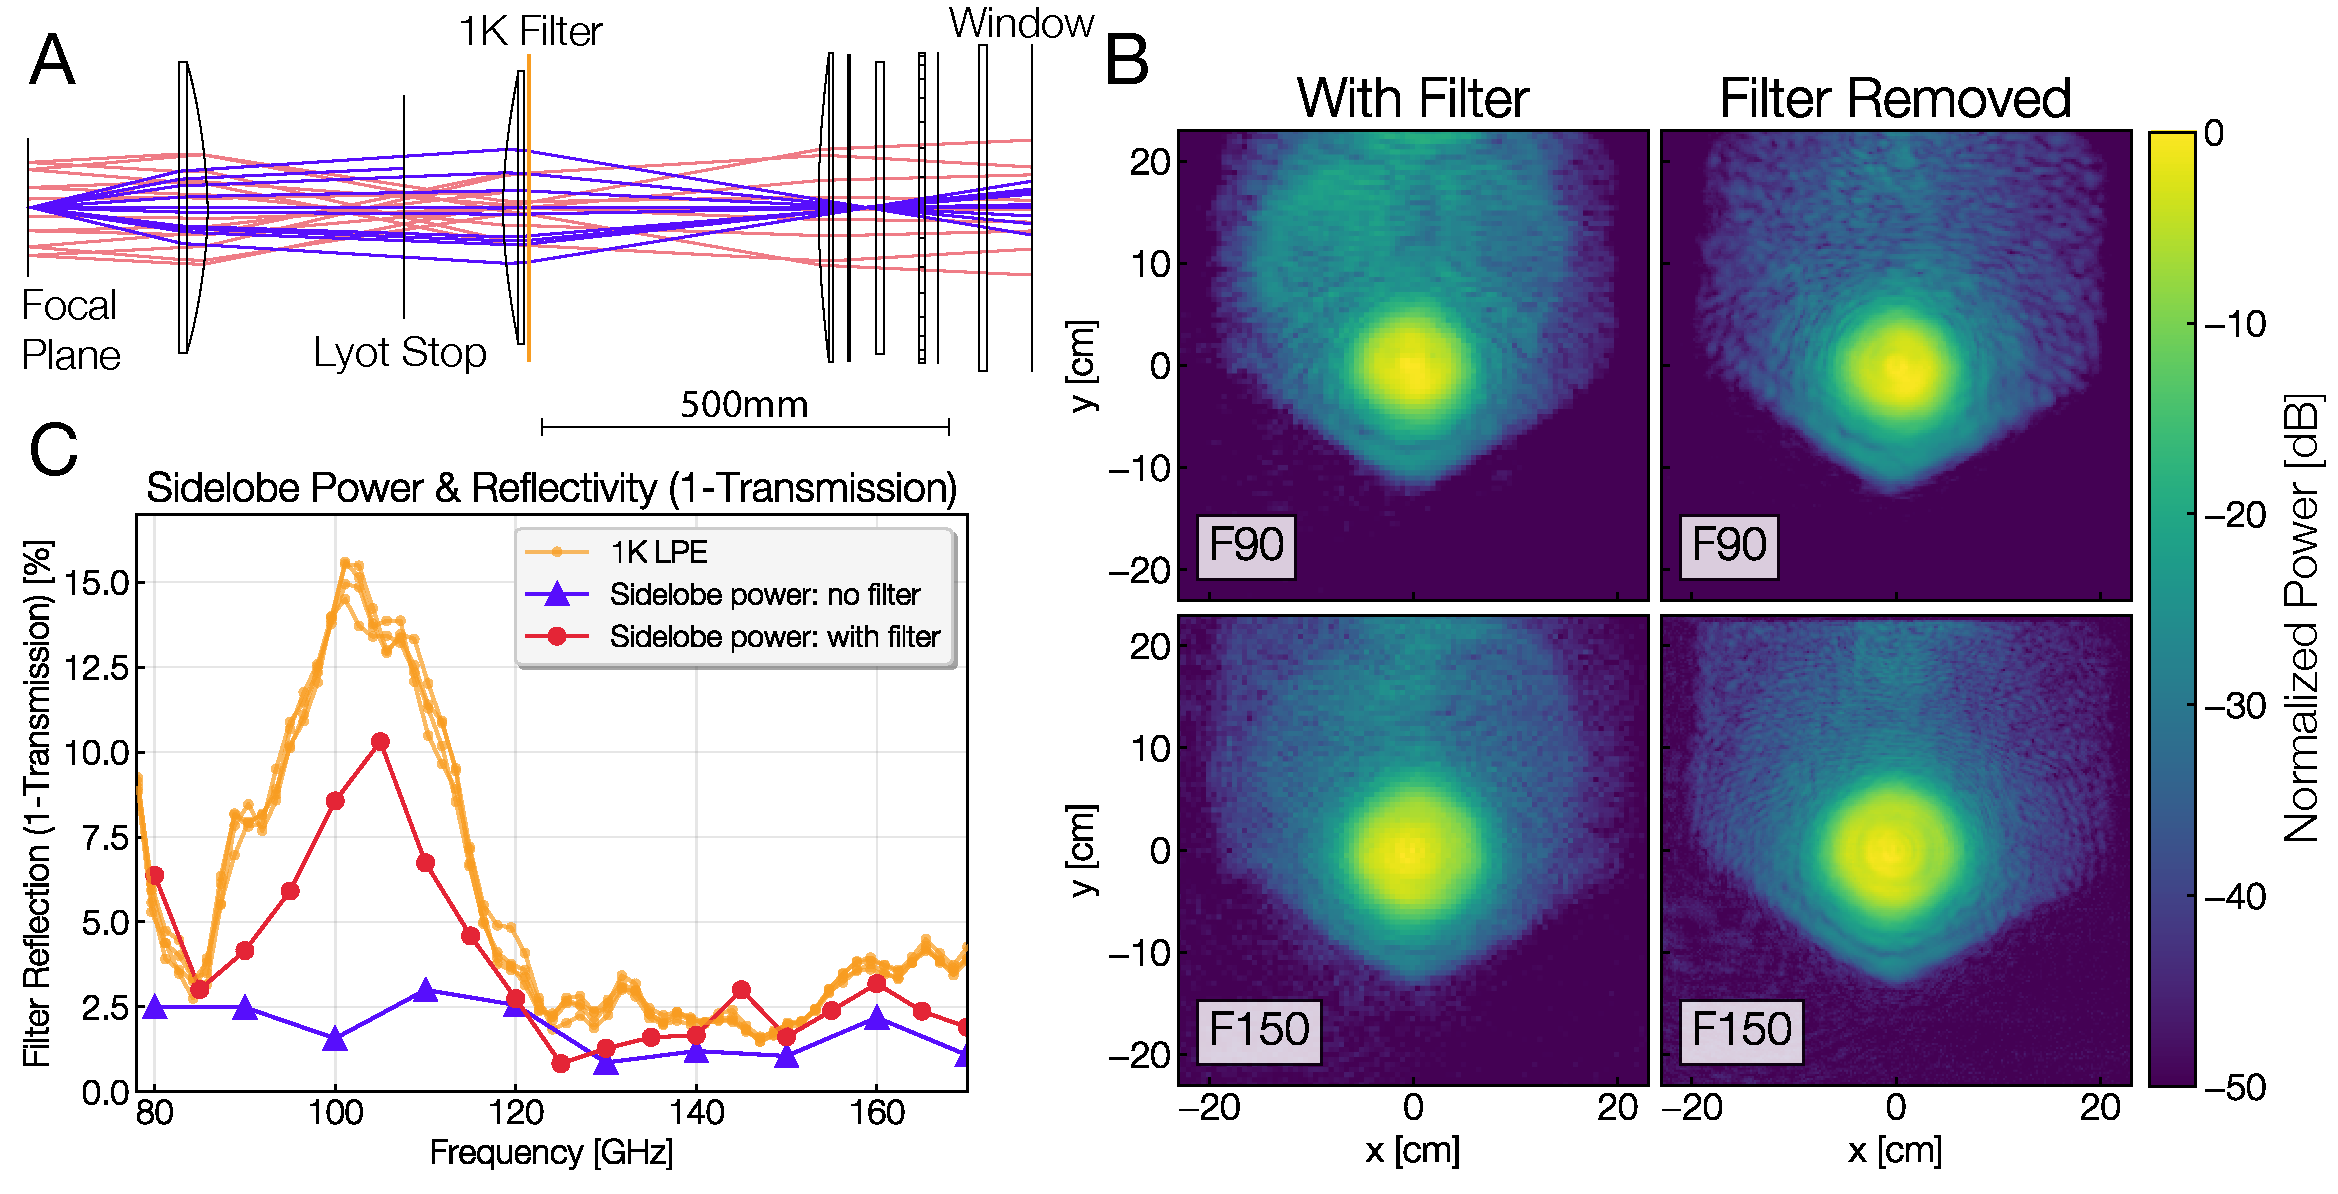
\includegraphics[width = .95\textwidth]{Figures/filter_fig.pdf}
    \caption{A) Time-reversed ray-trace of the SO LAT Optics Tube (OT) with one filter (orange), near the second lens.  With 0\% on-axis reflectivity of the filter, rays(blue) emerge from the focal plane and exit the OT window.  With an on-axis reflectivity of 5.64\,\% (average LPE filter reflectivity in the full band), rays reflected off of the filter(red) go back to the reflective focal plane (copper and reflective), and then propagate out the front of the window.  This is verified in the simulation, as the main beam in front of the OT shows the shape of the focal plane at -25\,dB.  \,\,B) In orange is the measured reflectivity (1-transmission) of the 6.8\,cm$^{-1}$ LPE filter, which is placed at the 1-K stage in the optics tube.  The red(blue) line shows the measured integrated fractional power outside the main beam at each frequency with(without) the filter in the optics tube.  \,\,C) Band-averaged near-field beam maps with and without the filter in the optics tube.  With the filter, beam maps show extra scattering in the top parts of the map, through the upper portion of the LATRt hexagonal window (hexagonal power around the main beam at roughly -20\,dB due to reflection).}
    \label{fig:filter_info}
\end{figure*}

Comparing the side-lobe power to the reflectivity measurements of all filters in the optics tube, we noticed the closest resemblance to the 1\,K LPE filter.  To investigate the effect of a reflective 1\,K LPE filter, a simulation in Zemax~\cite{zeemax} shows the expected measured signal due to reflectivity of a filter (Fig. ~\ref{fig:filter_info}A).  The simulation predicts that rays are reflected off the filter and end up outside the main beam as the rays exit the LATRt window.

After removing the LPE filter from the optics tube and repeating the holography measurements, we measured a decrease in side-lobe power.  Figure~\ref{fig:filter_info}C shows the reduced near-field side-lobe power following the removal of the filter, and the comparison of the side-lobe power with the filter in place.  With the filter removed, the new side-lobe fractional power across the band is 1.9\%, a factor of 3 lower.   The tests presented above do not include this filter.  This provides a concrete example of how holography measurements can be used to optimize cryogenic optical systems.
  
\section{Cross-Polarization}
\label{sec:crosspol}
we measure the polarization performance of the optics tube.  When the source and receiver are aligned, the source emits the TM mode out of the rectangular waveguide, which is measured at the back of the optics tube.  To modulate the polarization of the signal entering the optics tube, we use a polarization grid[CITE GRID ARTICLE].  The grid is made of.... 

We measure the polarized signal for a co- and cross-polarized source.  The co-polar source outputs a TM-mode aligned to the harmonic mixer's waveguide in the focal plane.  We attach a $90^{\circ}$ twist waveguide such that the source's TM output is perpendicular to the harmonic mixer's waveguide.

The model outputs the predicted Stokes parameters received at the back of the optics tube.  Additionally, the receiver is already slightly clocked off of perfect alignment from the source, since the tester-array required slightly tilted holes to mount the receiver.  Therefore, we include this in our polarization model.  We find a degeneracy between the instrument polarization parameters and therefor exclude them in the fit.  We conclude that the holography polarization data is insufficient to quantify the instrument polarization.  

Figure~\ref{fig:holo_crosspol_params} shows the measured power (co- and cross-polarized) as a function of grid tilt, for both co- and cross-polarized sources.  We measure the received power at 85-120\,GHz in 5\,GHz increments, and at grid tilts from 0-360$^{\circ}$, in $10^{\circ}$ increments.  From the data, we use an MCMC to constrain the detector tilt $\theta_{\text{det}}$, grid efficiency $\eta_{\text{grid}}$, and cross polarization $CP$.

Figure~\ref{fig:holo_crosspol_params} shows the constrained parameters obtained by fitting the holography polarization data to the model (Eq.~\ref{eq:holo_model}).  The detector angle $\theta_{\text{det}}$ is constrained to $-30.62^{\circ\,+0.69}_{-0.67}$, the grid efficiency $\eta_{\text{grid}}$ is constrained to $97.00\%^{+0.21}_{-0.22}$, and the cross polarization $CP$ less than $1\%$.  The source emits a polarized signal, which is then additionally polarized by the grid.  For this reason, the holography data cannot constrain the instrument polarization.  We omit the instrument polarization from the model when fitting the holography polarization data. 

\begin{figure*}
    \centering
    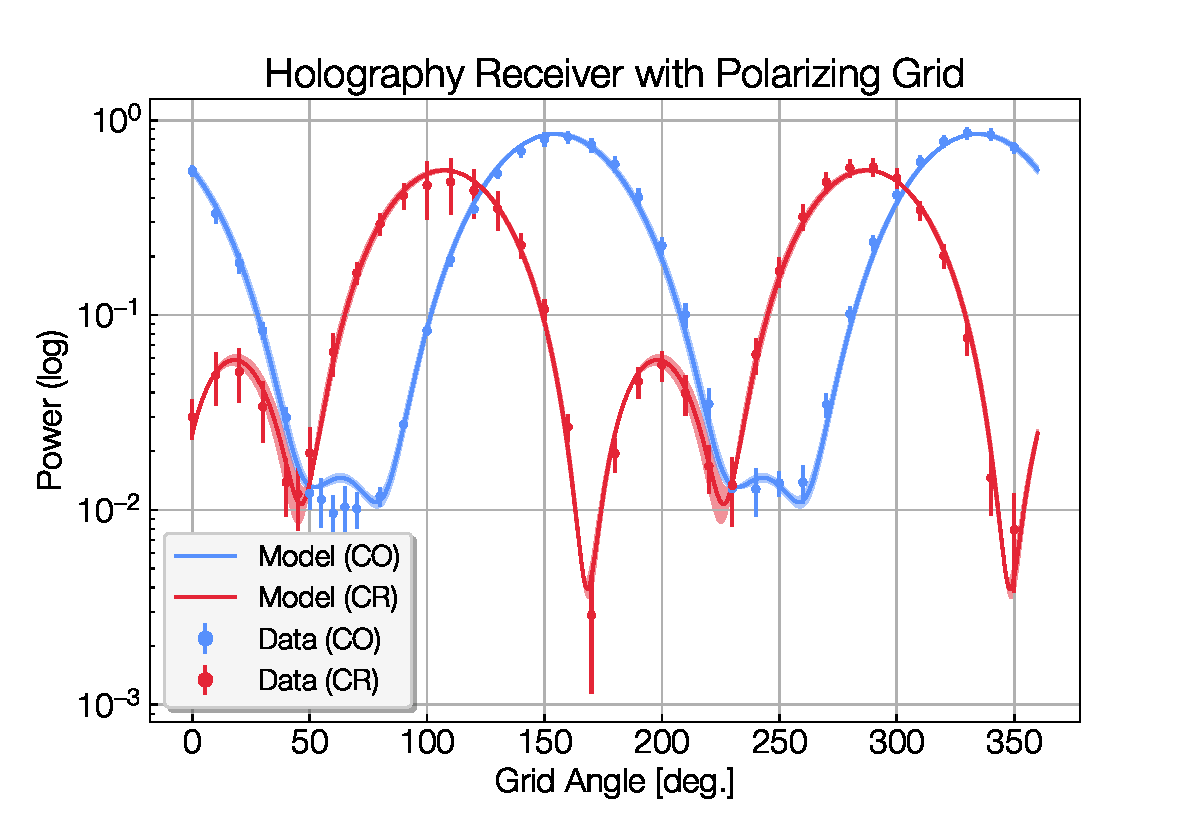
\includegraphics[height = .4\textwidth]{Figures/holo_pol_data.pdf}
    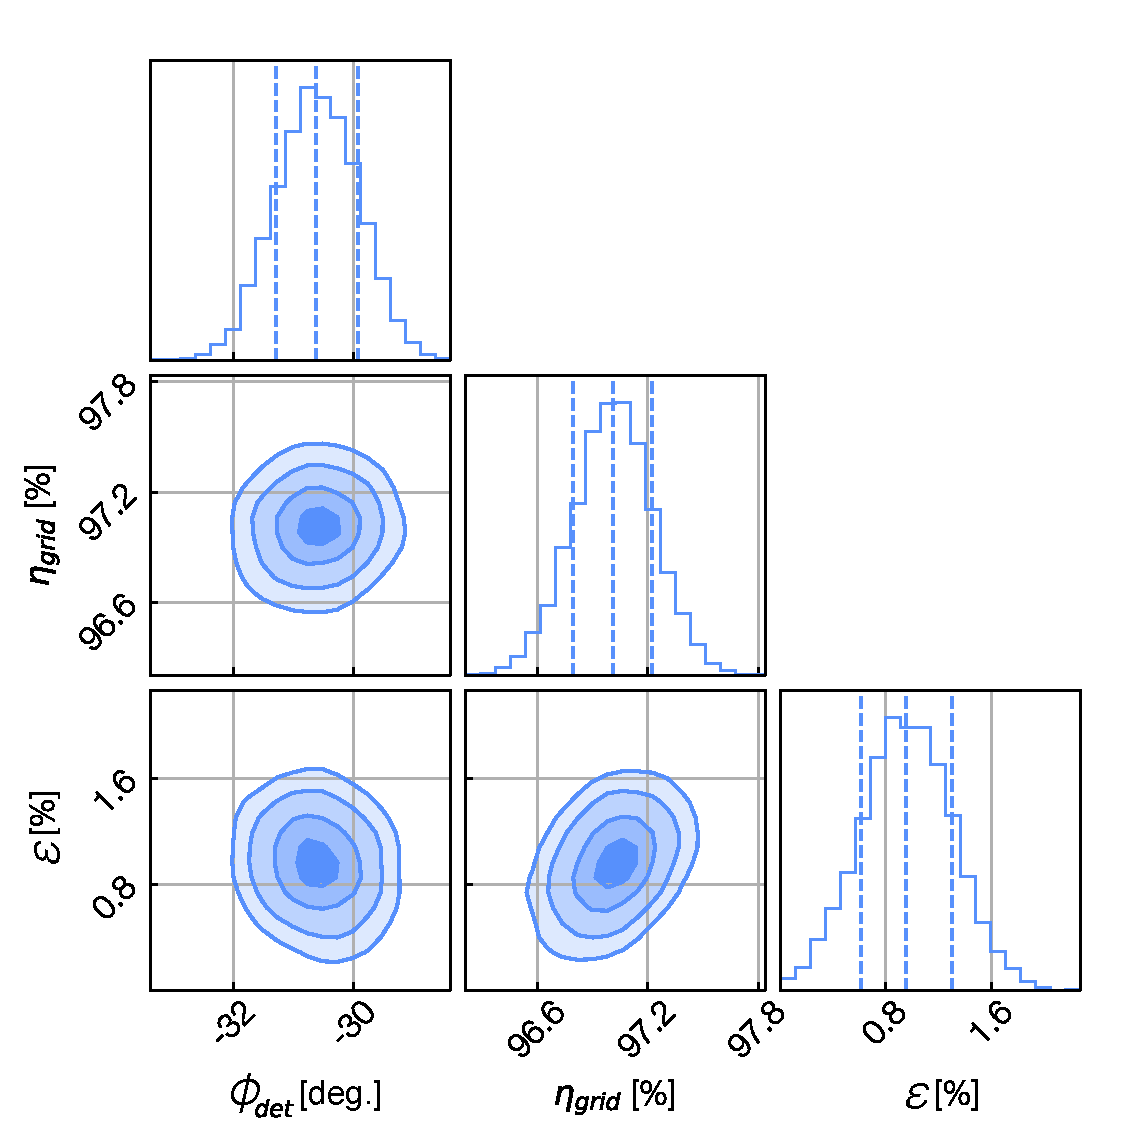
\includegraphics[height = .4\textwidth]{Figures/holo_crosspol_params.pdf}
    \caption{Left: Constrained parameters from polarization model (Eq.~\ref{eq:holo_model}), detector angle $\theta_{\text{det}}$, grid efficiency $\eta_{\text{grid}}$, and cross polarization $CP$.  Right: Polarized beam power (band-averaged from 85-120\,GHz) as a function of grid rotation, measured with the holography setup described in Section~\ref{sec:latot_meas_method}.  Co-polarization\,(blue) holds the source waveguide aligned with the receiver orientation.  Cross-polarization\,(green) uses a $90^{\circ}$ waveguide to make the source aligned perpendicular to the receiver orientation.  The polarization model (Eq.~\ref{eq:holo_model}) is fit using an MCMC and with no instrument polarization.}
    \label{fig:holo_crosspol_params}
\end{figure*}

\section{Public Code}
\label{sec:solat_code}
Here, we describe the software used for the holography data acquisition and analysis, all of which are made public.  The software is two-fold; 1) the \verb|solat-optics| module for simulating the near- and far-fields of the LAT telescope from the LATRt holography measurements and 2) Open Source Holography: a website detailing software and hardware to replicate the holography measurements.

\subsection{Optics Simulation}
The \verb|solat-optics| code includes several modules: beam simulation of the LATR optics tube, propagation of measured fields to the secondary mirror, and to the far-field (dependencies:~\cite{2020NumPy-Array,2020SciPy-NMeth,hunter2007matplotlib,reback2020pandas,mpiPython,tqdm}).  This beam simulation includes the lens geometry and computes the beam in the near-field.  The code can be adapted to produce the beam as a function of angle, as was used in this paper, or as a function of position in the measurement plane.  

The propagation analysis code inverts complex beams either from simulations or holography data, corrects for near-field aberrations using ray tracing and returns the complex fields propagated to a desired plane, either near- or far-field.   Notebooks are provided to show how to compute a beam simulation, how to analyze a LATRt holography measurement, and how to propagate a measurement to a desired region.  We invite users to adapt this code to any applications they see fit, but ask that publications using this code cite this paper and that code derived from this work remain public.

\subsection{Open Source Holography}
We also provide an open-source holography GitHub website:  \verb|holog-exp|~\cite{holog-exp}.  The repository provides both hardware and software details for recreating the holography measurements in this paper, and details on how to adapt the setup for future experiments.  The scripts demonstrate how to correlate signals with the FPGA, program the synthesizers, and program the XY stages to produce a holography beam map.  Further details can be found in Appendix~\ref{app:holog}.

\section{Conclusion}
\label{sec:discussion}
Refractive holography enables the testing of optical performance prior to deployment, and propagating the measurements into the far-field to predict the beam of the telescope.  We have presented holography measurements of the SO LAT optics tube and analysis methods determining its optical performance, including open-source holography for repeating and adapting the experiment.  We further provide an open-source package for simulating near-field holography measurements and propagating the measurements into the far-field using FD. 

From these data, we characterize the optical performance of the LATR optics tube.  We compare near- and far-field measurements to simulations.  After propagating the beams to the plane of the LAT secondary mirror, we find sub-percent power spilled to 300\,K.  We further find the far-field measured beams to be 2.18(1.38) arcmin FWHM in the F90(F150) band.

We provide three open-source software packages.  The first developed for this work, (\verb|solat-optics|~\cite{holog_sim_model}), models the LATRt holography measurements and is customizable to include arbitrary optics and adaptable for other optics experiments.  The second, (\verb|holog-exp|~\cite{holog-exp}), details the hardware and data acquisition software required in this experiment.  And lastly, we publish the data and Python scripts for recreating all figures in this paper~\cite{knowledge}.

The approach demonstrated here is broadly applicable to the characterization of millimeter-wave optical systems.  The ability to characterize the optical performance and systematics of the optics tube allowed us to determine one source of spurious reflections, and avoid systematics during future observations.  

\chapter{The Simons Observatory: Characterizing the Small Aperture Telescope with Radio Holography}
\label{ch:sat_holo}
This chapter presents holography measurements of the Simons Observatory Small Aperture Telescope at the University of California, San Diego, and preliminary characterization of its optical performance.  This work was made possible by the collaboration of Tommy Alford, Kathleen Harrington and Jeff McMahon from the University of Chicago, Remington Gerras from the University of Southern California, and Joe Seibert, Tran, Tsan, JB LLoyd, Michael Randall, and Kam Arnold from the University of California, San Diego.

\section{Introduction}
The Simons Observatory (SO) will employ three Small Aperture Telescopes (SATs) to measure the largest angular scales visible from the Atacama Desert in Chile.  One SAT has an aperture diameter of 0.42\,m and will measure roughly 10\% of the sky with more than 300,000 bolometer detectors across the three SATs~\cite{2020SPIE11445E7LK}.  Among the three SAT's are three frequency bands -- each with 10,000 detectors: Low-Frequency (LF) bands are centered at 27 and 39\,GHz, Mid-Frequency (MF) bands are centered at 93 and 145\,GHz, and Ultra-High-Frequency (UHF) bands are centered at 225 and 280\,GHz

Mapping the three frequency bands will allow for the separation of the CMB from galactic foregrounds (sourced from synchrotron and dust radiation).  The primary goal of the SATs is to measure the primordial tensor-to-scalar ratio, $r$, to within $\sigma(r) = 0.003$, which is one of SO's many ambitious science goals~\cite{ali20}.  Another ambitious science goal is to characterize the tiny polarization signal of the CMB.  Primordial B-mode spectra peaks at $\ell\approx90$ (or roughly $2^{\circ}$), and therefore precision measurements at large angular scales are critical.

We present the laboratory testing of the MF Small Aperture Telescope using the technique of near-field radio holography.  ``Holography" refers to the measurement of the complex monochromatic electric field wavefront using the interference between a modulated and reference signal.  Radio holography takes advantage of the antenna theory relationship: the far-field radiation pattern of a reflector antenna is the Fourier Transformation of the field distribution in the aperture plane of the antenna~\cite{alma_holog}.

\begin{figure*}[t!]
    \centering
    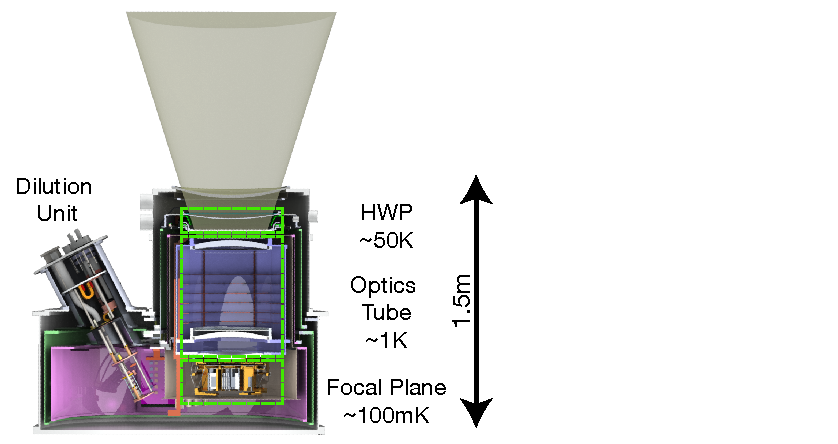
\includegraphics[width = \textwidth]{Figures/sat_optics.pdf}
    \caption{Left: Cross-section of the Small Aperture Telescope (SAT) optics tube.  Light enters through the high-density polyethylene window (UHMWPE) and through the cryogenic half-wave plate (CHWP).  The lenses re-image the beam onto the focal plane, where the holography detector measures power and phase at a given source position.  Right: SAT cryostat used in holography testing (Photo credit: Remington Gerras).}
    \label{fig:sat_optics}
\end{figure*}

Near-field holography of the SAT maps the wavefront emerging from the cryostat.  Using Fresnel diffraction (FD)~\cite{Goodman2005-ne}, these measured fields can be propagated to determine the far-field beam pattern of the telescope fed by this feedhorn receiver.  Moreover, these beams are useful for the identification and mitigation of optical problems within the receiver (i.e. optical aberrations, focus, scattered power, etc.).  These measurements enable a detailed verification of system-level optical performance prior to the deployment of a receiver on a telescope.

In Section~\ref{sec:sat_optics_tube} we describe the optical design and components of the SO SAT optics tube.  In Section~\ref{sec:satot_meas_method} we describe the measurement approach including the cryogenic receiver (\ref{sec:sat_cryo_rec}) and holography hardware (\ref{sec:sat_meas_hardware}) required for measuring beam maps (full details can be found in Appendix~\ref{sec:appendix_hardware}).  In Section~\ref{sec:sat_results} we present the measured beam maps.   Section~\ref{sec:sat_prop_fields} discusses analysis methods to propagate the measured beams into the far-field using FD.  We conclude with a discussion of future applications of this approach in Section~\ref{sec:sat_discussion}.  
\section{SO Small Aperture Telescope Optics Tubes Design}
\label{sec:sat_optics_tube}

\begin{figure}[t!]
    \centering
    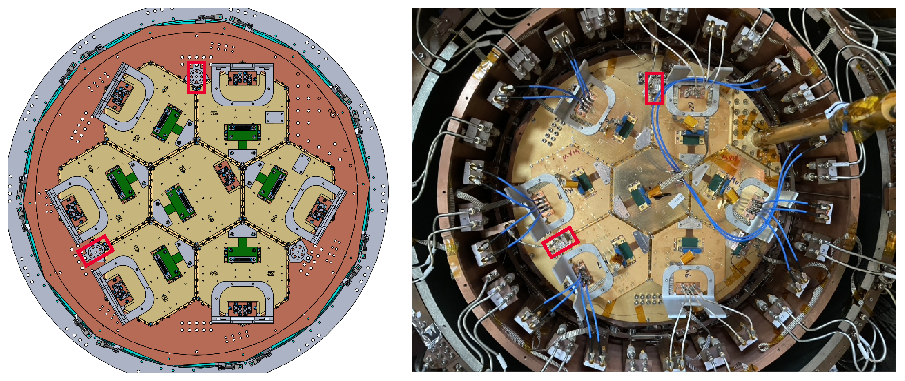
\includegraphics[width = \textwidth]{Figures/sat_fpa.pdf}
    \caption{SAT Focal Plane.  The two holography receivers are outlined in red, separated by $120^{\circ}$.  Two receivers are installed for redundancy, but also served as a useful tool when characterizing systematics (such as ``ghosting", or spurious signal in the beam maps, and polarization effects).}
    \label{fig:sat_fpa}
\end{figure}

Here we provide a brief overview of the SAT optics, starting at the window of the telescope and ending at the detectors.  The full SAT design is described in~\cite{ali20,2020SPIE11445E7LK} and shown in Figure~\ref{fig:sat_optics}.


Light enters through a 3\,mm thick ultra-high molecular weight polyethylene hexagonal window with an anti-reflection coating~\cite{zhu18}.  A Cryogenic Half-Wave Plate (CHWP) polarization modulator then reconstructs the polarization of the CMB at 40\,K.  For the duration of these holography measurements, the CHWP is held at a fixed angular orientation.  A 1\,K Lyot stop is the first cold optical element, and is followed by the SAT refractor.

The SAT optics is purely refractive; three anti-reflection coated silicon lenses~\cite{Datta:13,golec20} control the beam size and shape onto seven hexagonal detector arrays.  The SAT lenses are the largest Si lenses used for a CMB telescope to date~\cite{ali20}.  Baffles line in the inside of the SAT refractor to control spurious scattering.  Photons are then coupled onto the detectors by individual feedhorns. Seven hexagonal detector arrays are housed in the focal plane of the optics tube at 100\,mK.

\section{Measurement Approach}
\label{sec:satot_meas_method}
Here, we describe the hardware in two sections: 1) a cryogenic optics tube and 2) the holography system comprised of a source, correlation receiver, and motion system.
\subsection{Cryogenic System}
\label{sec:sat_cryo_rec}
The optics tube is housed in the SAT cryostat\cite{2020SPIE11445E7LK}.  The cryostat holds and cools the optics tube and provides support for detector readout.  This setup supports up to seven detector arrays (Fig.~\ref{fig:sat_fpa}).   In the test configuration, all bolometric arrays~\cite{2022arXiv220104507H} are filled in the focal plane, and two holography feedhorns are added to the edges of the focal plane, each separated by $120^{\circ}$.

The holography detectors consist of a feedhorn  identical to that used for the bolometric detectors, but with standard wave guide flanges at the outputs. A receiver consisting of a round to rectangular wave guide transition and a harmonic mixer is attached to this feed array.  The mixer was designed to operate from 70-110\,GHz, but was found to operate satisfactorily up to 170\,GHz. For operational simplicity, we used this mixer over our full frequency range from 85-135\,GHz.

Two identical receivers are installed in the focal plane for redundancy.  Two 0-18\,GHz coaxial connections were made from the receiver to connectors at the cryostat wall.  These coaxes are heat sunk at various stages between the focal plane, which was operated at 4\,K while doing holography, and the 300\,K cryostat wall.  A separate cool down was used to measure the loss along these coaxial feed lines.  The loss  was found to be 23\,dB at the LO frequency (10-13\,GHz).  Accurate knowledge of the loss along the feed lines is critical for providing the correct amount of power to the mixers in the focal plane.  The loss at the interference frequencies (IF) (100\,MHz) is significantly lower and not critical to the function of this system.

\begin{figure}[t!]
    \centering
    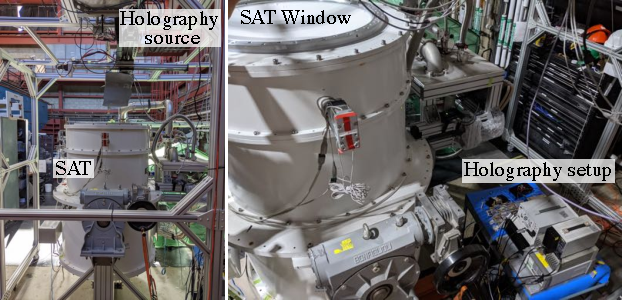
\includegraphics[width = \textwidth]{Figures/sat_exp.pdf}
    \caption{Lab photos of the holography setup on the SAT.  Left: The holography source, covered in a sheet of eccosorb to control scattering, is centered above the SAT window and points directly into the SAT, sitting below.  Right: The holography electronics sit on a cart next to the SAT readout.  The SAT window in the top left is made of UHMWPE.}
    \label{fig:sat_hardware}
\end{figure}

\subsection{Holography System}
\label{sec:sat_meas_hardware}

Figure~\ref{fig:setup} shows a schematic overview of the holography hardware.  Two millimeter-wave sources are used to measure the full SO MF band: F90 (80-120\,GHz) and F150 (130-170\,GHz).  Only one source is mounted at a given time.  The source is broadcast into the receiver using standard gain feed horns held close to the window ($\approx10$\,cm) (Figure~\ref{fig:sat_hardware}).

A motorized two-dimensional stage holds the source and is mounted on a support structure above the SAT.  During a measurement, the source (frequency is fixed) is moved over a $80\times80$\,cm range with 1\,cm steps.  One map takes roughly 2 hours to complete.

A common local oscillator (LO2 in Figure~\ref{fig:setup}) is fed to two harmonic mixers: 1) picked off from the source and 2) at the output of the cryogenic receiver.  The IF signal from both mixers in the 0-100\,MHz band is amplified and passed to a digital correlator (Casper ROACH2 ~\cite{roach2}) which computes the complex correlation between the two signals~\cite{ches18}.  The FPGA on the ROACH2 board outputs the amplitude and the phase of the correlated output, subdivided into a number of 100\,kHz wide bins.  Only the bin associated with the IF frequency is used in subsequent analysis.  The software to program and analyze output from the FPGA is made public on the \textit{McMahonCosmologyGroup} GitHub page in a package called \verb|holog-exp|~\cite{holog-exp}.  Appendix~\ref{app:holog} provides further details on the hardware of the holography setup.

Due to the presence of the CHWP, the source's polarized signal is modulated upon entering the optics tube.  Therefore, to understand the effects of the CHWP, we measure two beam maps at each frequency: with a waveguide twist at the output of the source, and without a waveguide twist.  This allows us to measure the response of the optics tube at two source polarizations (the waveguide twist changes the source polarization by $90^{\circ}$).

 \begin{figure}[t!]
    \centering
    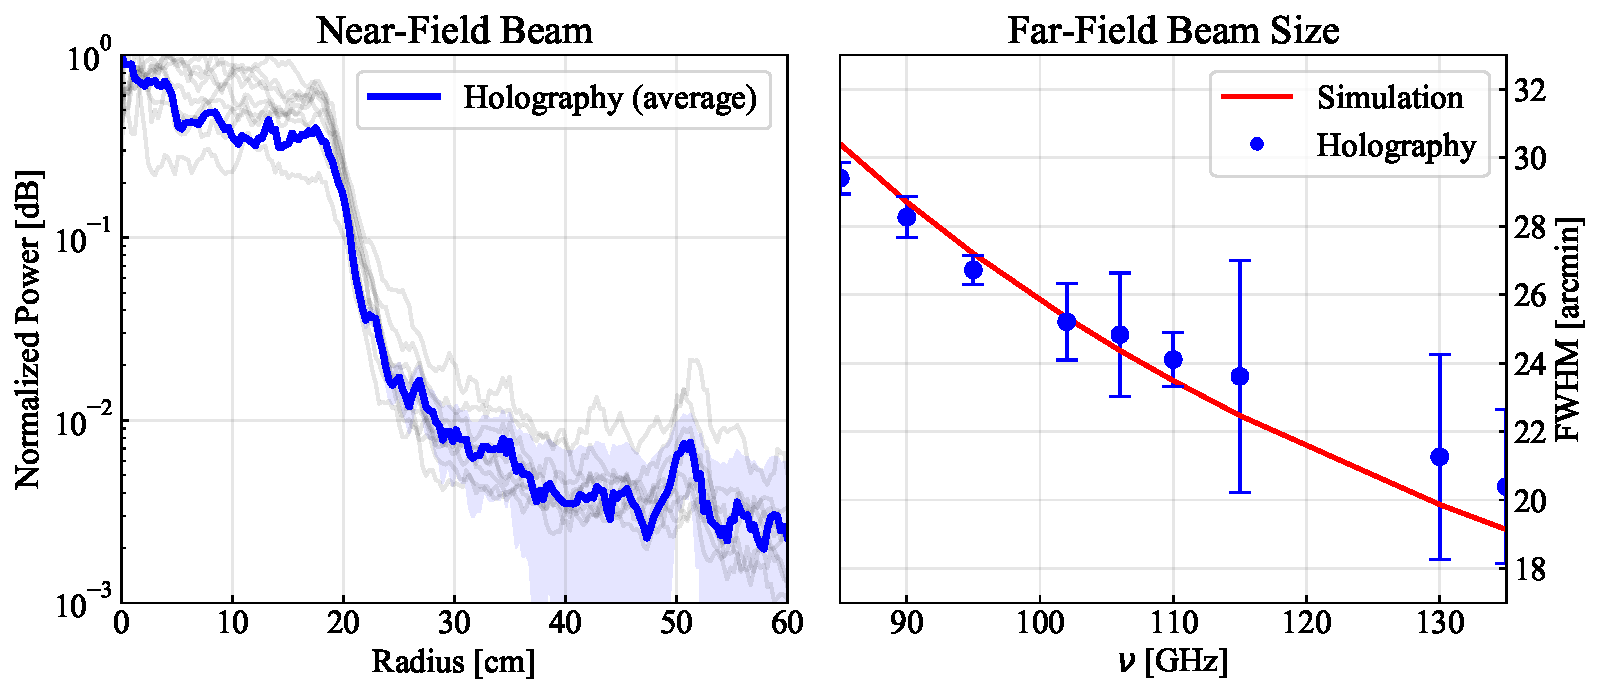
\includegraphics[width =\textwidth]{Figures/SAT_MF1_beam.pdf}
    \caption{Left: Preliminary near-field beam shape of the SAT in MF-1.  Beams are averaged over all frequencies measured, and the averaged beam is then radially averaged to get the near-field beam profile.  Right: Preliminary beam sizes of the SO SAT in MF-1.  Far-field beams measured with holography (blue) are radially binned and the FWHM is obtained from the resulting 1D beam profile.  Simulations are obtained using a diffractive optics simulation, and plotted are where the measured beam sizes with $2\sigma$ errorbars.}
    \label{fig:sat_fwhm}
\end{figure}

\section{Results and Interpretation}
\label{sec:sat_results}

\subsection{Near-Field Beam Maps}
Figure~\ref{fig:sat_mf_cobeam} and ~\ref{fig:sat_mf_crbeam} show the measured power and phase of the beam maps, respectively, at each frequency.   A variable attenuator at the output of the source was used to optimize the amount of signal entering the optics tube, to ensure power was not too high such that the measurement was saturated, but to also ensure the signal was high enough for signal-to-noise greater than 35\,dB.

Each beam map is labeled either $0^{\circ}$ WG, with a straight waveguide at the source output, or $90^{\circ}$ WG, with a waveguide twist at the source output.  These labels also correspond to the $E_x$ and $E_y$ fields.  We assume the source and receiver to be misaligned; to account for this, we rotate the two beams by $\theta$ which is fit to minimize $E_y^{'}$:

\begin{equation}
\begin{bmatrix}
 E_x^{'} \\
 E_y^{'}
 \end{bmatrix} = 
\begin{bmatrix}
 \cos(\theta) & \sin(\theta) \\
 -\sin(\theta) & \cos(\theta)
 \end{bmatrix}
\begin{bmatrix}
 E_x \\
 E_y
 \end{bmatrix}
 \end{equation}
 
The shape of the main beam was found to be in good agreement with simulations at all frequencies (Figure~\ref{fig:sat_fwhm}).  The phase measurement indicates the direction of the beam as it exits the window.  Figures~\ref{fig:sat_mf_cophase} and ~\ref{fig:sat_mf_crphase} shows the phases across all frequencies; the unwrapped phase is a gradient due to the beam exiting the window at an angle (as the holography detector is far-off from bore sight in the focal plane).  However, we further note the change in phase gradient as a function of frequency and have modeled this to be an aliasing effect of the measurement.  The aliasing effect creates a directional shift in the on-sky beam, but is negligible for determining the on-sky beam size.

 \begin{figure*}[t!]
    \centering
    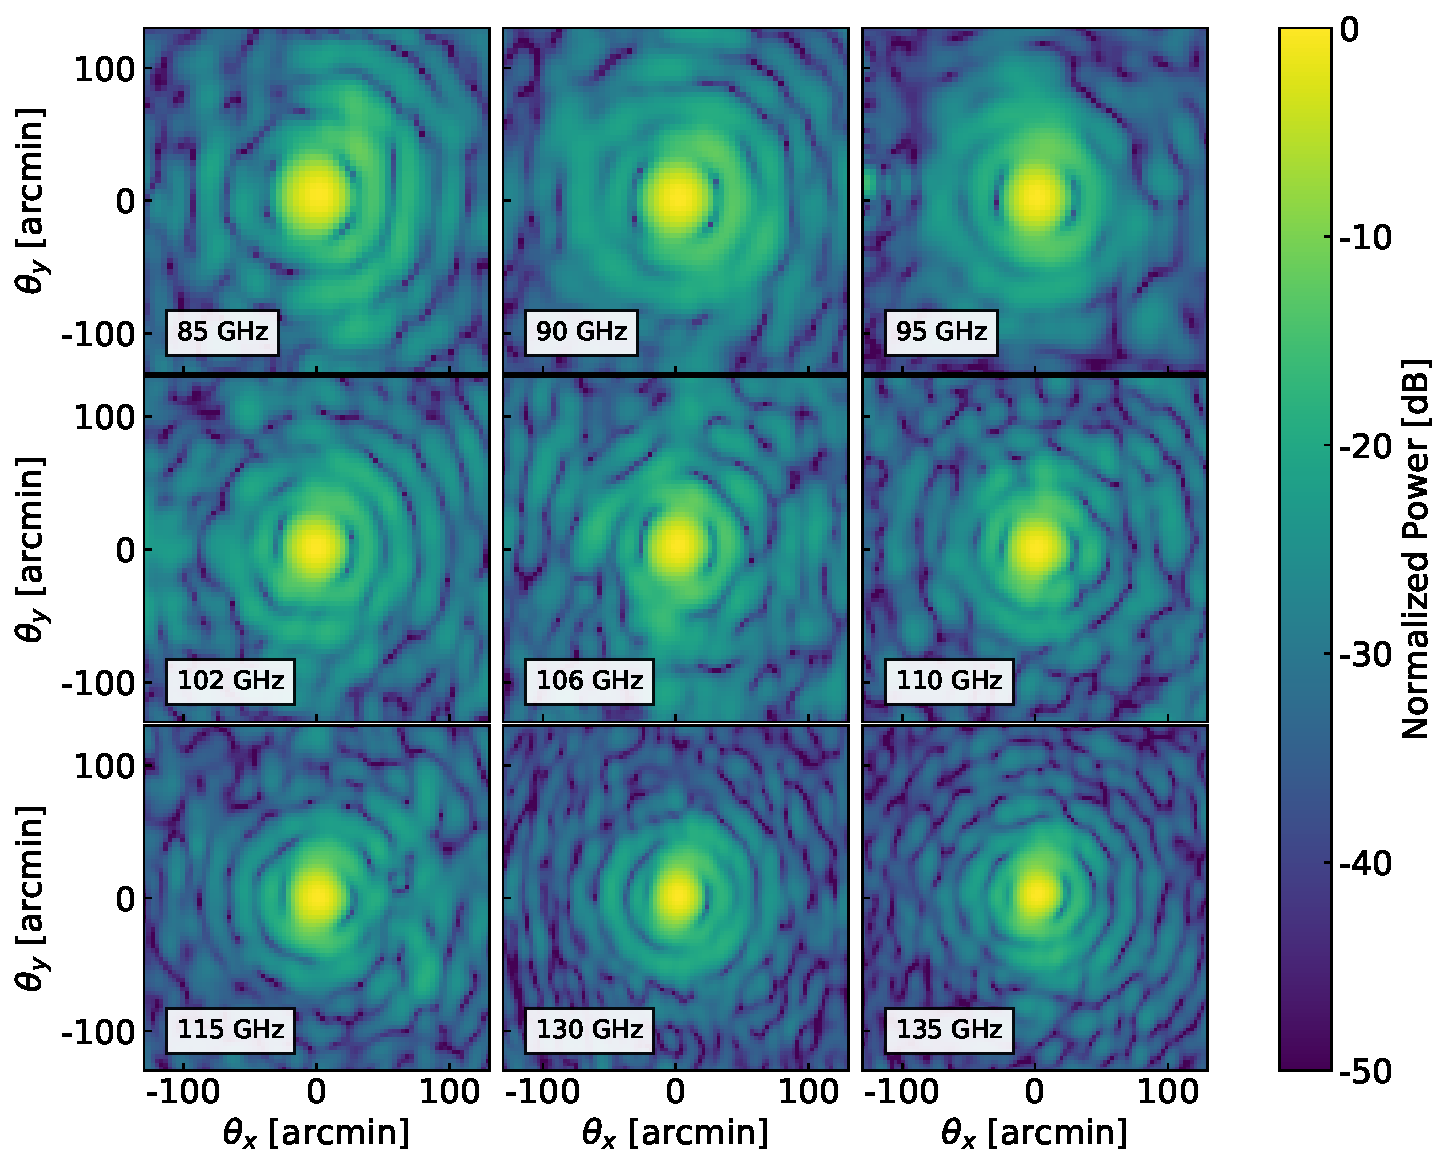
\includegraphics[width = \textwidth]{Figures/farfield_sat.pdf}
    \caption{Preliminary far-fields of the SAT optics tube in the MF-1.  The near-field measured beam is propagated to the far-field for each frequency.  The aliasing of the measured phase in the near-field (discussed in Section~\ref{sec:sat_results}) caused an artificial directional shift in the on-sky beam, which we center before plotting.}
    \label{fig:farfields_sat}
\end{figure*}

\subsection{Propagation of Fields}
\label{sec:sat_prop_fields}

The performance of the SAT optical system is assessed in detail by using the amplitude and phase of the measured beams to calculate the far-field.  This is carried out by using the Fourier relationship between the near-field $E(x,y)$ and far-field $B(\theta_x,\theta_y)$ beams \cite{McIntosh2016,alma_holog}:
\begin{equation}
    B(\theta_x,\theta_y) = \int_{\text{aperture}} E(x,y) e^{ i \frac{2\pi}{\lambda} (\theta_x x + \theta_y y )} dx \, dy 
\end{equation}
where the complex electric field $E(x,y)$ is integrated over the area of the aperture, $\theta_x$ and $\theta_y$ are the on-sky angular coordinates, and $\lambda$ is the wavelength.  

The resulting (preliminary) far-fields are shown in Figure~\ref{fig:farfields_sat}.  The measured beam size $26.02^{\prime}\pm YYY^{\prime}$ is consistent with the predicted F90 FWHM of $24.95^{\prime}$.

\section{Discussion}
\label{sec:sat_discussion}

We have presented holography measurements of the SO SAT optics tube and analysis methods determining its optical performance.  We further provide an open-source package for simulating near-field holography measurements and propagating the measurements into the far-field using Fourier optics.  From these data, we characterize the optical performance of the SAT MF optics tube.  We compare near- and far-field measurements to simulations.  After propagating the beams to the far-field, we find the SAT beam FWHM to be ($26.02^{\prime}\pm YYY^{\prime}$) in the F90 band, within the expected beam size of $24.95^{\prime}$, and is sufficient to accomplish SO's science goals at these angular scales.

We also provide \verb|sosat-optics|, an open-source software package, which models the SAT holography measurements and is customizable to include arbitrary optics and adaptable for other optics experiments~\cite{sat_sim_model}.  The approach demonstrated here follows the successful characterization of the Large Aperture Telescope Receiver tester, and is broadly applicable to other millimeter-wave optical systems~\cite{chesmore2022}.  The ability to characterize the optical performance and systematics of the optics tube allowed us to determine the SAT optics is in focus and that the beam is within requirement for SO science. 

\begin{figure}
    \centering
    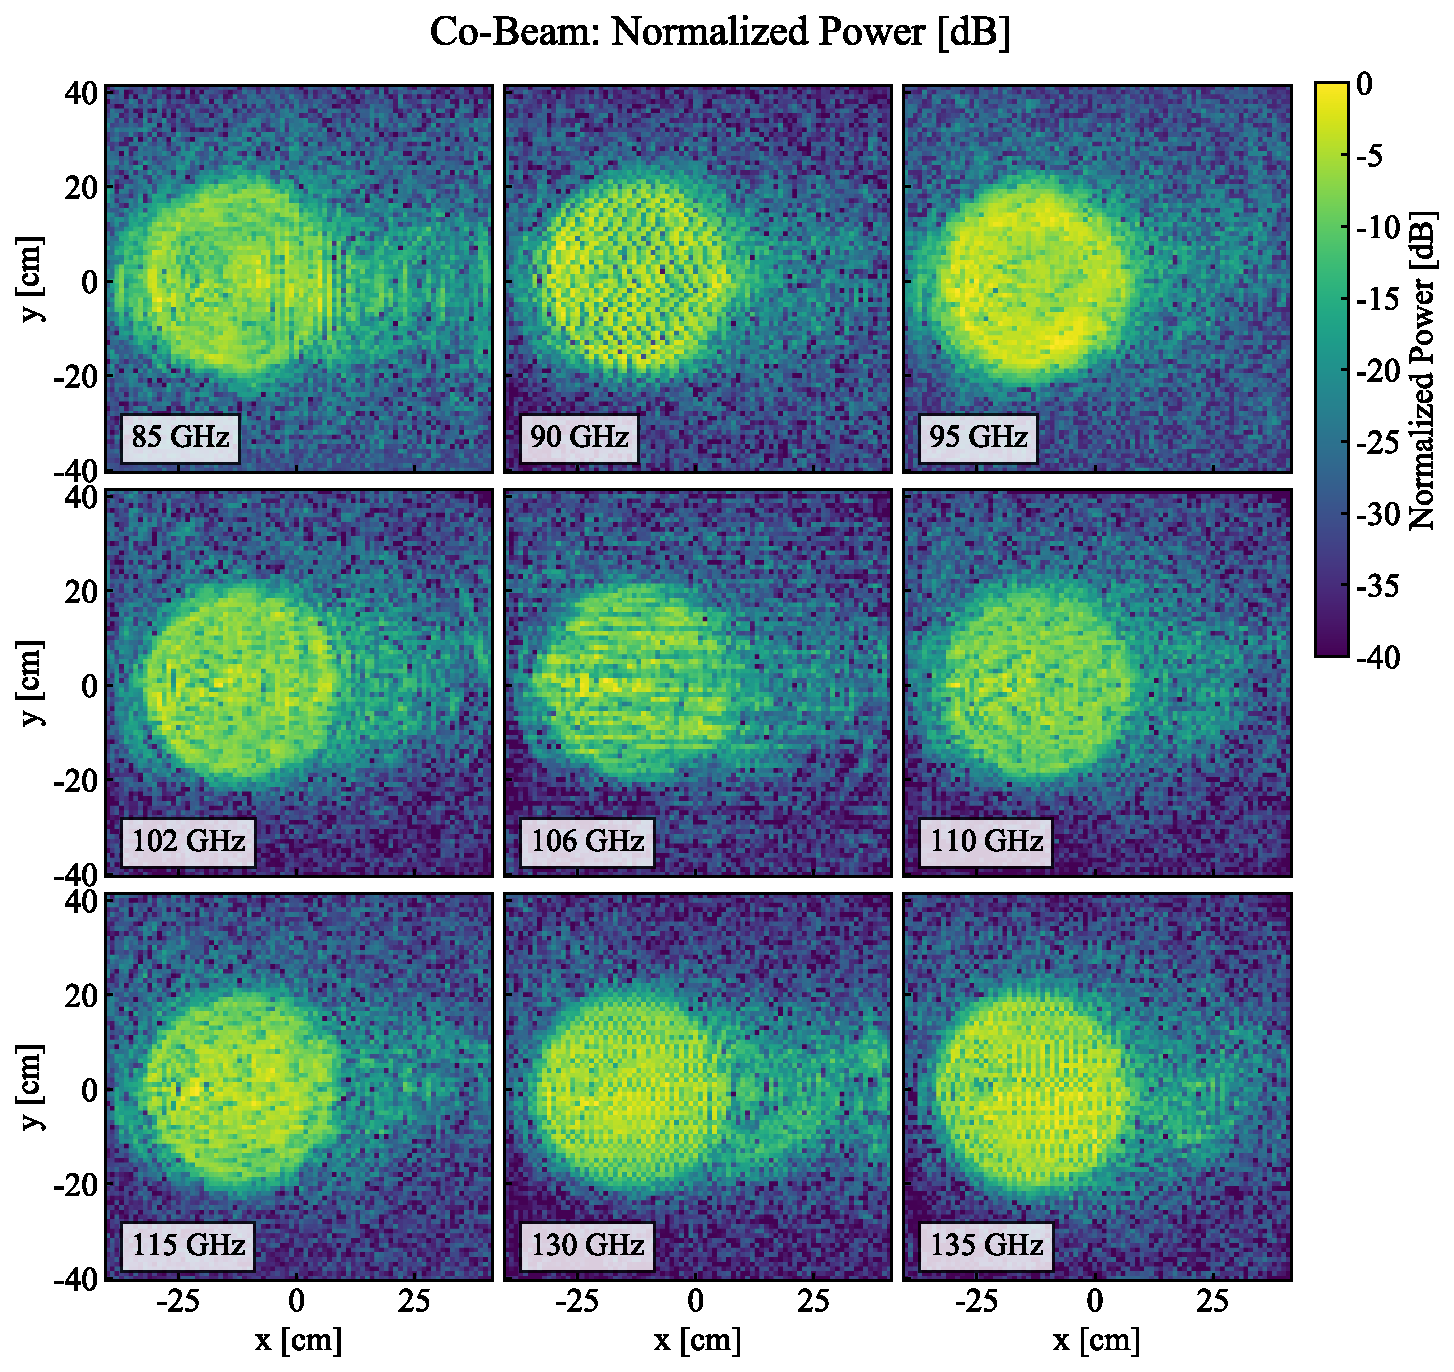
\includegraphics[width = \textwidth]{Figures/SAT_MF1_co-beam.pdf}
    \caption{Co-polar normalized power of the Simons Observatory Small Aperture Telescope near-field beam.}
    \label{fig:sat_mf_cobeam}
\end{figure}

\begin{figure}
    \centering
    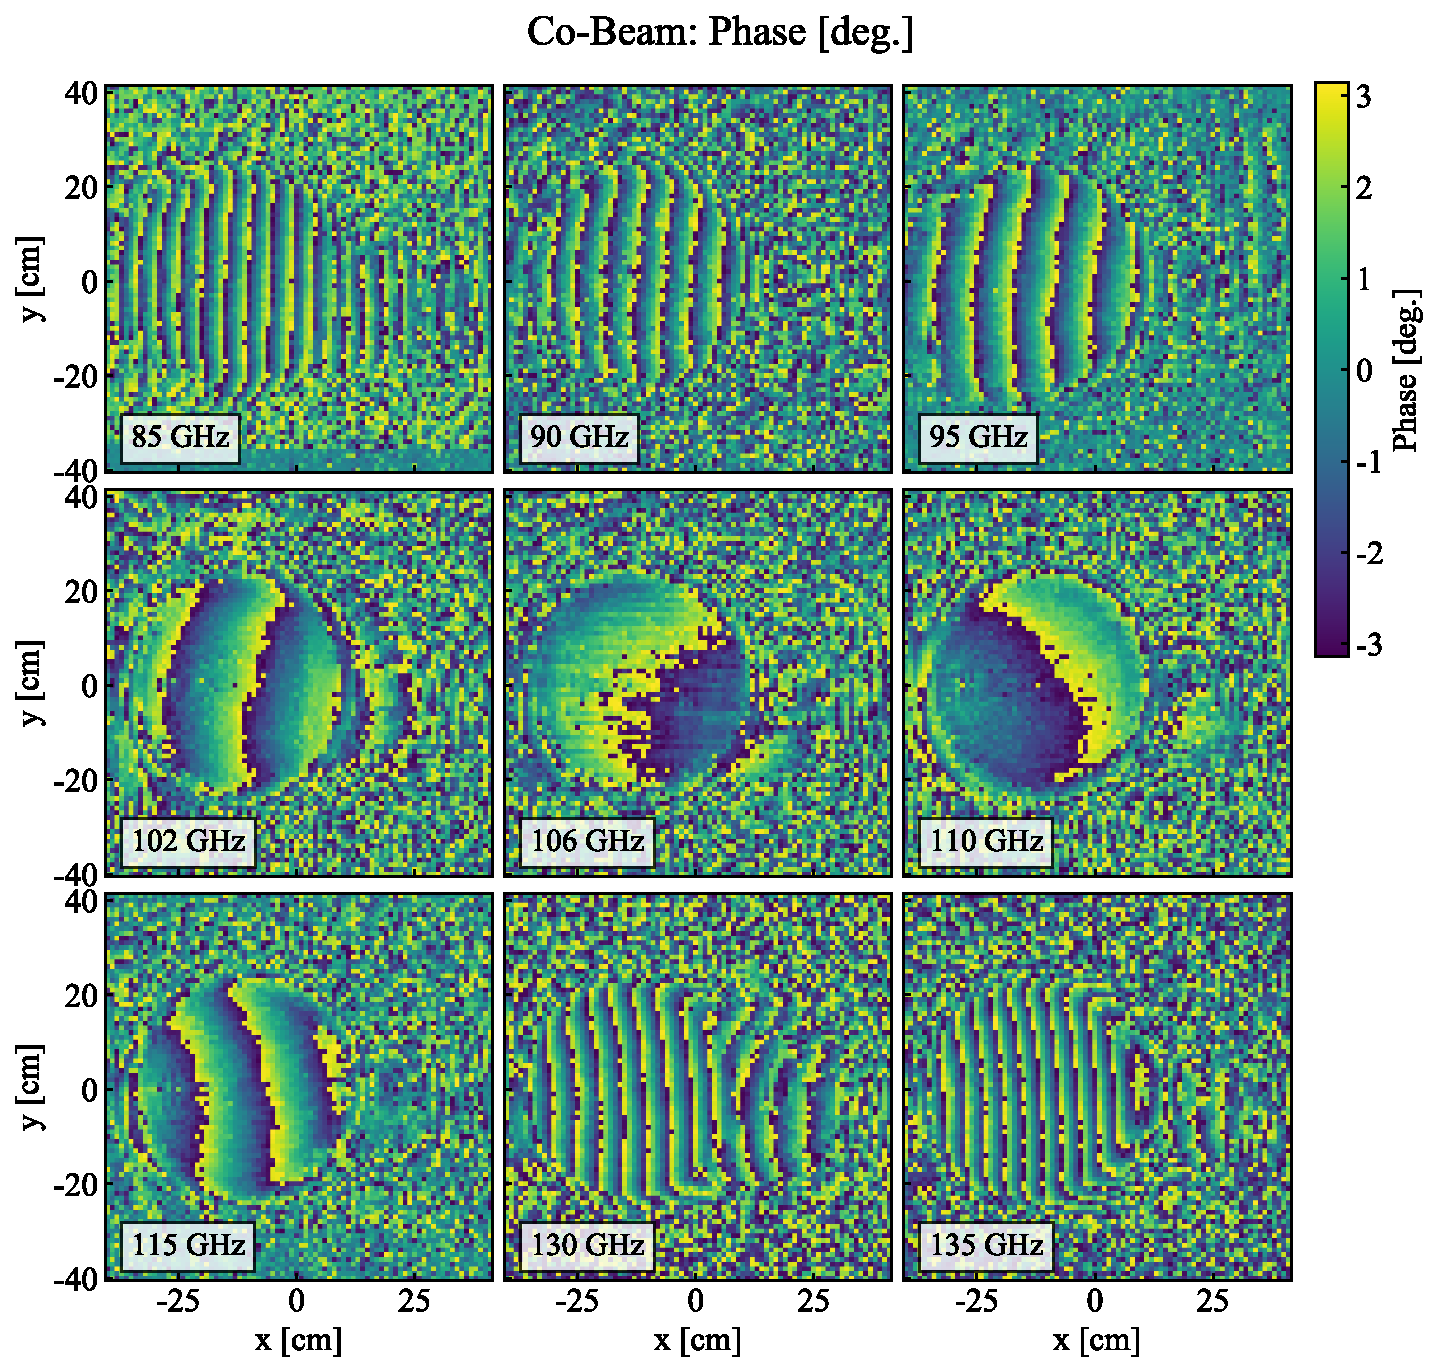
\includegraphics[width = \textwidth]{Figures/SAT_MF1_co-phase.pdf}
    \caption{Co-polar phase of the Simons Observatory Small Aperture Telescope near-field beam.}
    \label{fig:sat_mf_cophase}
\end{figure}

\begin{figure}
    \centering
    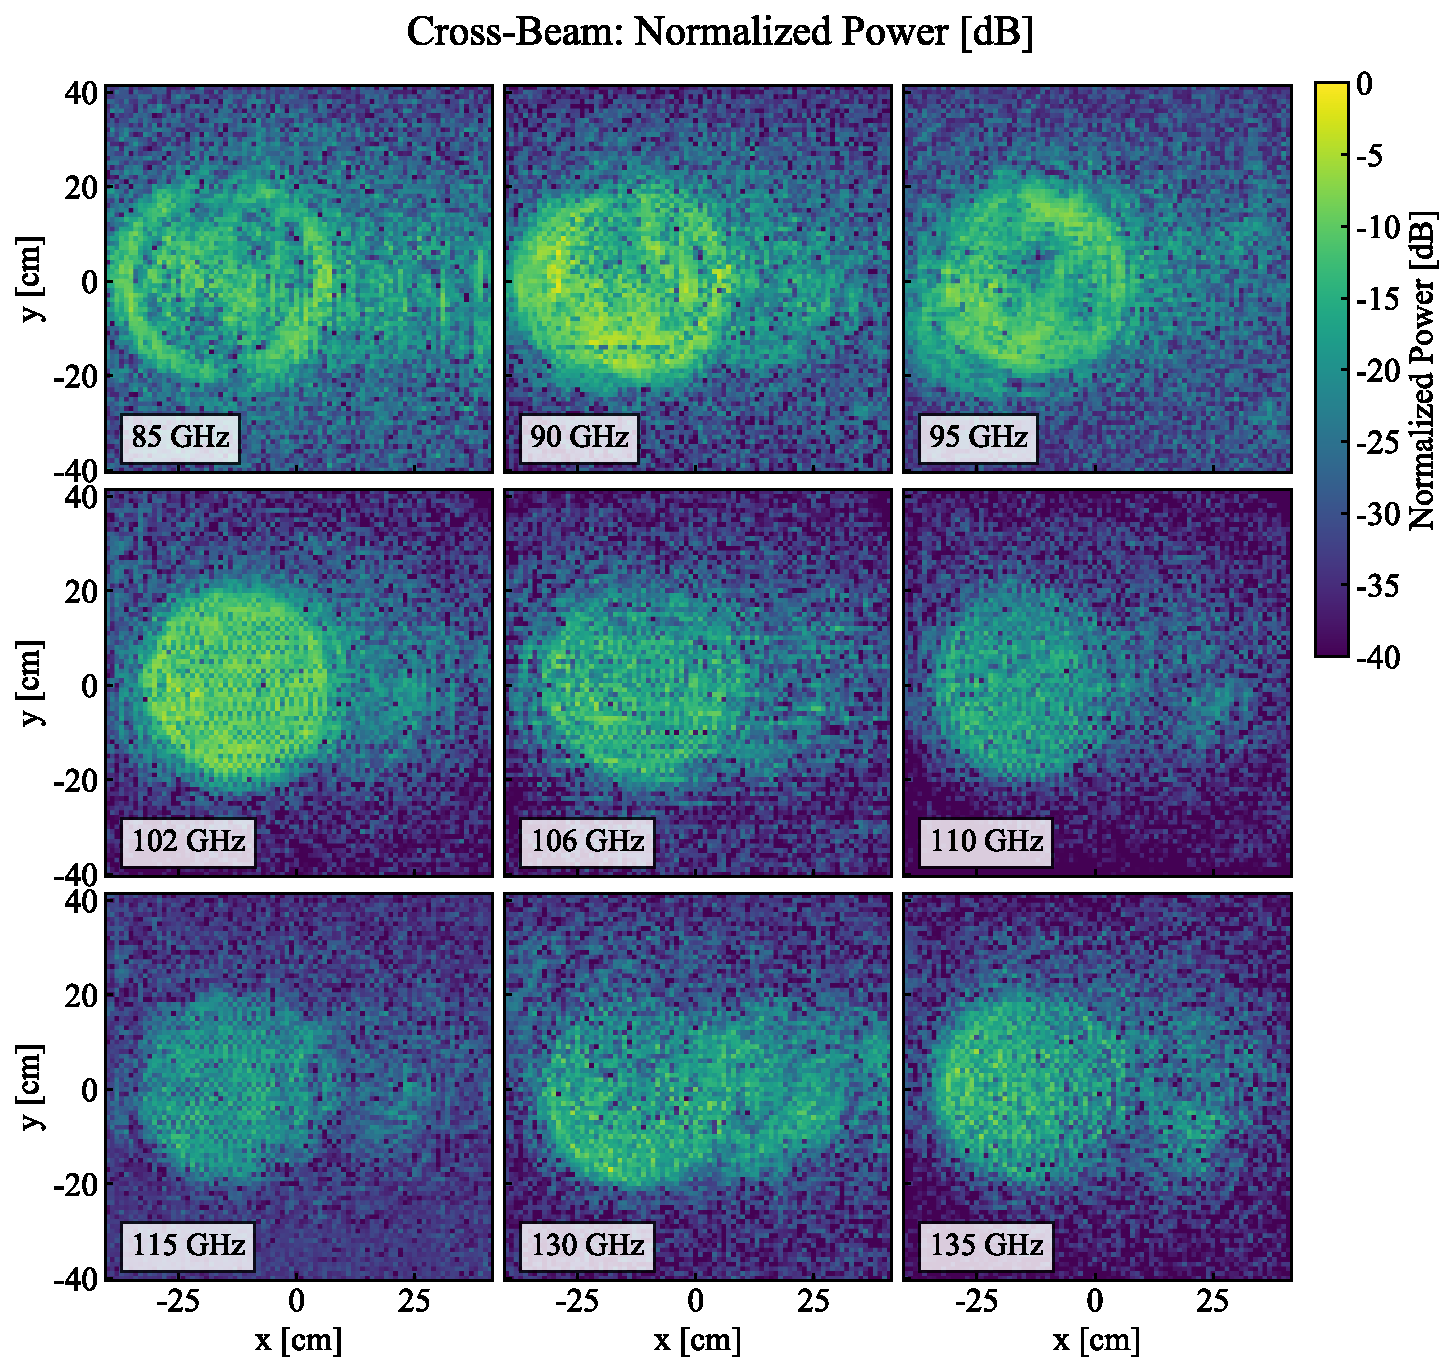
\includegraphics[width = \textwidth]{Figures/SAT_MF1_cr-beam.pdf}
    \caption{Cross-polar normalized power of the Simons Observatory Small Aperture Telescope near-field beam.}
    \label{fig:sat_mf_crbeam}
\end{figure}

\begin{figure}
    \centering
    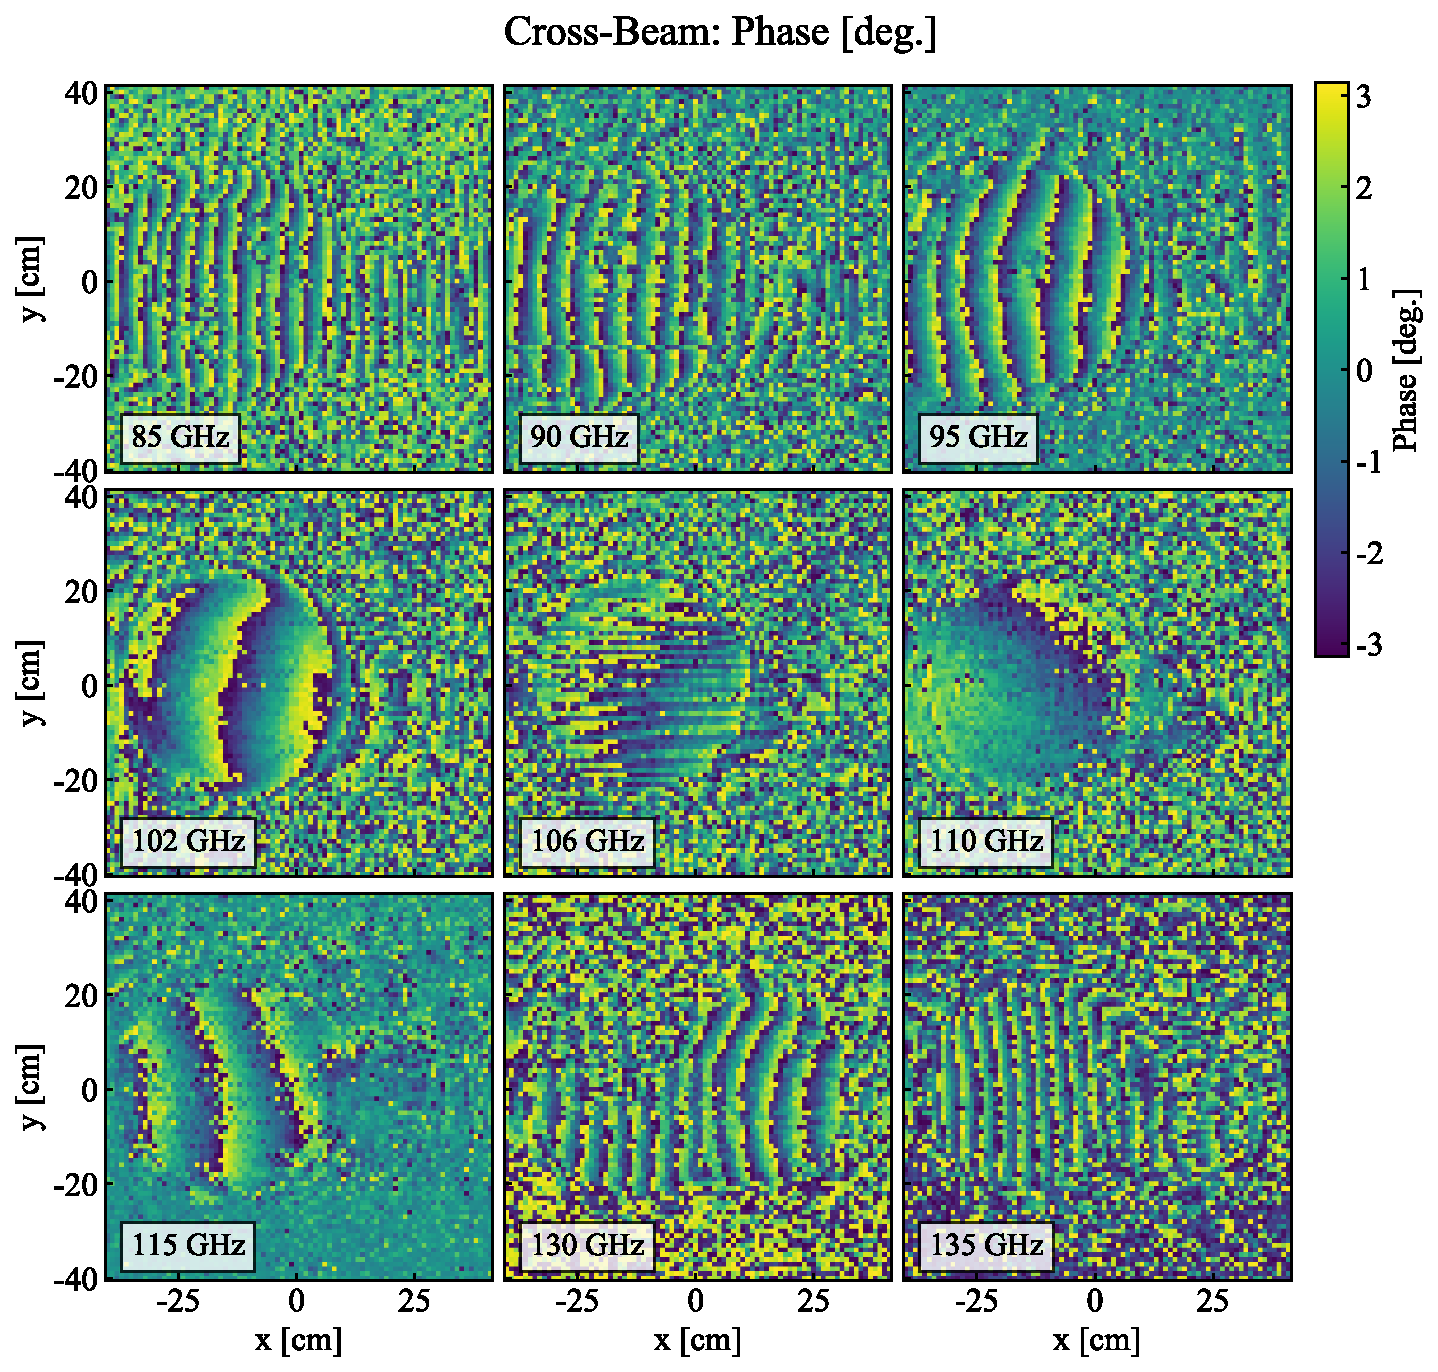
\includegraphics[width = \textwidth]{Figures/SAT_MF1_cr-phase.pdf}
    \caption{Cross-polar phase of the Simons Observatory Small Aperture Telescope near-field beam.}
    \label{fig:sat_mf_crphase}
\end{figure}

\chapter{HoloSim-ML: machine learning applied to the efficient analysis of radio holography measurements of complex optical systems}
\label{ch:holosim}
\section{Introduction}
Simons Observatory (SO) is an ensemble of millimeter-wave telescopes which will observe the cosmic microwave background (CMB) temperature and polarization signals~\cite{gali18, so19}. SO comprises one Large Aperture Telescope (LAT)~\cite{Niemack:16, Gudmundsson:21,Parshley_2018} and three Small Aperture Telescopes (SAT)~\cite{ali20} which together will measure the temperature and polarization anisotropy of the CMB from several degrees to arc-minute angular scales.

The science goals of SO require high sensitivity and tight control over systematic errors.  Since the sensitivity of state of the art millimeter-wave receivers is limited by photon noise from background radiation, improvements in sensitivity for a given instrument require careful control over every part of the instrument.  Deviations of the mirror surface will redistribute beam power to large angular scales and therefore increase the width of the main beam and reduce the forward gain of the telescope.  In this work we focus on quantifying these effects, and we present the tools needed to mitigate them by aligning the mirror panels of the LAT using holography.

The LAT is a crossed-Dragone telescope~\cite{6773968,Gudmundsson:21,Niemack:16,2021RNAAS...5..100X} developed in collaboration with the Cerro Chajnantor Atacama Telescope prime (CCAT-prime)~\cite{ccat,aravena2019ccatprime} Collaboration.  The LAT design is shown in Figure~\ref{fig:lat}.  The telescope is engineered and built by Vertex Antennentechnik GmbH, the panels forming the primary and secondary mirrors, both 6 m in diameter, were fabricated by Bricon Technology GmbH~\cite{vertex}.  A defining feature of this design is the large focal plane (2\,m in diameter) that can accommodate more than 70,000 detectors for CMB studies~\cite{Parshley_2018,zhu2021simons,mccarrick2021simons}. The primary\,(secondary) mirror is built with 77\,(69) panels, and has 385\,(345) adjusters in total.  The size of each panel is roughly half a square meter and weighs roughly 5\,kg~\cite{ccat}.  An adjuster is a threaded mechanism allowing for manual adjustment of the position of each panel~\cite{Woody}.  Each panel has five adjusters controlling the surface height.  We present radio holography tools that allow us to reach a combined reflector surface error of $22\,\mu$m RMS or less.

Radio holography has a long history of use in millimeter and sub-millimeter telescopes~\cite{alma_holog,Sridharan,7228408,5722985,morris:1143663,Fienup:93}.  Typically, these applications require aligning a single mirror, which can be measured in isolation~\cite{1141354,Hunter2011}.  A particular challenge of this application is that we must measure both mirrors simultaneously and then extract the adjuster errors from each of the two mirrors.  This complex optical system requires the development of new fitting tools for efficient analysis.  Towards this end, we developed an efficient simulation code and used it to train a machine learning (ML) model to do this extraction.
Practical holography measurements of telescopes of this size must be carried out with a bright monochromatic source in the near-field.  The analysis of near-field holography is described in great detail in several references~\cite{alma_holog,5722985,1190}.  The CCAT-prime Collaboration carried out a parallel work simultaneously with ours, which details measurement methods \cite{fyst_holog}.  The method described is commonly referred to as “near-field vector beam mapping” and employs a coherent source and phase sensitive receivers.  For a given desired accuracy, this requires a lower signal-to-noise than Out-of-Focus Holography (OFH), which reconstructs the telescope aperture phase through comparison of far-field power maps taken in and out of focus with a coherent source and incoherent detectors in the focal plane~\cite{Serabyn:91}.  In this work, we examine the impact of mirror alignment on measurements of the CMB, explore the sampling of the focal plane required to arrive at a given mirror RMS, and  present a new approach to fitting complex optical systems that we expect to be far more general than the present example.

In Section~\ref{sec:motive} we quantify the scientific impact of improving the mirror surface.  In Section~\ref{sec:simulate} we describe the simulations we use to model these holography measurements.  In Section~\ref{sec:method_align} we describe our analysis of near field holography data using ray-tracing to determine the near field corrections.  In Section~\ref{sec:ml} we describe how we use these simulations to train a machine learning code to efficiently and accurately extract the adjuster errors from holography data.  We discuss how the number of measurement positions impacts the remaining degeneracies in the panel errors.  In Section~\ref{sec:meas_method} we explain the method for performing this measurement, including hardware tolerances and alignment.  Section~\ref{sec:code} details the publicly available code.  We conclude with a discussion of other potential applications in Section~\ref{sec:holosim_conclusion}.  
\section{Motivation}
\label{sec:motive}

Measurements of the CMB are typically expressed as power spectra computed from all-sky maps using the spherical harmonic transform.  Therefore, the impact of the scattering of power due to mirror surface deviations can be understood by transforming these beams into $\ell$-space window functions.  These window functions encode how the beam shape rolls off the CMB power spectrum as a function of $\ell \sim 180^\circ / \theta$.  This transformation is equivalent, in the flat sky limit, to Fourier transforming the beam and averaging its magnitude squared in bins of constant wave number.  For reference, $\ell = 1000$ corresponds to an angular scale of $0.18^\circ$.

\begin{figure}[t]
    \centering
    \includegraphics[width = .7\textwidth]{Figures/far_field_win_func2.pdf}
    \caption{Top: Far-field beam simulation of a 150 GHz source, with surface error RMS of $0\,\mu$m, $20\,\mu$m, $35\,\mu$m, and $50\,\mu$m. The side-lobes around the central beam increase as RMS of panel errors increases. Center: Window function $W_\ell$ of far-field beams at 150 GHz with combined surface RMS of $50\,\mu$m, $35\,\mu$m, $20\,\mu$m, and $0\,\mu$m. Bottom: Difference of window functions $W_\ell$ in top plot, w.r.t. window function of far-field beam with surface error RMS of $0\,\mu$m, $W_{\ell,0\mu}$.}
    \label{fig:win_func}
\end{figure}
The upper panels of figure~\ref{fig:win_func} show simulations of the LAT beam pattern with varying levels of panel setting errors at 150 GHz, one of our key science bands.  These simulations were generated using the method described in Section~\ref{sec:simulate} in the far-field.  We note that the calculation extends to a larger angle, but we have truncated it in the figure for clarity of presentation.  It is apparent that the panel errors lead to significant scattering of light from the main beam into near side-lobes.

The plots of Figure~\ref{fig:win_func} display these window functions for the simulated beams (top row) and the difference between the window functions with panel errors and that of a perfect mirror (bottom).  For reference, the vendor will deliver the telescope mirrors with a half-wave front error (HWFE) of $50\,\mu$m.  The current method of panel alignment using a laser tracker achieved a surface error of the panels to $20-25\,\mu  m$ for the 6\,m primary mirror of the Atacama Cosmology Telescope~\cite{act_inst}.  The surface error budget for the SO LAT give a $35\,\mu$m HWFE if similar panel errors are achieved.  This leads to a 10\% loss in signal in the $1000<\ell < 5000$ range that is crucial for much of the SO science~\cite{so_science}.  This matches the prediction of the Ruze formula~\cite{ruze} once one accounts for the fact that the power spectrum (and window function) are proportional to the square of the beam.  Since the calibration of the power spectrum is based on cross-correlating with data from the Planck Satellite~\cite{planck_data} for $\ell \lesssim 1600$, the variation in the window function in this range represents a potential systematic challenge.  Reducing the half-wave front error to below 22 $\mu$m would simplify calibration and recover most of this lost sensitivity.  The error budget for our telescope shows that this requires measuring and setting each of the primary and secondary mirror to an accuracy of better than $5 \mu$m RMS, which we take as a goal for this work.

\section{Beam Simulation}
\label{sec:simulate}
The SO LAT is shown in Figure~\ref{fig:lat} and described in~\cite{2021RNAAS...5..100X}.  We compute its beam pattern in the near-field and far-field using physical optics~\cite{hecht,Gudmundsson:21} implemented in a code we call \verb|HoloSim-ML|, available at GitHub.com/McMahonCosmologyLab~\cite{McMahonCosmologyLab}.

\begin{figure}
    \centering
    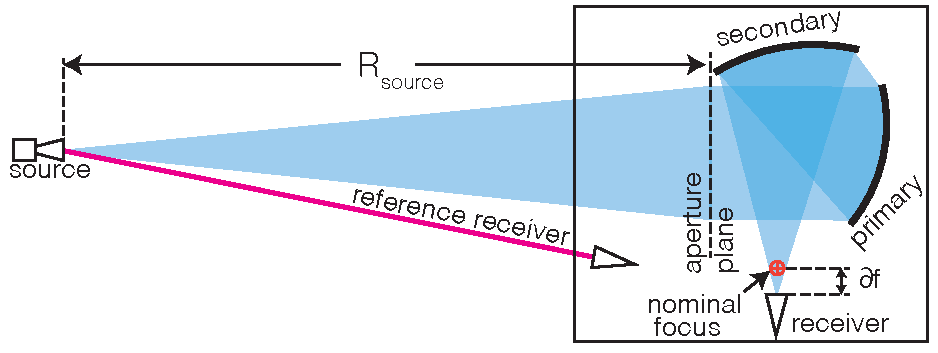
\includegraphics[width = .9\textwidth]{Figures/holography_geo3.pdf}
    \caption{Holography geometry. A source on a 5\,m tower sits at a distance $ R_{\text{source}}$ above the aperture plane of the LAT. Two receivers, one "reference" receiver pointed straight at the source, and the receiver in the focal plane, measure the amplitude and phase of the source. The focal plane receiver is offset $\delta f$ from the nominal focus.}
    \label{fig:hologeo}
\end{figure}

A two-dimensional representation of the three-dimensional geometry used in these simulations is shown in Figure~\ref{fig:hologeo}.  We specify the positions and rotational state of the mirrors, the location of the receiver feed, and the location of the source.  For these simulations, we refocus the telescope on the near-field source by displacing the receiver a distance $\delta f$ from the nominal telescope focus. We ray-trace from a receiver position through the telescope to an aperture plane chosen at an arbitrary position a few meters in front of the telescope. The results do not depend on this arbitrary choice.  Each ray is given an amplitude based on a modeled beam pattern for the receiver feed horn.  A reference receiver, placed outside the telescope, points directly at the source and, in combination with the receiver feed, determines the phase of the source.  For the results presented here, the beam width of the receiver feed was assumed to be $44^\circ$ with a Gaussian profile.  We typically use a 100\,x\,100 grid of points on the aperture plane. This telescope model is rotated, and this calculation is repeated for every azimuth and elevation pointing to simulate the two-dimensional diffraction pattern.

To model misalignment of the mirrors, the surface $z_{surf}$ of each mirror panel, is parameterized as a polynomial function of the five parameters $a_n$:
\begin{equation}
     z_{\text{surf}} = a_1 + a_2 r_x+ a_3 r_y +a_4 (r_x^2 + r_y^2) + a_5 r_x r_y 
     \label{eq:zsurf}
\end{equation}
where $r_x$ and $r_y$ are coordinates centered in each individual panel.  The $a_n$ parameters are determined by fitting this equation to the surface offsets $\delta_z$ at the positions of the five mirror adjusters. Thus, there is a one-to-one mapping between adjuster offsets and the parameters in this model.  The surface machining errors for each panel will be a few micrometers and the adjuster system is the same as was used for SPT where a similar model was fit successfully \cite{Carlstrom_2011}.  Therefore, this panel model is expected to be adequate for these purposes.

\begin{figure}[t]
    \centering
    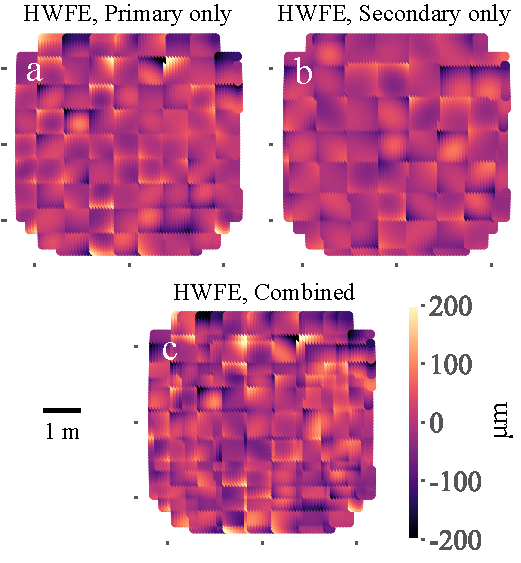
\includegraphics[width = .8\textwidth]{Figures/example_pathl_single_column2.pdf}
    \caption{Simulated HWFE at the aperture plane with surface errors of $35\,\mu$m RMS on a) only M1, b) only M2, and c) both M2 and M1.}
    \label{fig:pan_mod}
\end{figure}

The output of this step in the code is the amplitude and path length to the aperture plane from the receiver feed.  Figure~\ref{fig:pan_mod} shows the resulting variation in the path length across the aperture plane for one realization of panel errors from the primary mirror (left) to the secondary mirror (right) and the combination of both (bottom).  It is clear that the errors due to the secondary and primary mirror panel misalignments occur at slightly different physical positions and scales in the aperture plane.  This means that a single holography measurement may suffice to extract the panel errors. 

The next step in the calculation is to determine the straight line path length from each point in the aperture plane to a source.  The source is chosen to be at $R=1\times 10^6$\,m for the far-field and $R=1\times 10^3$\,m for near-field holography.  The elevation $\theta$ and cross-elevation $\phi$ of this source are varied to map out the beam.  This results in a total path length from the source to the receiver.  The beam $B(\theta,\phi)$ is then calculated using:
\begin{equation}
    B(\theta,\phi) = \sum_j E_j e^{i \rho_j(\theta,\phi) 2\pi/\lambda} 
\end{equation}
where $j$ is an index for the rays in the simulation, $E_j$ is the electric field amplitude of a ray, and $\rho_j(\theta,\phi)$ is the path-length from receiver through the telescope and to the source tower for a given pointing, and $\lambda$ is the wavelength.  We note that we can also compute the diffraction pattern in the aperture plane by fixing the source's position and varying the receiver position in the focal plane.  

\label{sec:method_align}
Radio holography consists of measuring the electric field amplitude and phase of the beam, and then utilizing the Fourier transform relationship between the aperture fields and beam to extract the fields and phase on the aperture plane.  In our case, variations in the phase of the aperture plane are interpreted as two times the errors in the mirror surface.

For practical reasons, and to reduce the impact of atmospheric turbulence, these measurements are usually carried out with a near-field transmitter.  This introduces de-focus and other geometrical aberrations that must be removed in order to interpret these data.  In previous analyses, these have been corrected by fitting out functional forms that capture these effects~\cite{alma_holog}.  Here we use our ray tracing code to model the aberrations by computing the phase on the aperture plane, including contributions internal to the telescope and between the telescope and the source.  This requires that we measure the position of the source and the position of the receiver.  After we apply this phase correction, we also remove a constant and gradients from the aperture fields to account for any small pointing errors.  This approach has been checked against the standard series expansion and generalizes easily to include additional corrections, including for the phase of the receiver feed horn.  The left panel of Figure~\ref{fig:ap_resids} shows the simulated holography measurement of SO that results from this calculation.

\section{Panel Fitting with Machine Learning}
\label{sec:ml}
To extract the adjuster offsets from the aperture field, we must simultaneously fit a model of all panels on both mirrors, including the geometric effects of the telescope.  While standard fit techniques can work, they are slow to converge and often yield solutions that are suboptimal in the sense that they under fit the panel errors.  This results in a situation where many cycles of holography measurement and analysis are required to correctly set the mirror surface.

\begin{figure}[t]
    \centering
    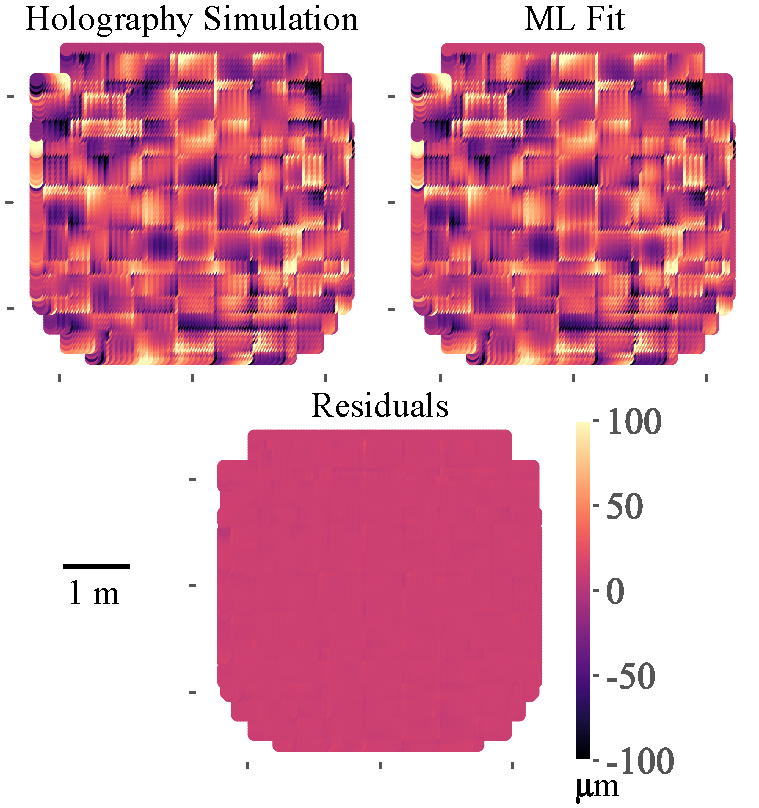
\includegraphics[width=.8\textwidth]{Figures/ap_length_corrected_single_pannel3.pdf}
    \caption{Results from simulation.  The top left panel shows the input simulation, which had 35 micrometer RMS HWFE.  The top right panel shows the predicted aperture phase given the ML determined estimates for the panel errors, and the bottom shows the residuals.}
    \label{fig:ap_resids}
\end{figure}
Here, we use a machine learning model built from the \verb|scikit-learn| python package~\cite{scikit}. To train this model, we generate a set of 1000 near-field beam simulations, each with a different realization of mirror setting errors.  Each beam simulation assumes an angular width of 200 arcmin., with 1 arcmin. spacing, for a total of 40,000 points in a 2d grid.  We then perform the holography analysis described above to yield a simulated data set comprised of aperture fields and the known input adjuster errors.  This suite of simulation is used to train a linear regression model.  The training took only minutes on a laptop, making the beam simulations the limiting computational step.  Once trained, this model will transform an input holography measurement into a set of estimated panel adjuster offsets.

Figure~\ref{fig:ap_resids} shows the results from a simulation.  The top left panel shows the input simulation, which had $35\,\mu$m RMS HWFE.  The top right panel shows the predicted aperture phase given the ML determined estimates for the panel adjuster positions, and the bottom shows the residuals.  An impressive feature of ML is that it achieved residuals below $3\,\mu$m for the combined HWFE for each of the 10 randomly chosen input simulations we tested.

\begin{figure}[t!]
    \centering
    \includegraphics[width=.9\textwidth]{Figures/m1m2_degeneracies.pdf}
    \caption{The left and middle columns show the surface errors on the Primary and Secondary mirrors after holography has been used to correct the mirror surfaces.  The right column shows the HWFE as a function of focal plane position.  The top row shows results for holography taken at a single position (see red dot).  The middle row shows results for binocular holography (combining measurements from two positions, see red dots).  The bottom row shows results for trinocular holography (combining measurements from three positions, see red dots).}
    \label{fig:m1m2_errs}
\end{figure}

One issue is that this fit is degenerate, in the sense that anti-correlated errors on the primary and secondary can cancel when measured from a single feed position.  To explore this, we plot the errors on the Primary and Secondary in Figure~\ref{fig:m1m2_errs}.  We also compute the half-wave front error on the aperture plane as a function of feed position across the large 2\,m focal plane used by SO to explore how the cancellation of this degeneracy varies with position.  The top row considers holography taken in the classical way with a single receiver position.  The middle row considers binocular holography, where two measurements taken at two positions are analyzed jointly to break degeneracies.  The bottom row further considers trinocular holography, where three measurements taken at three positions are analyzed jointly to further break degeneracies. 

These results show that standard single receiver holography leads to anti-correlated errors of $10\,\mu$m on each mirror, which cancel to less than $6\,\mu$m over most of a 2\,m focal plane.  The binocular results improve the mirror residuals to $6.5 \,\mu$m RMS, but still suffer from correlated errors that lead to HWFE marginally worse than for the single position holography.  These are below  $6.5\,\mu$m over much of the focal plane.  

The trinocular method improves the single mirror precision to $4\,\mu$m with suppressed degeneracies  which cancel  to better than $4\,\mu$m HWFE over all but the edges of the focal plane.   We have presented these results for a single realization of mirror errors, but we repeated the calculation 10 times and found the results to be robust.  Reducing the HWFE from panel setting to be below 5 $\mu$m requires trinocular holography.


%%%%%%%%%%%%%%%%%%%%%%%
\section{Measurement Practicalities and Robustness of Method}
\label{sec:meas_method}
Achieving results at this precision requires measurement hardware and methods with sufficient sensitivity and control of systematic effects, both of which are within reach.

The simulations were informed by the geography of the SO LAT site.  A 1\,km transmitter distance was chosen since the transmitter can be placed on the slope of Cerro Toco, a nearby mountain peak, at this distance and an elevation of $10^\circ$.  Given this choice, we can determine requirements on signal-to-noise and the knowledge of the location of the transmitter and receiver with respect to the telescope by varying these in our simulations.  Table~\ref{tab:tols} presents the results of this sensitivity analysis. 

We also tested the robustness of the ML method to differences between the (simulated) measured mirror surface and the training set.  We found that for measurements of mirror surfaces significantly worse than what was in the training set, the method gracefully degrades in a way that it fits out 90\,\% of the input surface.  For example, with a 100\,$\mu$m HWFE the difference between the input and fit results had an RMS of 10\,$\mu$m.  Repeating the measurement and alignment process a second time would reduce the alignment errors below our $5\,\mu$m target. 

\begin{table}[!b]
\centering

\begin{tabular}{|l|c|}
\hline
Minimum signal-to-noise & $80$\,dB\\
\hline
receiver position (arbitrary direction) & $2$\,mm \\
\hline
Tower source (radius) & $1.2$\,m \\
\hline
\end{tabular}
\caption{Allowed variation in signal-to-noise and positional knowledge needed to keep error contributions from these effects  below $2.5\,\mu$m HWFE.}
  \label{tab:tols}
\end{table}

The signal-to-noise requirement can be met with a source consisting of a Gunn Oscillator phase locked to an Oven Controlled Crystal Oscillator (OCXO).  Such a system can output hundreds of mW with a frequency stability of a few parts per billion.  This ensures the source remains reliably within a bandwidth of a few hundred Hertz, allowing for aggressive filtering of the received signals.  With this filtering, simple receivers based on harmonic mixers (noise temperatures of 100,000\,K) can in principle achieve signal-to-noises in excess of 130\,dB.  This enables broad illumination of the telescope to make the measurement immune to the source beam pattern and reduce the received signal power to below 1\,mW, a level that comfortably guarantees the detector response is within the linear regime and ensures more than sufficient signal-to-noise.

The position knowledge of the source and receiver can be measured with a combination of metrology and fitting in the analysis code.  The distance between the tower source and the telescope can be determined to better than 1\,m using a theodolite, which is a standard surveying tool.  The angular position of the source will be found with the central peak of the beam map.  Any residual errors in this angle are mitigated by the removal of a gradient in the phase on the aperture plane in the holography analysis.  The location of the receiver relative to the mirrors can be determined using a laser tracker to better than 1\,mm.  These positions can be verified by fixing one (e.g., the source distance) and then fitting the other (e.g., the receiver positions) using our simulation code.  In this way, we can determine and confirm these distances to ensure the phase corrections are correctly applied.  

The $x$ and $y$ positions of the panels are determined by centering the measured aperture fields in the coordinates used in the simulations.  We include this centering process in our results.  Therefore, this method is robust to alignment errors.

Three remaining issues, which can produce spurious phase variations in the aperture plane, must be considered: atmospheric fluctuations, the phase of the receiver feed, and the phase stability of the reference receiver.  The choice of 88 GHz should provide sufficient stability in the Chilean atmosphere at 17,000 feet.  This will be verified with repeated measurements.  The phase as a function of angle of the receiver feed will be measured in lab using the holography source and receiver.  It is straightforward to include this correction in the modeling code to remove its impact on these measurements.  Finally, the reference receiver must receive signals from the source without being affected by spurious reflections from the ground, and the cabling from it to the correlation receiver must be phase stable over the duration of the measurement.  The first concern can be addressed by feeding the reference receiver with a relatively high gain antenna, to exclude the ground, and mounting it off of the telescope to ensure its reflections aren't modulated.  The stability concern can be addressed with a scan strategy that revisits the beam center often to allow for the removal of drifts.  This approach also provides additional suppression of atmospheric phase effects.  

This approach and these considerations are similar to what was done for ALMA~\cite{alma_holog} and SPT~\cite{Carlstrom_2011}. The desired measurement precision is not significantly different from what was achieved in these previous measurements.  The SPT alignment residuals ($16\,\mu$m), were limited by the telescope stability rather than the measurement accuracy.  The measurement would take several hours to scan over $~2^\circ$, with arcminute resolution, once all hardware is fully set up.  A measurement at the desired precision is well within reach based on the measurement concept we have presented and these previous examples.

%%%%%%%%%%%%%%%%%%%%%%%%%

\section{Public Code}
\label{sec:code}
All code used for this paper is available on GitHub under the name \verb|HoloSim-ML|. The code includes two modules: beam simulation and holography analysis with mirror panel error fitting.  This beam simulation includes the mirror geometry and panel setting errors and computes the beam in both the near- and far-field regions.  The code can be adapted to produce the beam as a function of angle, as was used in this paper, or as a function of position in the focal plane.  The later may be more appropriate for a holography measurement using the method described in~\cite{fyst_holog}. The holography analysis code inverts complex beams either from simulations or holography data, corrects for near-field aberrations using ray tracing and returns the mirror surface errors.  We also include code that determines the near-field corrections following the analytic expressions presented in~\cite{alma_holog}.  The panel fitting code uses a machine learning algorithm  trained with beam simulations.  Notebooks are provided to show how to compute a beam simulation, how to analyze holography, and how to set up and run the panel fitting.  We invite users to adapt this code to any applications they see fit, but ask that publications using this code cite this paper and that code derived from this work remain public.

\section{Conclusion}
\label{sec:holosim_conclusion}
We have presented the simulation and analysis of holography data, including the application of machine learning techniques, to recover panel adjuster errors from a complex optical system comprised of two mirrors that create partially degenerate features seen in the phase on the aperture plane.  The power of machine learning is that it enables the efficient analysis of these data to separate the contributions of each mirror with high accuracy on small angular scales.  On larger scales, this method creates degenerate solutions which can be addressed with holography from multiple receiver positions.  The ML framework makes the analysis of these measurements from many receiver positions straightforward to analyze.  We presented an example of the SO dual reflector optical system and demonstrated that this approach can yield $<5\,\mu$m alignment errors, the requirement for SO science goals.

The approach demonstrated here comprises forward modeling of an optical system, sampling the system from multiple positions in the focal plane, and the application of ML to simultaneously determine many physical parameters which encode errors in the optical system.  While a standard fitting method could also work in this application, we found that after one month of fine-tuning, we were only able to fit out half of the RMS of this dual reflector system.  The ease of setting up and fitting with these ML tools was striking, while it also improved the quality of the fits for single mirror systems.  We anticipate that this approach can be applied to a variety of complex optical systems, including systems with multiple lenses, filters, absorbers, and other optical components.  For example, the SO~\cite{gali18} system includes re-imaging optics comprising three lenses, and filters.  An immediate future application is to apply these techniques, using holography, forward modeling, and ML to understand the optical properties and interactions within the system.  With proper parameterization of the imperfections and alignment errors, combined with sampling the focal plane at several positions, we anticipate that machine learning will prove to be an increasingly important tool in the characterization and performance optimization of complex optical systems. 

This software package developed for this work (\verb|Holosim-ML|~\cite{McMahonCosmologyLab}) is customizable to include arbitrary optics while remaining simple to script.  It is possible to substitute commercial simulation software within this ML framework if necessary.  However, we chose to write a self-contained code to create an open access package that is efficient and can be widely shared.
\chapter{The Atacama Cosmology Telescope: point source analysis of beams for DR6}
\label{ch:actbeams}

\section{\label{sec:act_intro}Introduction}
\setcounter{footnote}{0}

The Atacama Cosmology Telescope (ACT) is a 6\,m off-axis Gregorian telescope located at an altitude of 5190\,m in the Atacama Desert of northern Chile. It is designed for millimeter wavelength observations of the cosmic microwave background (CMB) at arcminute resolution.  The telescope and receiver are described in \cite{fowler_2007} and \cite{thornton_2016} respectively. 

This paper describes an alternative method for determining the optical response of the telescope based on stacking point source observations.  This data release includes temperature and polarization data collected by ACT between 2017 and 2021, covering roughly 18,000 square degrees of the sky~\cite{thornton_2016}.

Determining the optical response, or "beam", quantifies how the instrumental response is suppressed at small angular scales as a result of the finite resolving power of the optics.  For this reason, understanding the telescope beam and its uncertainty is critical for achieving the science goals of ACT.  Because the beam has to be de-convolved from the sky maps in order to perform cosmological analysis, incorrectly characterizing the beam directly biases any science by mimicking a spurious scale-dependent signal.  Therefor, in order to achieve the science goals set out by ACT, characterization of the instrument beam is crucial.  Besides the beam of the instrument, it is also important for a polarimetric instrument like ACT to quantify the amount of temperature-to-polarization leakage. We describe this type of leakage in terms of a so-called "leakage beam", quantifies the amount of leaked signal from Stokes I to Stokes Q or U at a given angular scale.

Previous work to characterize the ACT instrument beam have done so with planet maps (\cite{hasselfield_atacama_2013,louis_2017,naess_2014}).  Planets served as the best candidates for beam characterization of the telescope~\cite{Lungu_2022}.  Specifically, observations of Uranus achieve adequate signal-to-noise without exceeding the dynamic range of the instrument.  Here, we present a novel technique to characterize the instrument beam with map data, which we refer to as "stacking" of the point-sources in a map's catalog.  This work provides a detailed recipe for characterizing an instrument's beam using full map data, which we apply to the ACT DR6 maps.  This method provides a validation of the Uranus-derived beam both in temperature $T$ and in the $T\rightarrow E$ and $T\rightarrow B$ leakage.  Such a novel validation is necessary because the Uranus observations are separate observations made with a different strategy than the full maps, have different noise properties and were made using a different map-making technique.  The point-source stacking method, presented here, uses the same observations which we use for cosmology, thus providing a check to the beam and leakage inferred from Uranus observations.

\begin{figure*}[t]
\vspace{1em}
    \centering
    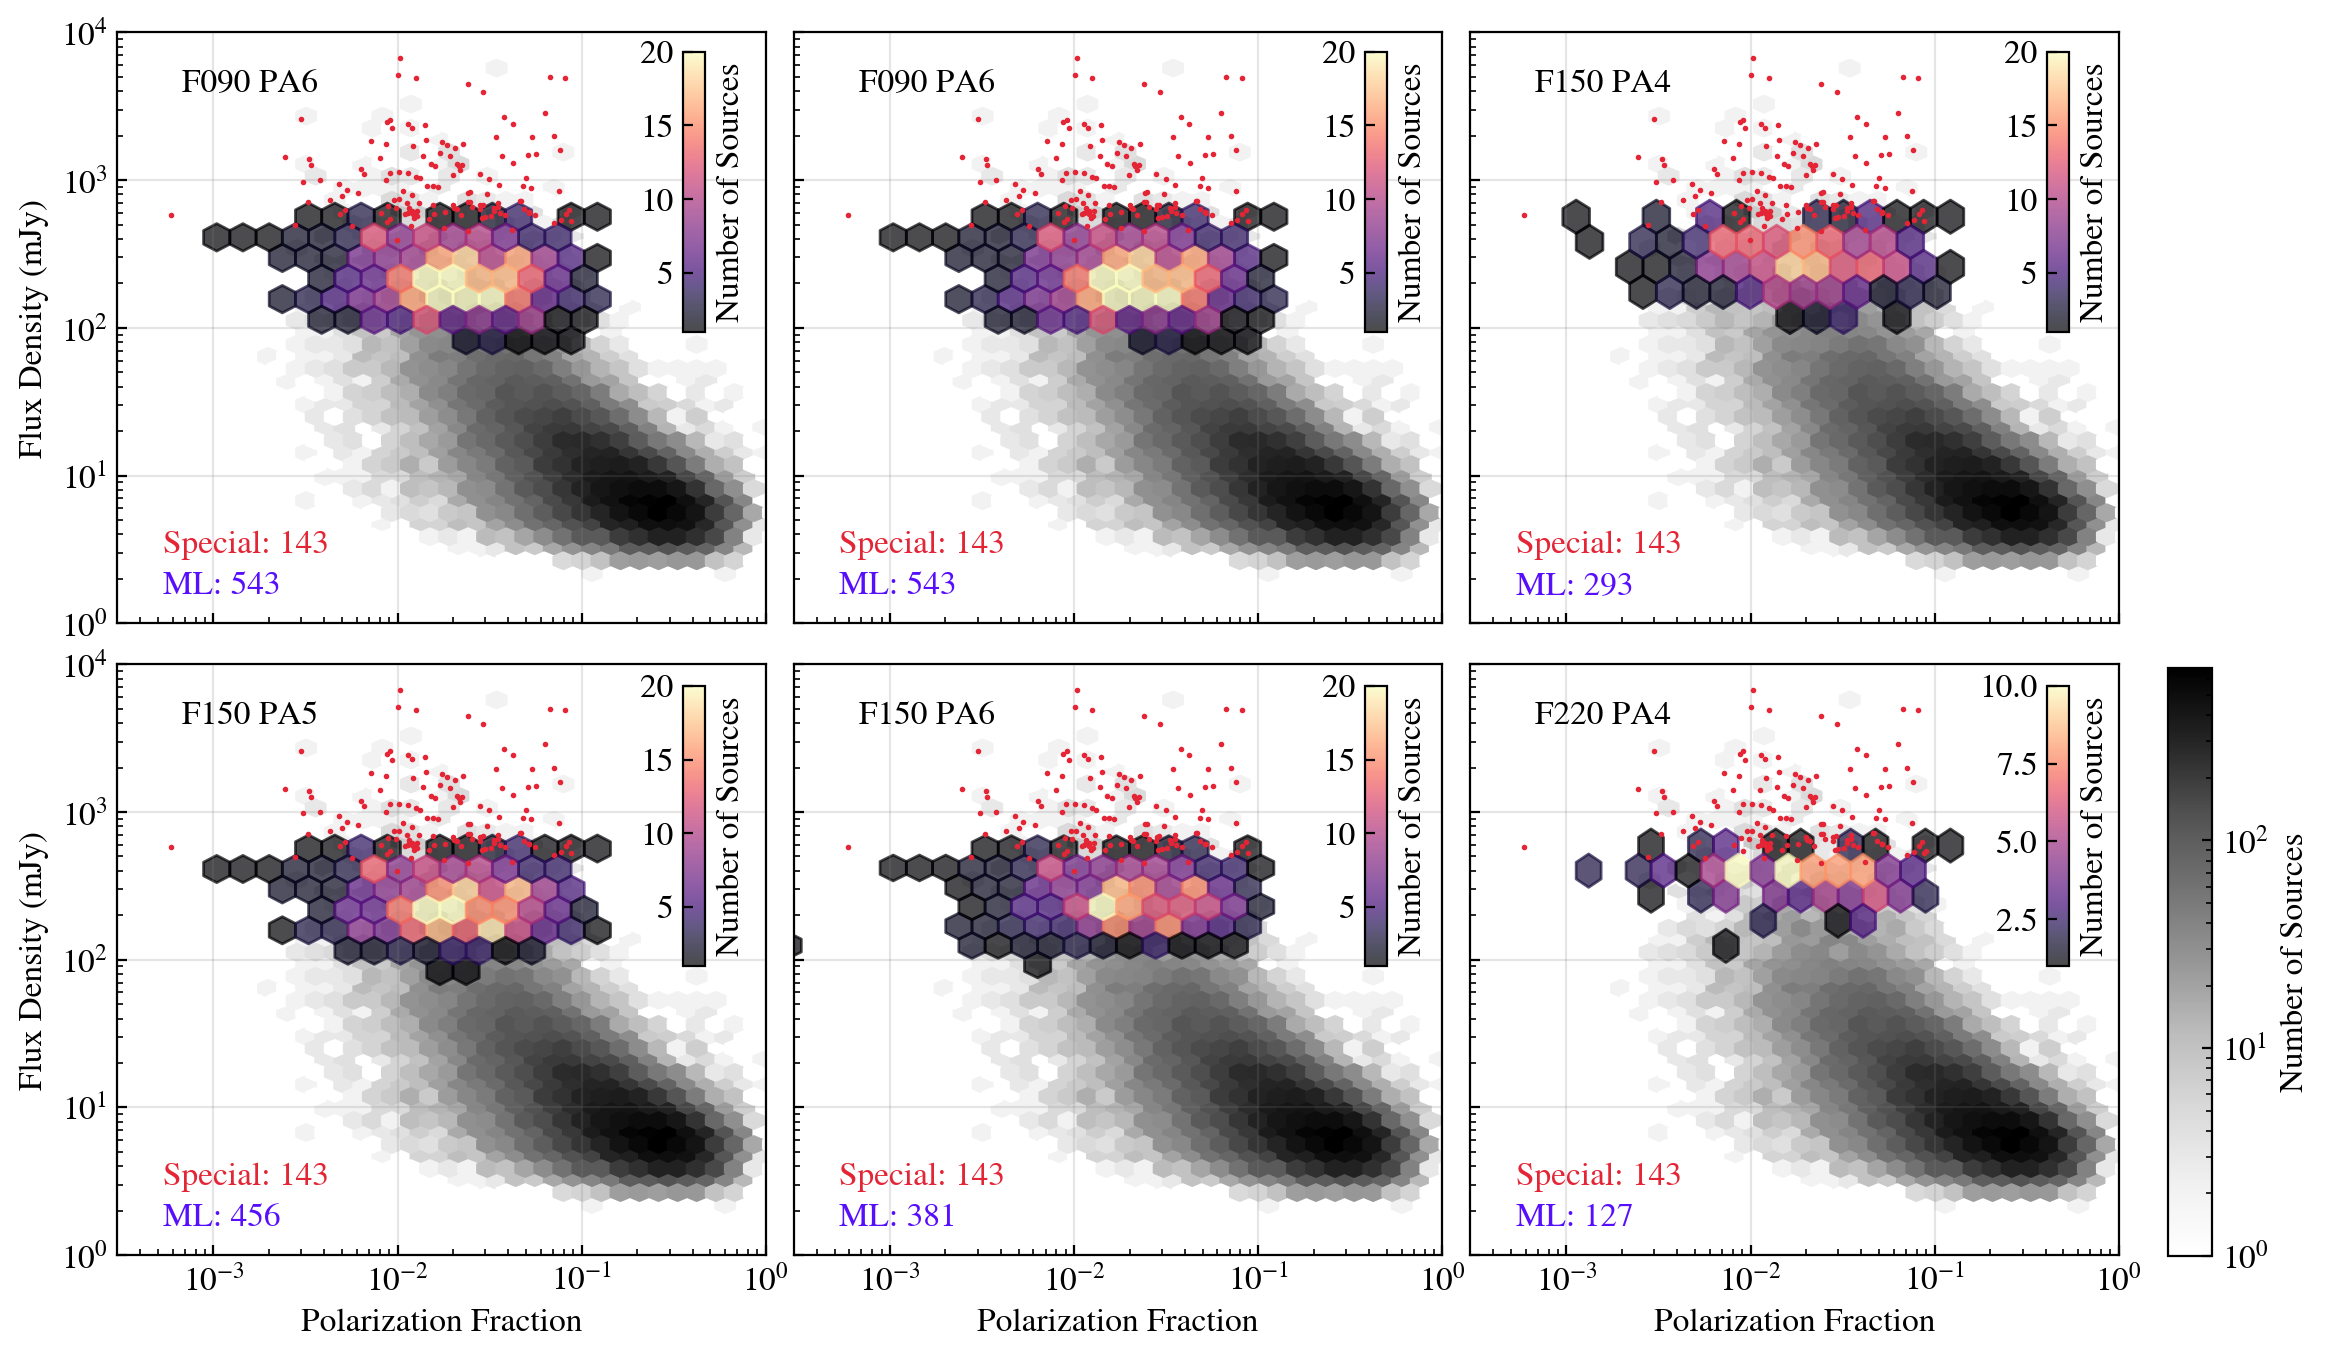
\includegraphics[width=\linewidth]{Figures/pt_src_dist.png}
    \caption{Distribution of the total number of point sources that were in the catalog (greys) and ultimately became part of the final beam analysis (colored) for all arrays combined, shown by observing seasons from 2017--19.  Point sources used in the stacking are separated into Special(red dots) and ML(gradient hexagonal bins) sources (the two types of sources are described in \S\ref{subsubsec:type_sel}).
    }
    \label{fig:ptsrc_select}
    \vspace{1em}
\end{figure*}

The paper is organized as follows.  In \S\ref{sec:observations} we describe the observations and catalog used to stack point sources and characterize the ACT beams.  In \S\ref{sec:stack} we explain the stacking process, starting from an input map and producing a stacked beam profile.  In \S\ref{sec:sim_pipe} we describe the steps of the map simulation pipeline, then going from simulated point-source maps to a model of the ACT beams and their covariance.  In \S\ref{sec:act_results} we present the results from the stacking method, including the stacked temperature to polarization leakage, and the temperature beam radial profiles.  Finally, in \S\ref{sec:act_disc} we discuss assumptions made in the analysis and future directions for ACT beam characterization.

\begin{figure*}[t]
    \centering
    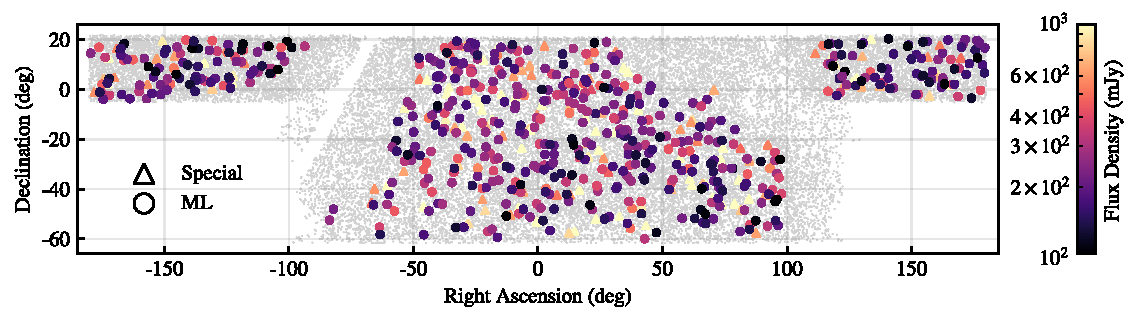
\includegraphics[width = \textwidth]{Figures/flux_map.pdf}
    \caption{Spatial distribution of all point sources in the catalog(grey) and the selected point sources used in stacking(colored).  The color bar shows the flux of the Special(ML) sources, which are plotted as triangles(circles).  The regions of the map with no used point sources indicate regions which are masked out prior to stacking.  The mask ensures that the stacked point sources are in the same regions of the sky used in cosmology science.}
    \label{fig:ptsrc_map}
\end{figure*}

\section{Observations}
\label{sec:observations}
The  data used in this work are part of the upcoming 6th data release (DR6) of ACT. DR6 consists of observation taken between 2017 and 2021 using three dichroic detector arrays, PA4, observing using broad frequency passbands roughly centered on  150 and 220\,GHz, and PA5 and PA6, both with passbands centered on 98 and 150\,GHz. The 3 types of frequency bands are referred to by f090, f150 and f220. On the sky, the observations fall in to the "Advanced Act" region as defined in \cite{aiola_2020}, which includes roughly 45\% of the full sky. The observations are taking during both day and night; in this work, we restrict ourselves to the nighttime data, as this subset of the data is the current focus of the cosmological analysis performed by the ACT collaboration. The DR6 data and analyses have not been made public yet at the time of writing.

The DR6 data are divided into 8 non-overlapping subsets and mapped into sky maps. In this work, we only use co-added versions of these 8 maps. We thus consider a single triplet of Stokes I, Q and U maps for each of the 6 combinations of PA4/5/6 and their two frequency bands. 

The maps are produced in the Plate-Carr\'{e}e cylindrical projection (CAR) using a maximum-likelihood (ML) technique that is described in \cite{aiola_2020}. There is one exception, which is relevant for this work: the brightest point sources are mapped with a specialized source mapmaker. This special treatment of bright point sources is needed because the ML mapmaker produces artifacts when mapping bright localized sources, see \cite{naess_2019} for a detailed explanation. In the DR6 maps, the specialized mapmaker is used for a pre-selected set of bright sources. We will refer to the bright sources that underwent this specialized treatment as "Special" sources, while we refer to the fainter sources that were mapped using the regular mapmaker as "ML" sources.

\section{Methods}
\label{sec:stack}
Here we walk through the stacking process from input map to beam profile.  

\subsection{Point-source Selection}
\label{subsec:ptsrc_sel}
Prior to stacking, we characterize each point source to determine whether they are suitable for stacking.  The number of point sources used for the point source analysis versus the total number of point sources in the catalog is shown in Figure~\ref{fig:ptsrc_select}.

\subsubsection{Select on Catalog}
\label{subsubsec:cat_sel}
For ease of interpretation, a sky mask is applied that is similar to those used by the various cosmological analysis. This mask removes regions with strong Galactic emission (based on the 353 GHz Planck data) and significantly noisy regions on the sky.  The point source catalog has been estimated from the DR6 maps using a matched filter approach. Through the use of the 3 ACT frequency bands, the catalog also includes an estimate of the type of each source (synchrotron, flat or dusty spectrum, as well as SZ clusters). The catalog will be described in forthcoming publications accompanying the DR6 release.

From the catalog, we obtain a list of RA's and DEC's of point-sources in the map.  However, it is not a given that each point-source from the catalog appears on our map, so we reject any coordinates which fall outside the boundary of the input map $\mathbf m$.  Additionally, we select only point synchrotron sources, such that we stack over individual point sources rather than galaxy clusters, rather than dusty galaxies or galaxy clusters.  The brightest sources are synchrotron sources; so these cuts do not significantly reduce signal-to-noise.  Rather, this cut simplifies the analysis by removing extended sources while we avoid stacking on sources with different spectral energy densities (and associated differences in optical response).

When stacking point sources, we restrain the point sources to a polarization fraction of below 10\% such that we are not dominated by highly polarized sources.  One would expect the polarization signal to intrinsically average out over the sources' random polarization angles.  However, this is not the case when a few of the brightest sources are strongly polarized and dominate the stack due to inverse-variance weighting (see Sec~\ref{subsubsec:beamqual_sel}), which up-weights sources with the highest signal-to-noise ratios.  Once the selection is complete, the geometry of the stamp is defined to be $40^{\prime}$($30^{\prime}$) wide at a $0.15^{\prime}(0.05^{\prime})$ resolution for the F090 and F150(F220) bands.  The region must be large enough such that the stamp will include side-lobes features, but resolved enough to make out the main beam profile.

\subsubsection{Select on Beam Quality}
\label{subsubsec:beamqual_sel}
With the list of point-source locations on our map from the catalog, we further decide which point-sources to use in the stamp based on a stamp's individual features.  For example, we don't want to include a stamp with two point-sources, or an off-center point-source, in the stack.  To characterize the quality of a point source, each point-source is re-projected to the same geometry (as specified in the last paragraph).  A point source $p_i$ is first peak-normalized.  If the location of its highest peak, $p_{i,1}$, is outside a radius of $0.5^{\prime}$, $p_i$ is assumed to be off-centered and is discarded.  

We next want to determine if the stamp has two point-sources or just one.  To do so, we find the second-highest amplitude in the stamp and assume this to be the second peak, $p_{i,2}$.  If the amplitude of $p_{i,2}$ is within 10\% of the average stamp value (outside the radius $r=\frac{2}{3}r_{\text{FWHM}}$), it is assumed to be dominant, and the point source $p_i$ is discarded.

Figure~\ref{fig:ptsrc_select} shows the number of point sources used in each band and PA from the catalog.  We note that the F090 map stacks included the greatest number of point sources, since the beams are larger and therefore take up a larger area of the stamp's area.  Because the F220 beams are much smaller in beam width, we constrain stamps in this band to a radius of $15^{\prime}$, while the F090 and F150 stamps are at a radius of $30^{\prime}$.

\subsubsection{Special vs. ML Sources}
\label{subsubsec:type_sel}
We subdivide the remaining point sources into two categories: Special and Max-Likelihood (ML) point sources.  When making the maps, as described in \S\ref{sec:observations}, point sources are treated with the two differing methods, and thus we want to consider the two groups individually when stacking to note any differences this treatment may have caused.  The final distribution of selected point sources is shown in Figure~\ref{fig:ptsrc_select}.

\begin{figure*}[t]
    \centering
    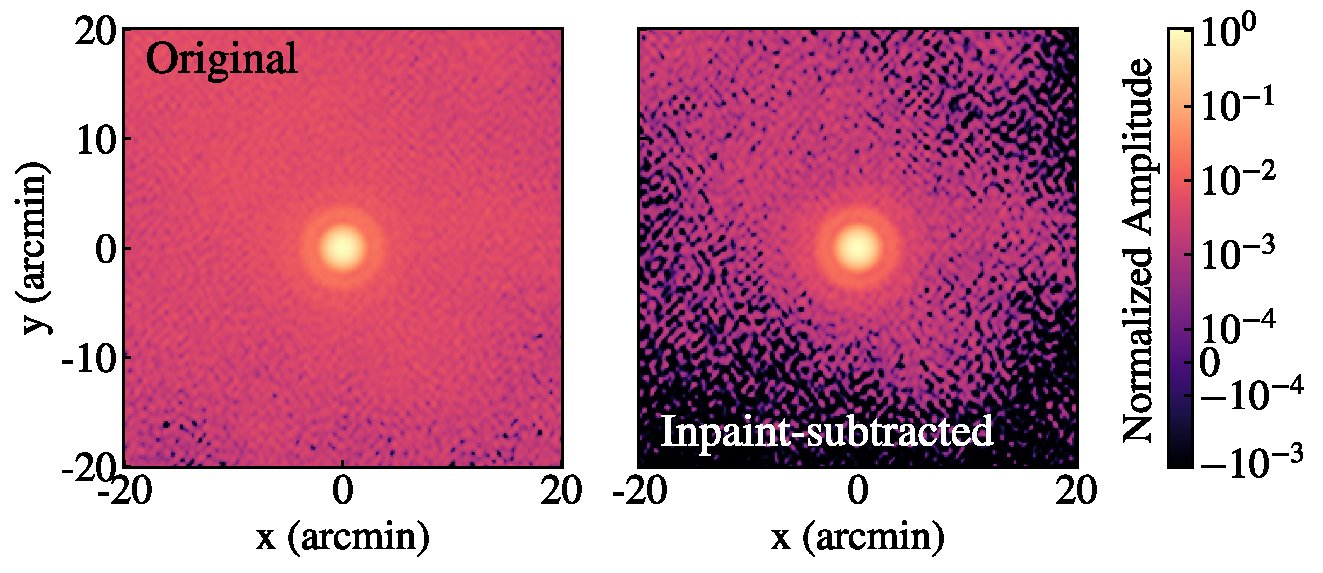
\includegraphics[height=.35\textwidth]{Figures/inpaint1.pdf}
    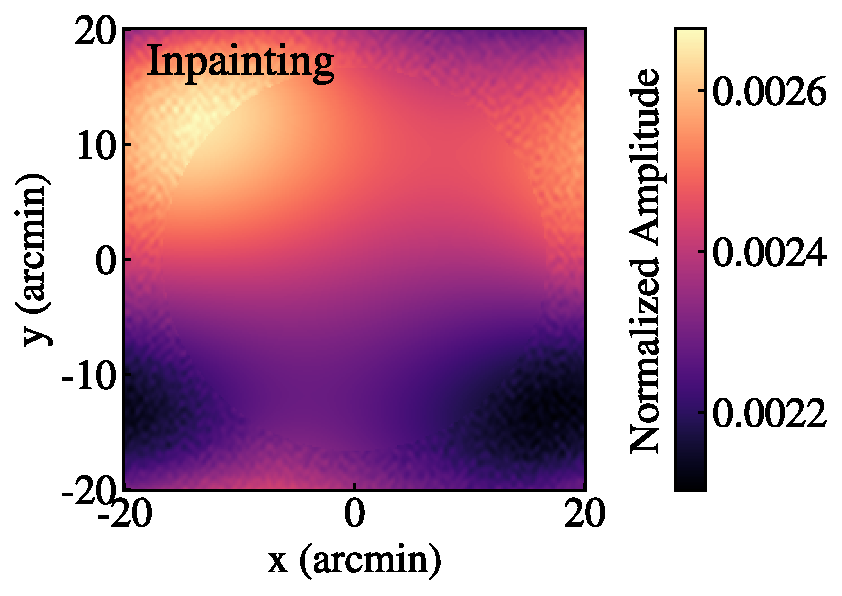
\includegraphics[height=.35\textwidth]{Figures/inpaint2.pdf}
    \caption{Inpainting-subtracted method as described in \S\ref{subsec:stacking} for F090 PA5.  Top row: Stacked beam without inpainting subtraction (left) and stacked beam including inpainting-subtracted method (right).  Bottom: Inpainting signal which is subtracted during the stacking procedure for F090 PA5 (note the linear scale colorbar).  This shows the large angular-scale signal which is removed from the stacked beam with the inpainting method.}
    \label{fig:example_maps}
    \vspace{1em}
\end{figure*}

\subsection{Stacking}
\label{subsec:stacking}
This section describes the stacking procedure with the selected sources.  Each stamp $s_i$ is re-projected to the same geometry prior to stacking.  Each stamp is cut from the map and re-projected to a tangent plane using a bi-cubic interpolation.  Re-projecting to a tangent plane ensures stacking multiple sources from different declinations are not stretched by different amounts (as a result of the CAR pixelization of the input map).  The bicubic interpolation introduces a small bias resembling a low-pass filter, which we investigate in \S\ref{sec:sim_pipe}.  We will show this bias is small enough to neglect.

Before stacking the reprojected stamps, we subtract an estimate of the large-scale correlated noise component of the stamp. The correlated noise, coming mainly from the CMB and atmosphere, is relatively bright compared to the point sources (at around the -20 dB level for even the brightest point sources), making it crucial to remove it prior to stacking.  If left in the stamps, the correlated noise is not averaged down enough during stacking as a result of the small number of high signal-to-noise sources in the stack. The resulting stacks show a large amount of noise variance that prohibits measurements of the non-central parts of the beam. We only perform the subtraction on the Stokes $I$ component of the stamps, the Stokes $Q$ and $U$ components have a relatively small amount of correlated noise, making the subtraction procedure unnecessary.

We refer to the subtraction method as ``inpaint-subtraction''. This procedure masks a region centered on the point source and fills this area with a prediction of large-scale correlated noise using only information from the outer area of the stamp. This inpainted region is then subtracted from the original stamp, resulting in a map of the point source with substantially reduced large scale correlated noise. The inpainting is done with a simplified version of the method described in~\cite{bucher_2012}. In short: the method uses the conjugate-gradient method~\cite{Shewchuk_1994} to solve for $s_l$ in:
\begin{equation}\label{eq:inpaint}
\left(S^{-1} + M^{-1} \right) s_l = M^{-1} s
\end{equation}
Here, $s$ denotes the input stamp and $S^{-1}$ denotes the covariance matrix of the correlated noise, modelled as a ``$1/f$'' spectrum in harmonic space: $1/ (1 + \ell / \ell_{\mathrm{knee}}^{-3})$ with $\ell_{\mathrm{knee}} = 2000$. This is a rough approximation of the actual covariance matrix of the correlated noise, but it works sufficiently well for our purpose. The $M^{-1}$ matrix is modelled in the pixel-domain, where it sets all pixels in the region around the point source to zero, and all pixels outside the region to a small, but nonzero value. The conjugate gradient method solves Equation~\ref{eq:inpaint} in roughly 10-20 steps, yielding $s_l$: a version of the stamp with an inpainted inner region that is smoothly connected to the outer region. The result of the inpainting-subtraction is shown in Figure~\ref{fig:example_maps}.

The above procedure will not bias the point source signal as long as the signal is zero in the unmasked outer region. In that case the information available for inpainting, i.e.\ the outer region, is independent of the point source and thus the inpainting-subtraction is unbiased by construction. However, due to the extended structure of the beam, the point source signal is not quite zero at the edges of the stamp where we define the outer region. As a result, the inpainting solution will not be perfectly uncorrelated to the point source signal, which means that once the inpainted stamp is subtracted, a small amount of the point source signal is also subtracted. This type of bias is similar to the one explained in the ACT DR4 beam paper~\cite{Lungu_2022}. To minimize the bias, we start the outer region at the radius at which the fiducial Uranus-derived beam becomes smaller than $10^{-4}$ compared to its peak value. Using the simulations in \S\ref{sec:sim_pipe} we validate that the remaining bias is small enough to ignore.
 
 The above inpainting procedure returns our point-source-free stamp, $s_{i,l}$.  We then subtract $s_{i,l}$ from our original stamp, $s_i$:
\begin{equation}
    s_i^{,} = s_i - s_{i,l}
\end{equation}
The final step is weighing each stamp and stacking them together.  We employ an inverse-variance weighting, where the weight is always calculated from the intensity $I_i$ stamp, and the same weight is applied the $Q_i$ and $U_i$ stamps.  The variance $\sigma^2$ is calculated between $r_{\text{in}}$ and $r_{\text{out}}$ of the stamp, where $r_{\text{in}}$ is defined as the radius where the Uranus-derived beam drops below $-35$\,dB (both $s_i^{,}$ and $s_p$ peak-normalized), and $r_{\text{out}}=\frac{4}{3}r_{\text{in}}$.  The weight of the stamp $w_i$ is then the inverse variance of $I$ within $r_{\text{in}}$ and $r_{\text{out}}$.  Once the above is calculated for all stamps in the set, the final stacked beam is calculated by:
\begin{equation}
    \bar{s} = \frac{\sum_i s_i w_i }{\sum_i w_i}
\end{equation}
Figure~\ref{fig:example_maps} shows an example output of the stacking, for PA5 F090.  Without inpaint-subtraction, the stamp appears saturated by large-scale structure (top left of Figure~\ref{fig:example_maps}).  The bottom panel shows the signal from inpainting which is subtracted from each point source stamp prior to stacking, leaving a less saturated stacked beam (top right).

\subsection{Bias From Stacking}
\label{subsec:bias}
To study this bias, a set of simulated observations are processed through the stacking process.  The full simulation pipeline is described in \S\ref{sec:sim_pipe}.

\subsection{Radial Profiles}
\label{subsec:profs}
Maps are binned into a symmetrized radial profile with bins of varying width, out to a radius of 20$^{\prime}$(15$^{\prime}$) for F090 and F150(F220), independently for each detector array, and F-band.  The bins are chosen to be logarithmic in radius.  We ultimately want to compare the stacked profiles to the Uranus-derived beams.  To do so, we first convert the Uranus-derived beams to a 2D stack matching the stamp geometry of the stacked beam.  We then radially bin the new Uranus-derived beam with the same bins used on the stacks.

Error of the radial profiles is obtained by simulating and stacking 100 maps with the simulation pipeline described in \S\ref{sec:stack} and \S\ref{sec:sim_pipe}.  The covariance matrix of these 100 simulated radial profiles estimates the error of our "true" stacked profiles at each binned radius.

\subsection{Beam Window Functions}
\label{subsec:window}
The window function $w_{\ell}$ quantifies the response of an instrument across angular scales, or multipoles $\ell$, which is encoded in the instrument's beam.  Because the CMB spectra is presented in spherical harmonic $\ell$-space, we similarly will compute the instrument's window function in $\ell$-space.  The window function is defined as
\begin{equation}
    w_\ell = B_\ell^2 \; ,
\end{equation}
where $b_\ell$ is a Legendre Polynomial transform of the instrument's beam (the full derivation of the Legendre transform is presented in~\cite{Lungu_2022}): 
\begin{equation}
B_{\ell} = \frac{2\pi}{\Omega}\int_{-1}^{1} B(\theta)P_{\ell}(\cos\theta)\; d(\cos\theta) \; .
\label{eq:legendre}
\end{equation}
Each $B_\ell$ is fixed at $\ell=1050$ for F090 and $\ell=1525$ for F150 and F220.  This $\ell$ range is the calibration value at which the ACT maps are calibrated to Planck, therefore we set the ratios of stacks to Uranus-derived beams to unity at this angular scale.

We quantify the leakage beams, or temperature power which has "leaked" into the Q and U polarization maps, by decomposing the Stokes $Q$ and $U$ stamps into $E$- and $B$-mode spherical harmonic coefficients~\cite{challinor_2000}:
\begin{equation}
\label{eq:pol_beam_coeffs}
b^{E}_{\ell m} \pm \mathrm{i} b^{B}_{\ell m} = - \int \mathrm{d}\Omega(\hat{n}) (Q \pm \mathrm{i} U)(\hat{n})\, {}_{\pm 2}Y^*_{\ell m}(\hat{n})
\end{equation}
Here ${}_{\pm 2}Y_{\ell m}$ are the spin-$\pm2$ spherical harmonic coefficients and the integral is taken over the whole sphere. $Q$ and $U$ represent the Stokes $Q$ and $U$ components of the stack rotated from the equator (where the stacks are centered) to the north pole of the standard spherical coordinate system. The rotation is done using the \texttt{pixell}~\footnote{\url{https://github.com/simonsobs/pixell}} library and takes into account the mixing of $Q$ and $U$ under rotations.  Similar to the reprojection mentioned in \S\ref{subsec:stacking} the rotation also makes use of bicubic interpolation. Again, through the simulations, we have validated that the resulting smoothing does not introduce a significant bias.

The $T\rightarrow E$ and $T\rightarrow B$ leakage beams are obtained from the $E$- and $B$-mode spherical harmonic coefficients in Equation~\ref{eq:pol_beam_coeffs}.  Here, we only present the symmetric part of the beam, i.e.\ the $m=0$ coefficients, though our analysis can also be used to study higher modes ($m=1,2$).  
The symmetric part of the leakage beam is modeled as:
\begin{equation}
B^{T\rightarrow E/B}_{\ell} = b^{E/B}_{\ell 0} \sqrt{\frac{4 \pi}{2 \ell + 1}}
\end{equation}
Where the $\sqrt{4 \pi / (2 \ell + 1)}$ factor converts from spherical harmonic coefficients to Legendre polynomial coefficients, which have the appropriate normalization. 

\section{Simulation Pipeline}
\label{sec:sim_pipe}

\begin{figure*}[t!]
    \centering
    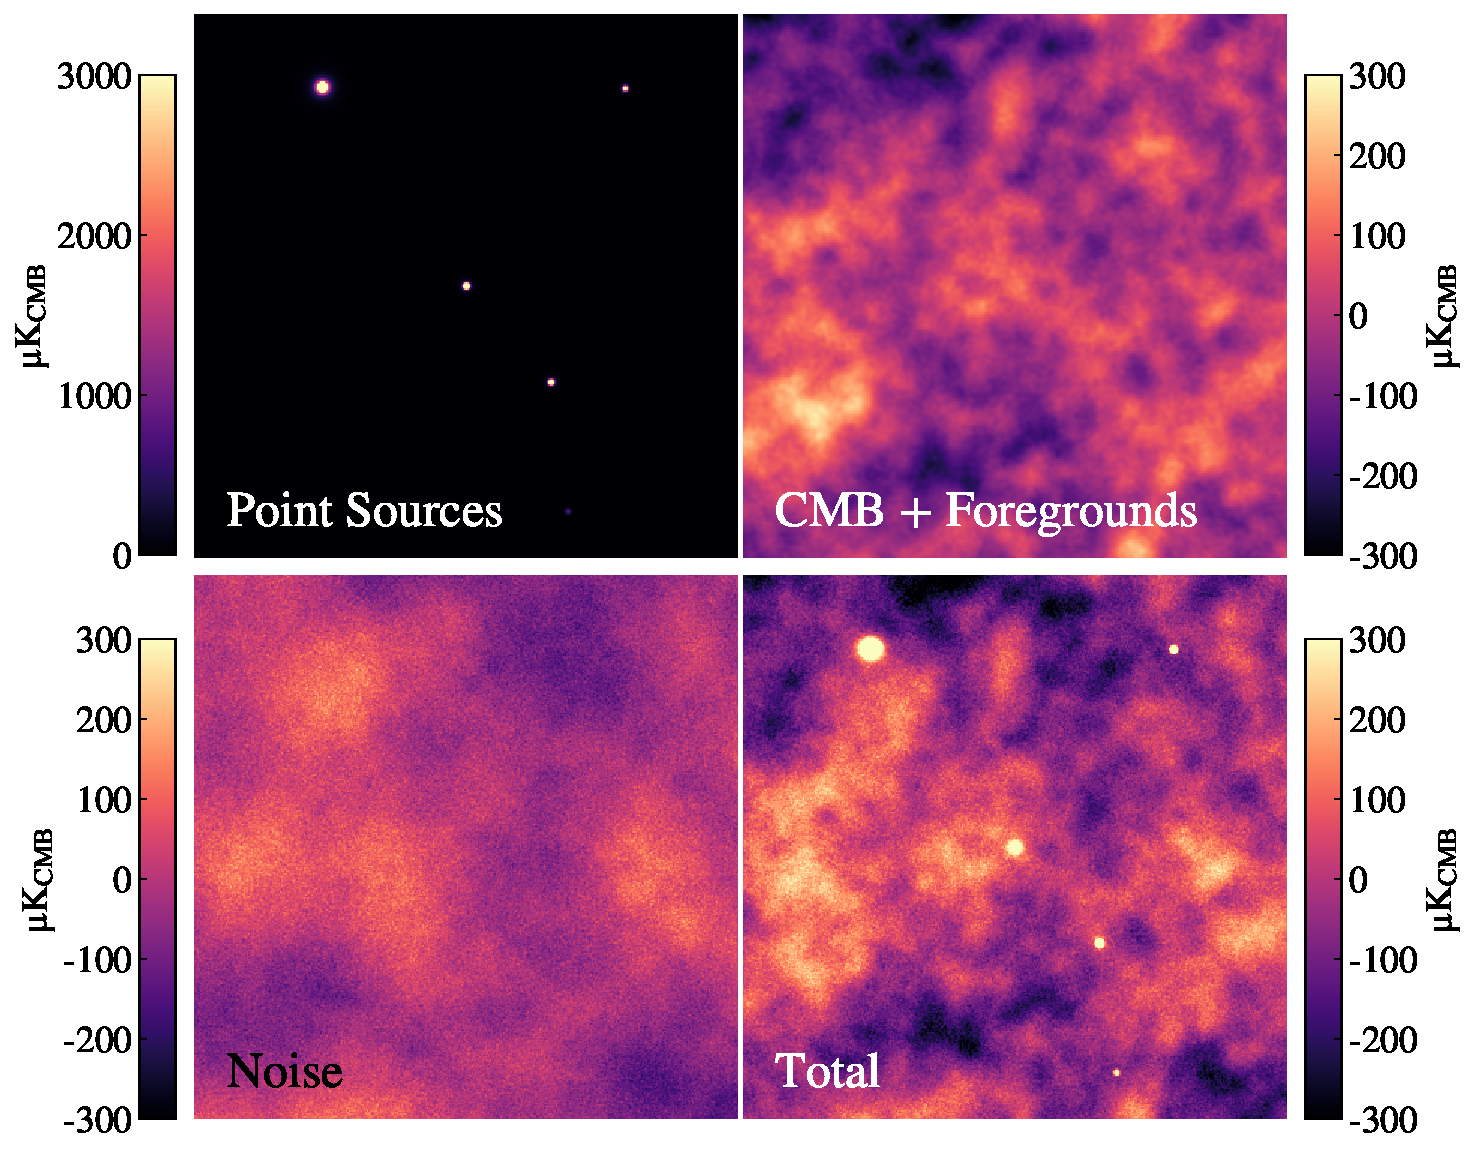
\includegraphics[width=\linewidth]{Figures/simmap.pdf}
    \caption{Example of a simulated map used to characterize the stacking bias.  This example is for PA5 in the F090, zoomed in to an area of $2\deg\times2\deg$.  Top left: Point-source map using the input catalog RA and DEC coordinates.  Top right:  Simulated CMB.  Bottom left:  Simulated noise~\cite{atkins}.  Bottom right: Final simulated map after combining the previous three components.  This process is done for each PA and F-band, and repeated 100 times to estimate radial profile errors.
    }
    \label{fig:sim_map}
\end{figure*}

We simulate a stacked profile to validate our stacking pipeline and to estimate statistical uncertainty on the radial profiles presented in \S\ref{sec:act_results}.  We first simulate a map by combining simulated point sources (referencing the catalog) along with a simulated CMB and foregrounds, and additionally adding simulated noise.  An example of a simulated map (box area of $\pm2\deg$ is shown in Figure~\ref{fig:sim_map}.  The four quadrants show the three main components of the simulated maps, followed by the total simulated map, where the prior three components are combined.  Here, we detail the construction of the simulations.

\subsection{Point Source Map Simulation}
\label{subsec:sim_ptsrc}
A point source map is simulated using the input catalog, and point source selection described in \S\ref{subsubsec:cat_sel}.  The Uranus-derived beam defines the shape of the point sources in the simulated map.  Fluxes of each point source are obtained from the catalog and converted to the units of the data maps ($\mu \text{K}_\text{CMB}$) using the fiducial beam solid angle and center frequency of the passbands.

The fiducial beam profile, fluxes and coordinates are then given to the \verb|pixell.sim_objects| function that outputs a simulated point source map with matching point sources and map shape as the catalog and DR6 map. We choose to apply to the simulated map a pixel window function that matches that of the data maps for ease of comparison.

\subsection{CMB Simulation}
\label{subsec:sim_cmb}
The second component of the simulation is diffuse sky signal comprised of the CMB and (extra-)Galactic foregrounds.  This signal is critical in the simulation because the CMB is a significant source of noise in our stacked profiles at intermediate angular scales.  To accurately estimate the uncertainty and bias introduced by the inpaint-subtraction method described in \S\ref{subsec:stacking}, we must include the CMB in our simulations.

We use the DR4 $C_\ell^{TT}$ power spectra to draw Gaussian realizations of the diffuse sky signal. An example of this simulated signal is shown in the top right of Figure~\ref{fig:sim_map}.  This simulation also contains foregrounds, which are an important contribution at high multipoles.

\begin{figure*}[t]
    \centering
    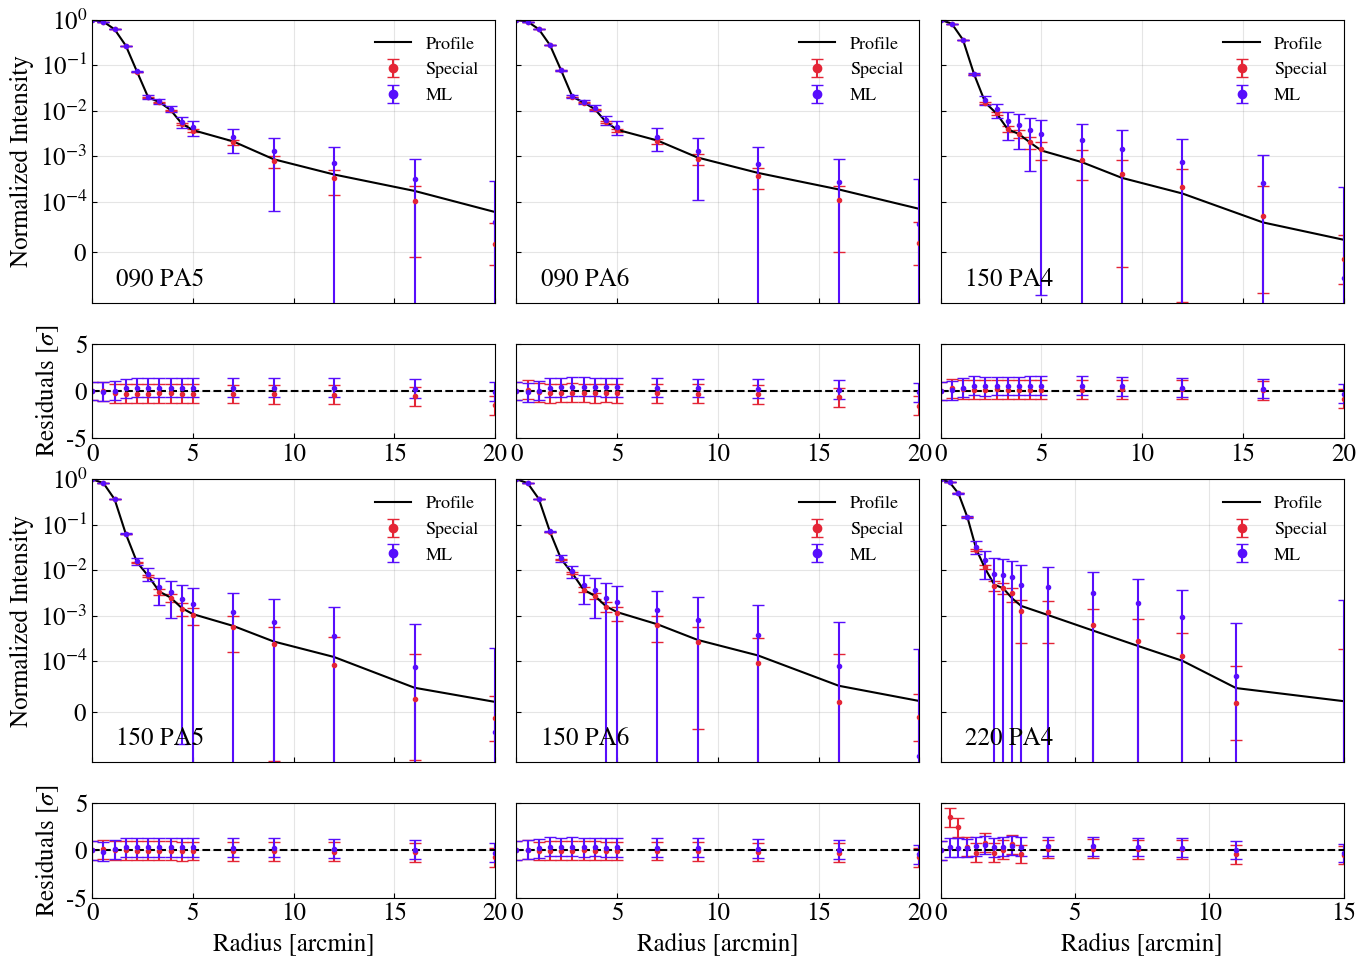
\includegraphics[width=\textwidth]{Figures/profiles_sims.png}
    \caption{Mean simulated radial profile at each F-band and PA, averaged over 100 simulations.  Mean simulated profiles are shown for Special(red) and ML(blue) sources, with error bars calculated from the covariant matrix of the 100 profiles.  Each profile is then compared to the corresponding Uranus-derived beam(black) in the bottom panel of each plot.  This shows the bias from the stacking procedure is minimal and can be neglected in the subsequent analysis.}
    \label{fig:simprofs}
\end{figure*}

\subsection{Noise Simulation}
\label{subsec:sim_noise}
The third component to complete our simulated maps is noise.  The estimation of map noise is twofold: 1) a realization of the ACT map-based noise simulations at large angular scales ($\ell<5000$) and 2) a white-noise realization drawn from the per-pixel variance maps that accompany the DR6 maps.

The ACT map-based noise simulations will be fully described in an upcoming paper accompanying the DR6 release. Noise simulation maps include atmosphere, ACT scan strategy, and a more detailed approach to model correlated instrument noise.  An individual noise simulation is used for each individual simulated map.

As the map-based simulations at the time of this analysis only describe the noise on large angular scales ($\ell<5000$), we manually fill in the noise on small angular scales.  We then splice together two noise simulations in $\ell$-space, such that the white noise term occupies the lower $\ell$-space and map-based noise dominates the high $\ell$-space.  An example patch of the noise map is shown in the bottom left of Figure~\ref{fig:sim_map}.

Figure~\ref{fig:simprofs} shows the mean simulated profile (over 100 simulations) at each PA and F-band compared to the Uranus-derived beam, plotted in black.  From this averaged simulated beam, we determine the stacking procedure to have negligible bias on the resulting beam profile.

\section{Results}
\label{sec:act_results}
Here, we detail the resulting temperature and temperature-to-polarization leakage beams acquired from the stacking method described above. 

\begin{figure*}[t]
    \centering
    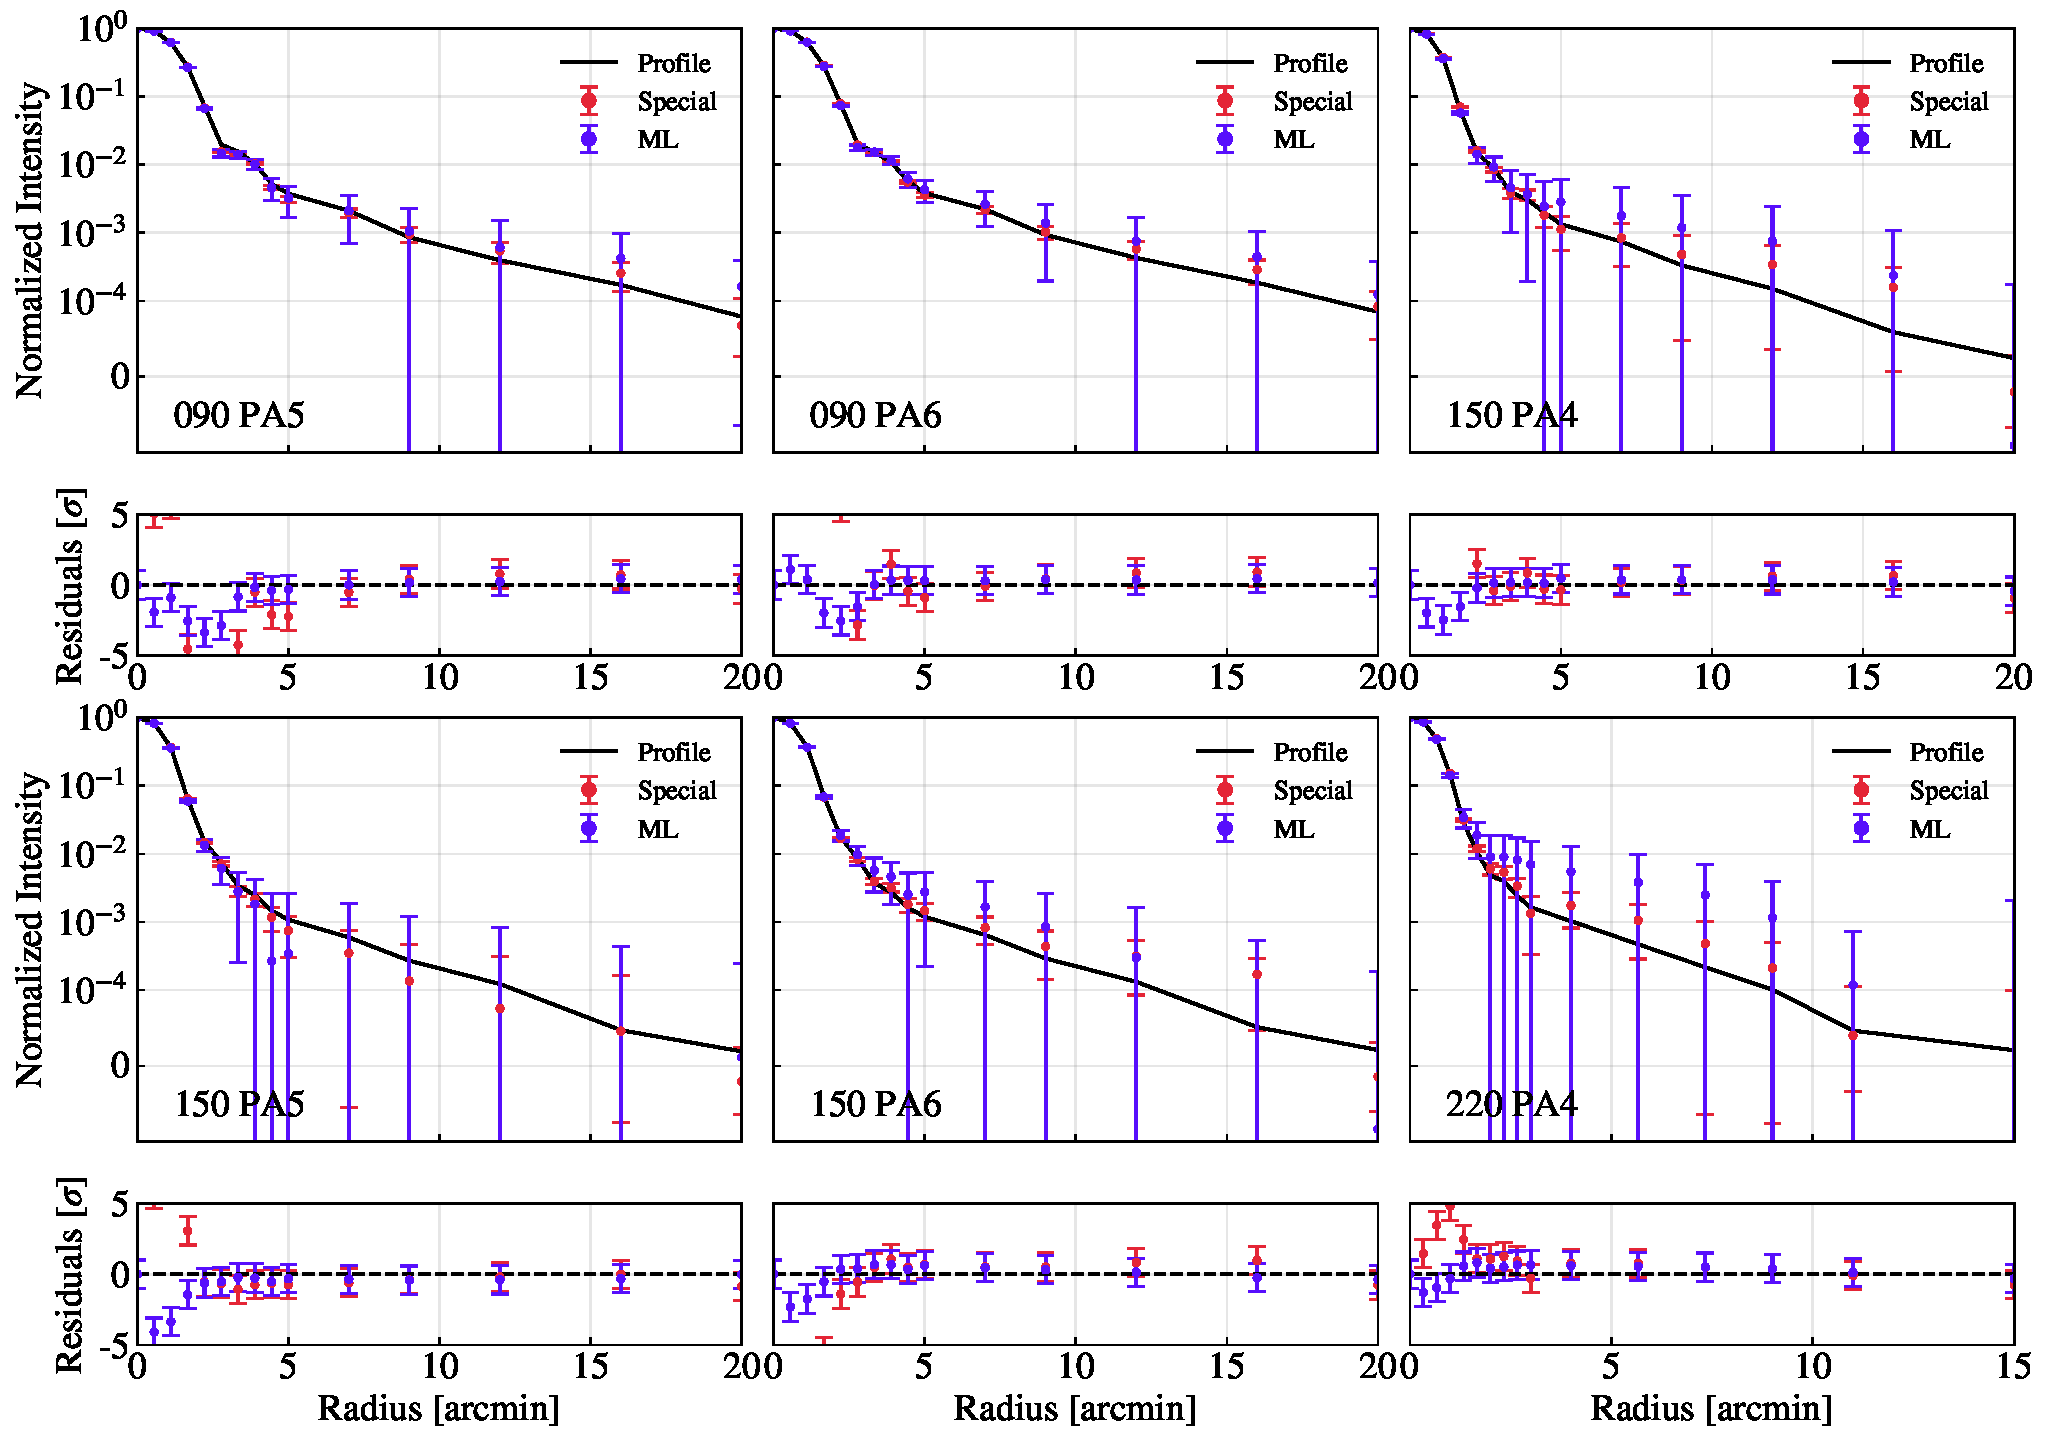
\includegraphics[width=\textwidth]{Figures/profiles_noP_15.pdf}
    \caption{Stacked radial profile at each F-band and PA.  Profiles are shown for Special(red) and ML(blue) sources, with error bars calculated from the covariant matrix of 100 simulated stacked beams.  Each profile is then compared to the corresponding Uranus-derived beam(black) in the bottom panel of each plot.
    }
    \label{fig:profiles}
\end{figure*}

\subsection{Main Beam}
\label{subsec:mainbeam}
This section presents the temperature profiles from stacks and compares them to the existing Uranus-derived beams from Uranus. 

\subsubsection{Profiles}
\label{subsubsec:profiles}
The stacked profiles are shown in Figure~\ref{fig:profiles}.  Each profile shows the Uranus Uranus-derived beam in black, with individual arrays plotted separately.  The bottom panel shows the difference between each array's profile to the planet.

\subsubsection{Spatial Variation}
\label{subsubsec:null_mainbeam}
To study the spatial variation of point sources, we conducted a "null test" where we stacked four categories of point sources: high and low, RA and DEC.  We separate the catalog in half by considering the median RA and DEC, such that the four categories are $\text{RA}_{\text{low}}$, $\text{RA}_{\text{high}}$, $\text{DEC}_{\text{low}}$ and $\text{DEC}_{\text{low}}$ (separated by their median values). 
 Figure~\ref{fig:bells} shows the resulting window functions $B_{\ell}$ for each F-band and PA.  The red line in each sub-plot show the full map's $B_{\ell}$ for comparison.

From this test, we find the Special sources have spatial dependence where the $\text{DEC}_{\text{low(high)}}$ and $\text{RA}_{\text{high(low)}}$ match in window function, but differ from their opposite.  Specifically, the Special sources consistently show larger power at high $\ell$'s in the $\text{DEC}_{\text{low}}$ and $\text{RA}_{\text{high}}$ than the Uranus-derived profiles, indicating a tighter beam in these regions of the sky.  This effect is most prominent in the F090 PA5/6 and F150 PA4 profiles.  The ML sources, however, do not show this effect, as we note less variation between the profiles when separated by regions of the sky.

\begin{figure*}
    \centering
    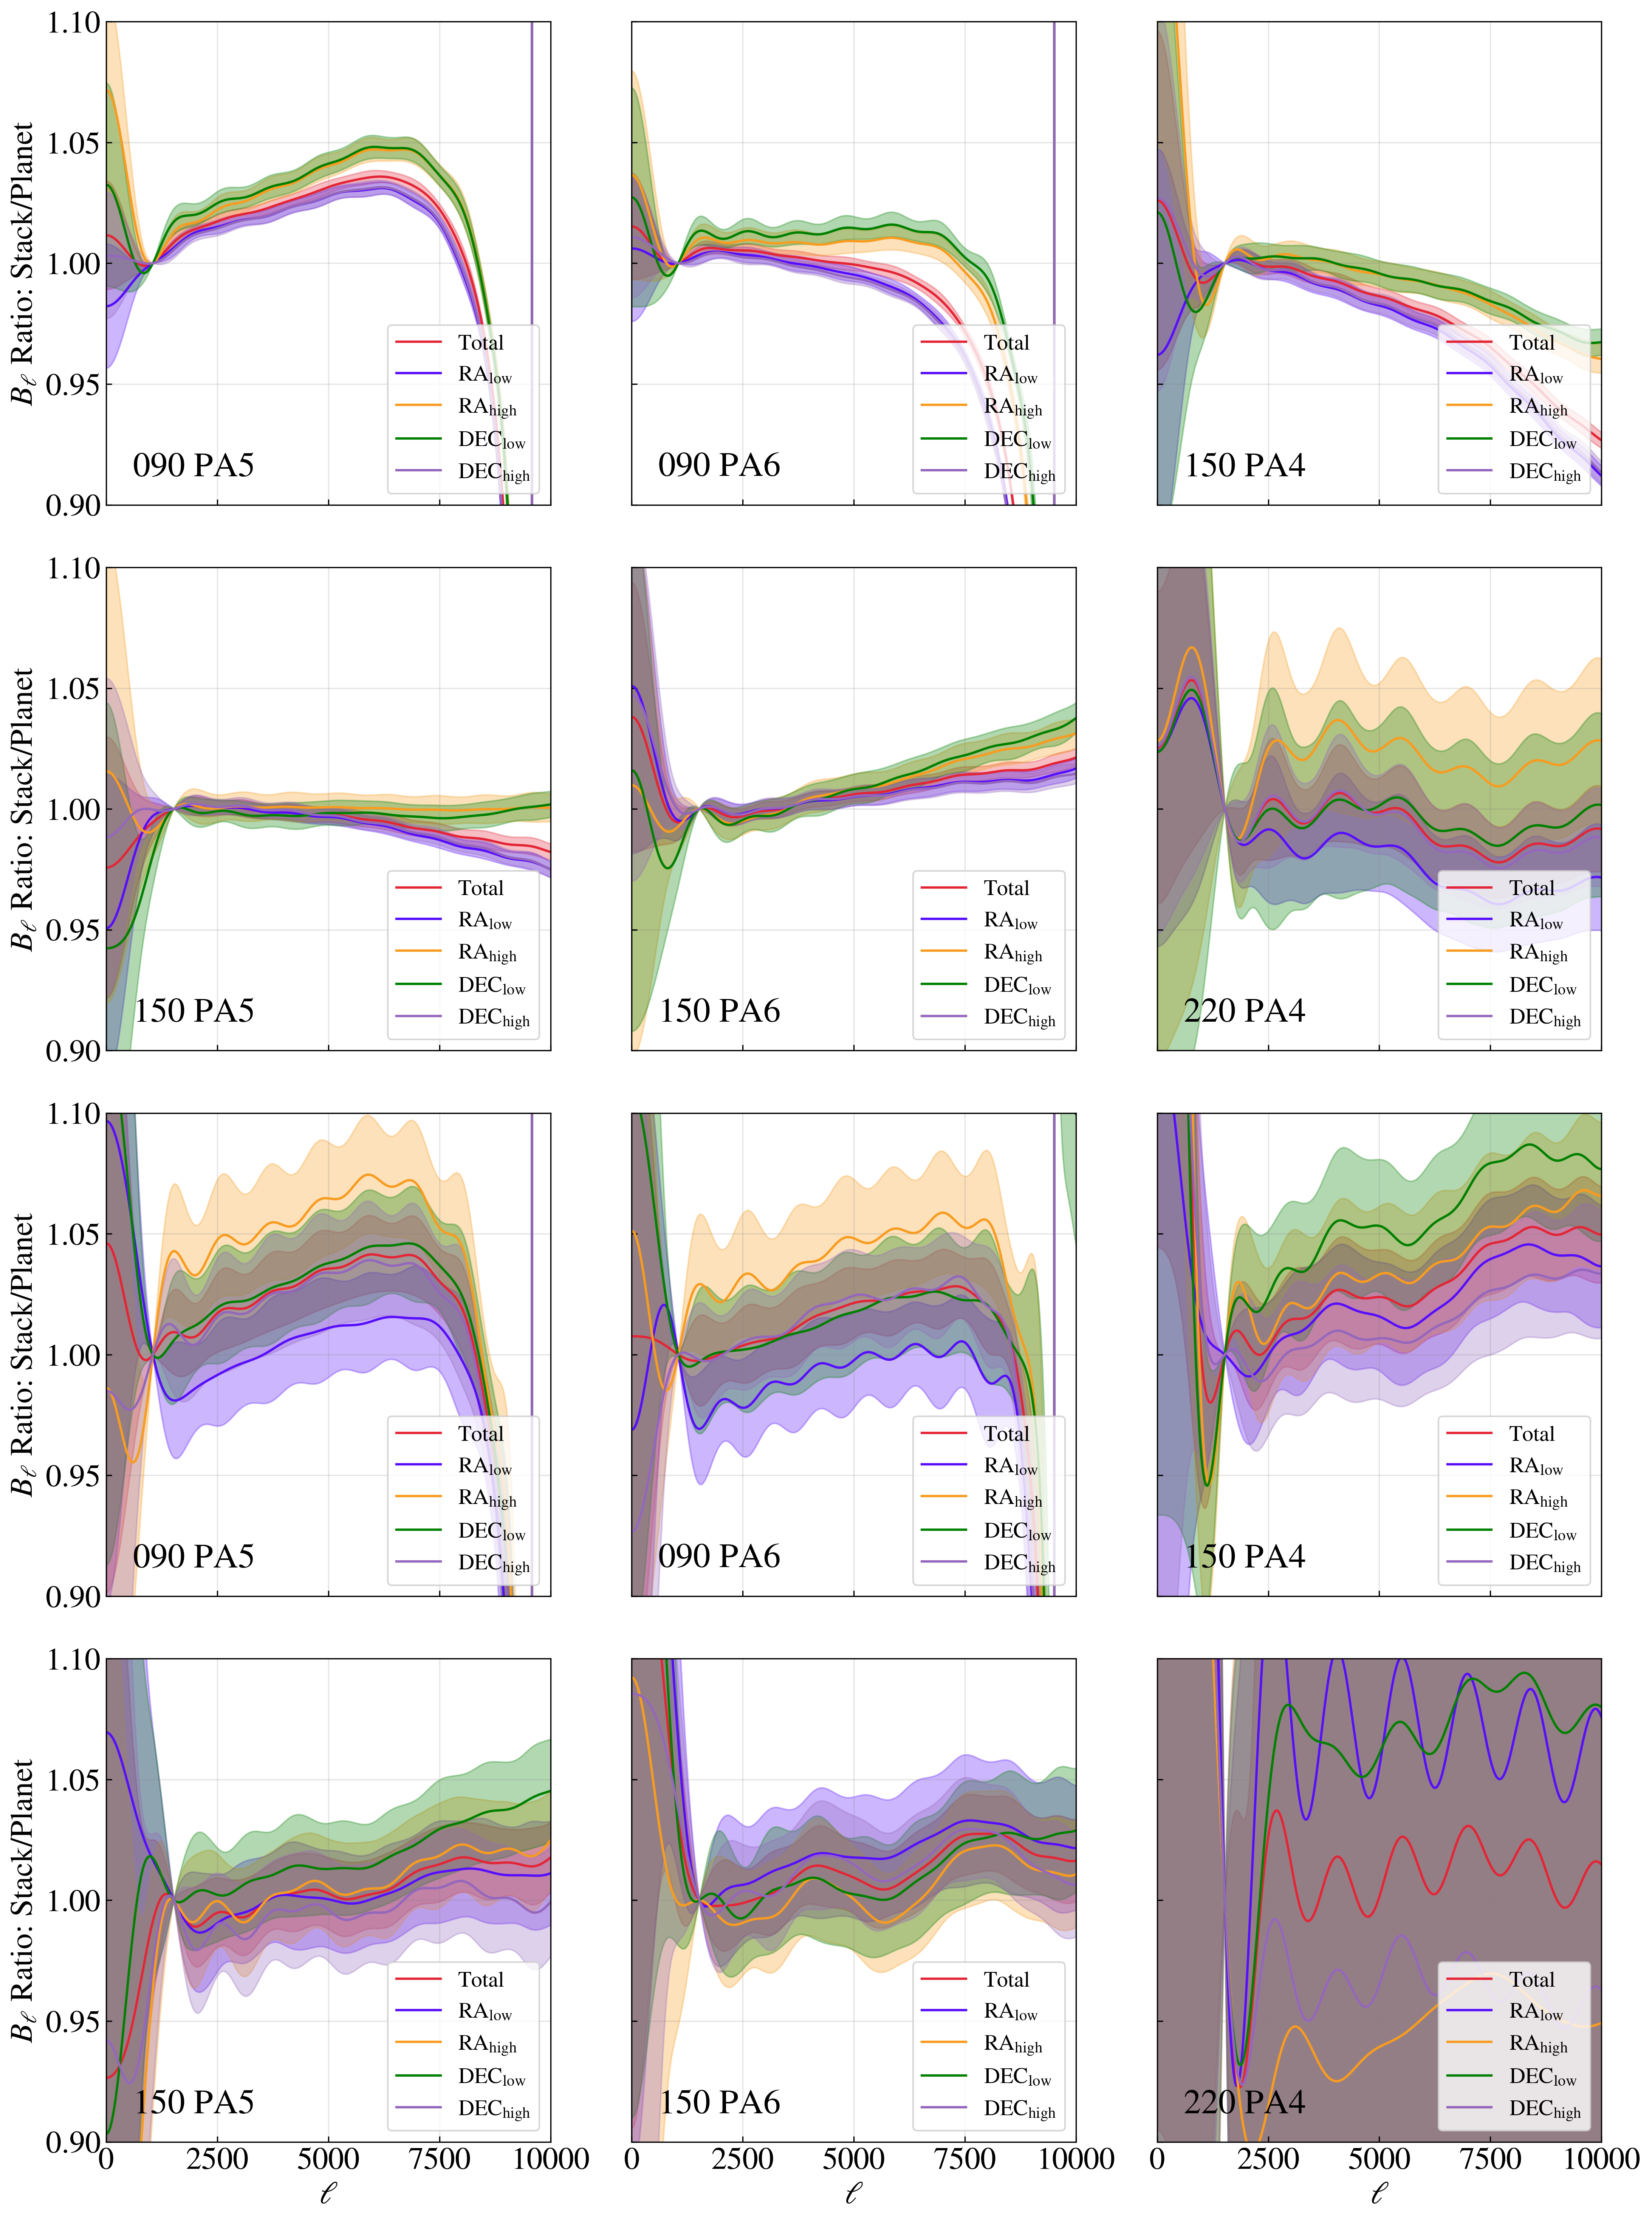
\includegraphics[width=.9\textwidth]{Figures/Bells_ratio_planet.pdf}
    \caption{Window function of stacked point sources, separated by high and low RA and DEC, which we consider as a null test.  The top two rows are Special sources, and the bottom two rows are the ML sources.  Each ratio is normalized to $B_\ell =1$ at $\ell=YYY$.  The full map stacked is plotted in red.  This test presents a spatial variance of the stacks.}
    \label{fig:bells}
\end{figure*}

\subsection{Temperature to Polarization Leakage Beam}
\label{subsec:polbeam}
\begin{figure*}[t]
    \centering
    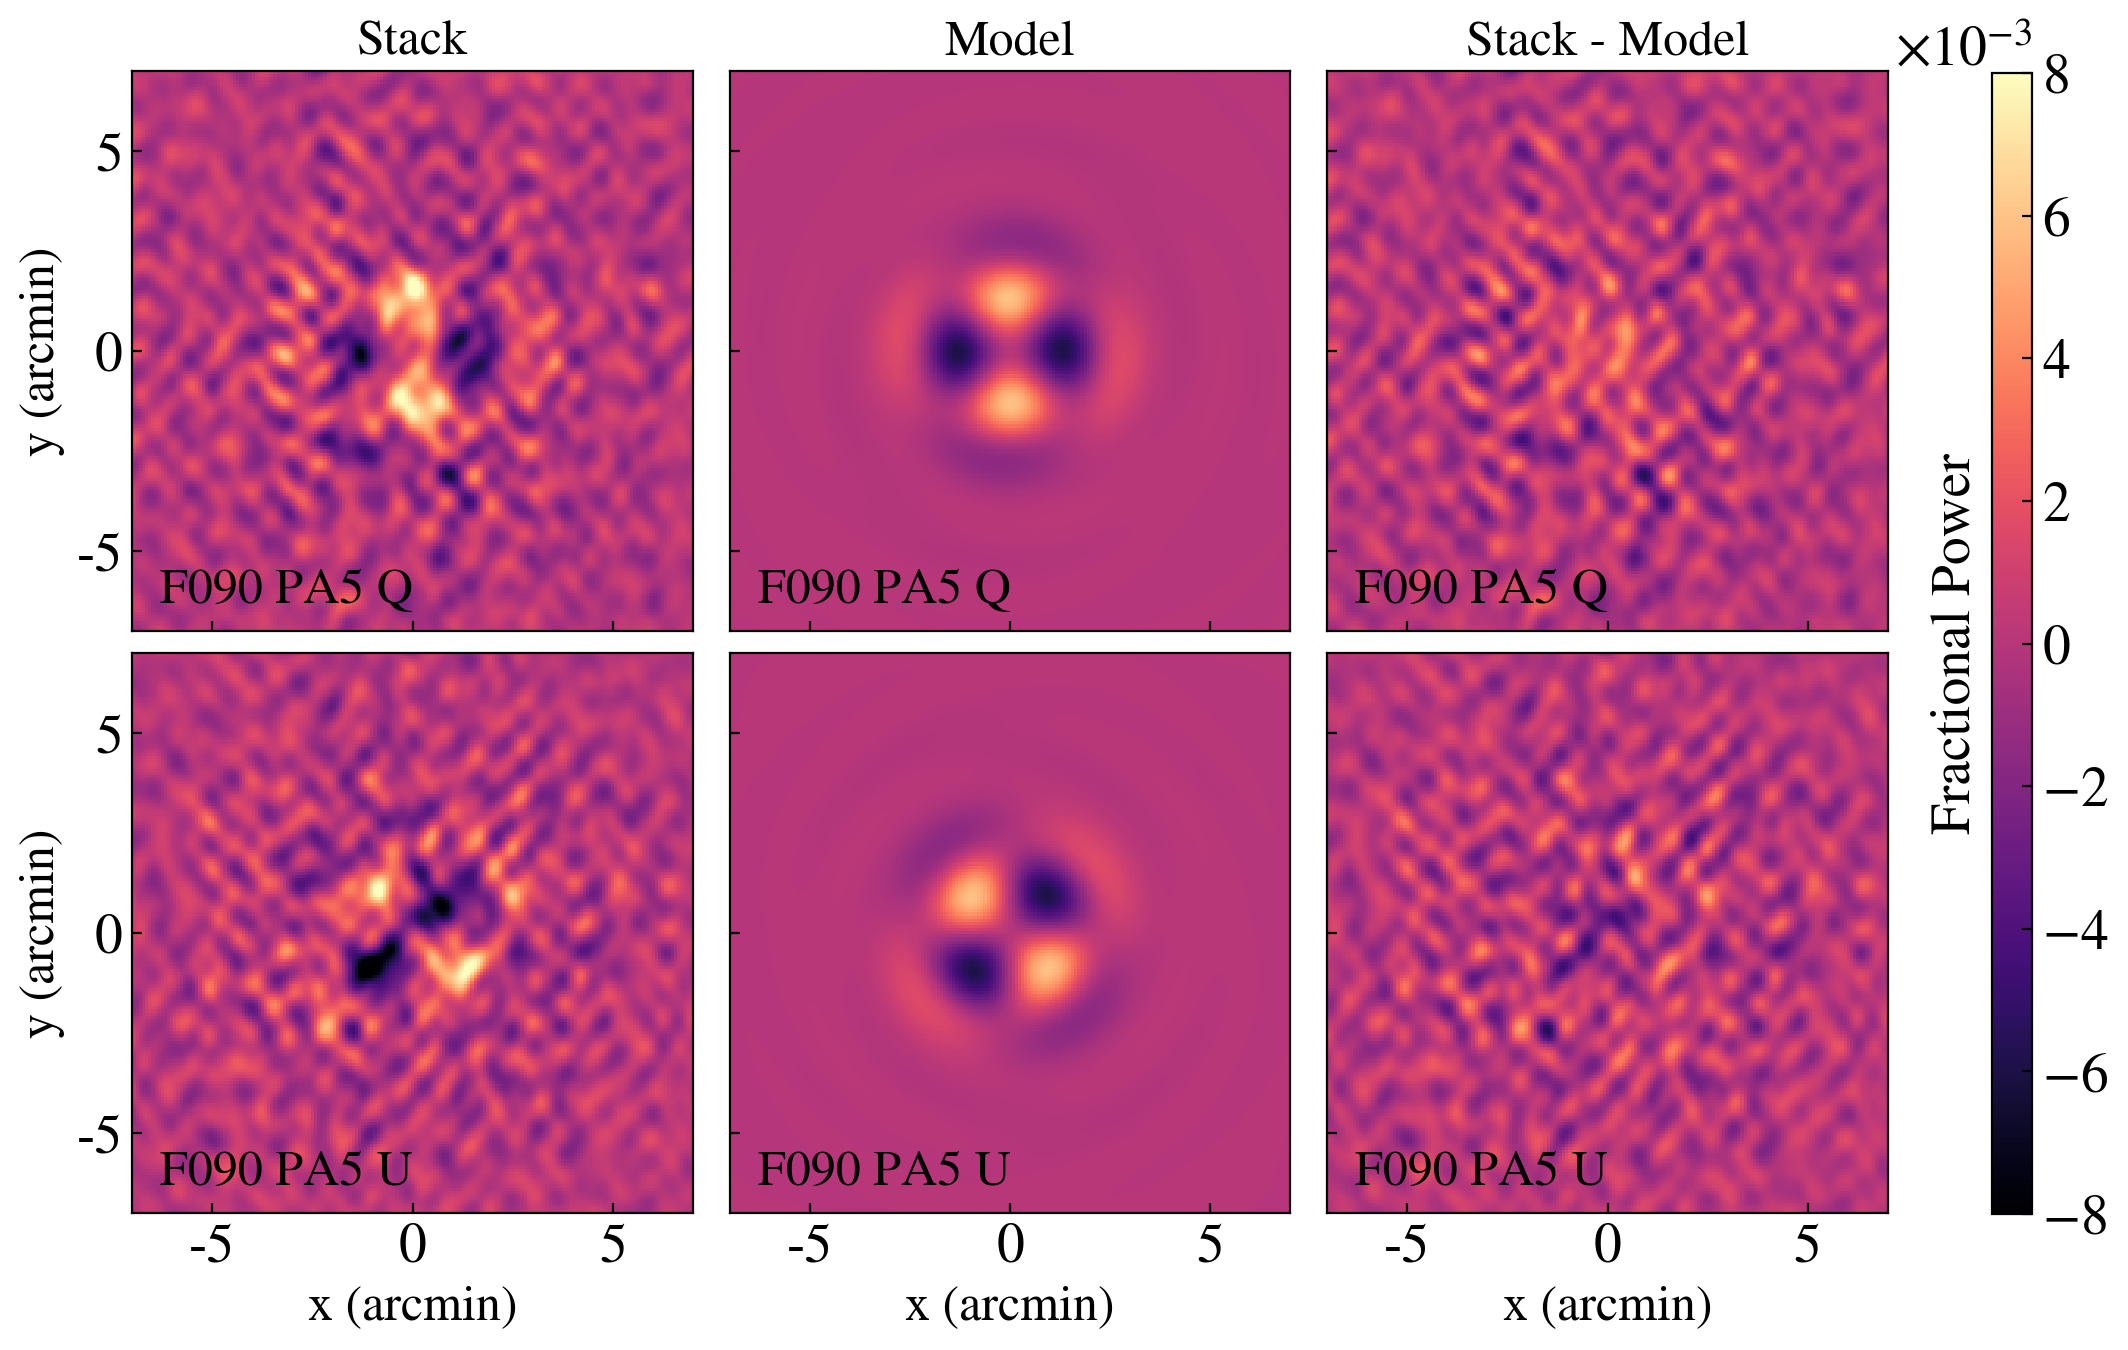
\includegraphics[width = \textwidth]{Figures/polbeams.png}
    \caption{Polarization leakage from stacked F150 PA4 beam, for the ML sources.  Top row: Q polarized beam.  Bottom row: U polarized beam. 
    Left column: stacked map, Middle column: modeled polarization leakage, Right column: difference between stacked and modeled beams.}
    \label{fig:polmodel}
\end{figure*}
Here, we present the polarized beams of the stacked point sources to determine polarization leakage in the instrument.  The leakage is relatively small compared to the magnitude of the temperature beam, however the sensitivity of ACT DR6 data is such that this leakage needs to be accounted for in the analysis.  Previously, observations of Uranus were used to build an $\ell$-space T-to-P leakage function for a given frequency and array in the instrument.  Here, we test this method by comparing the leakage to our new method of stacking.

\begin{figure*}[t]
    \centering
    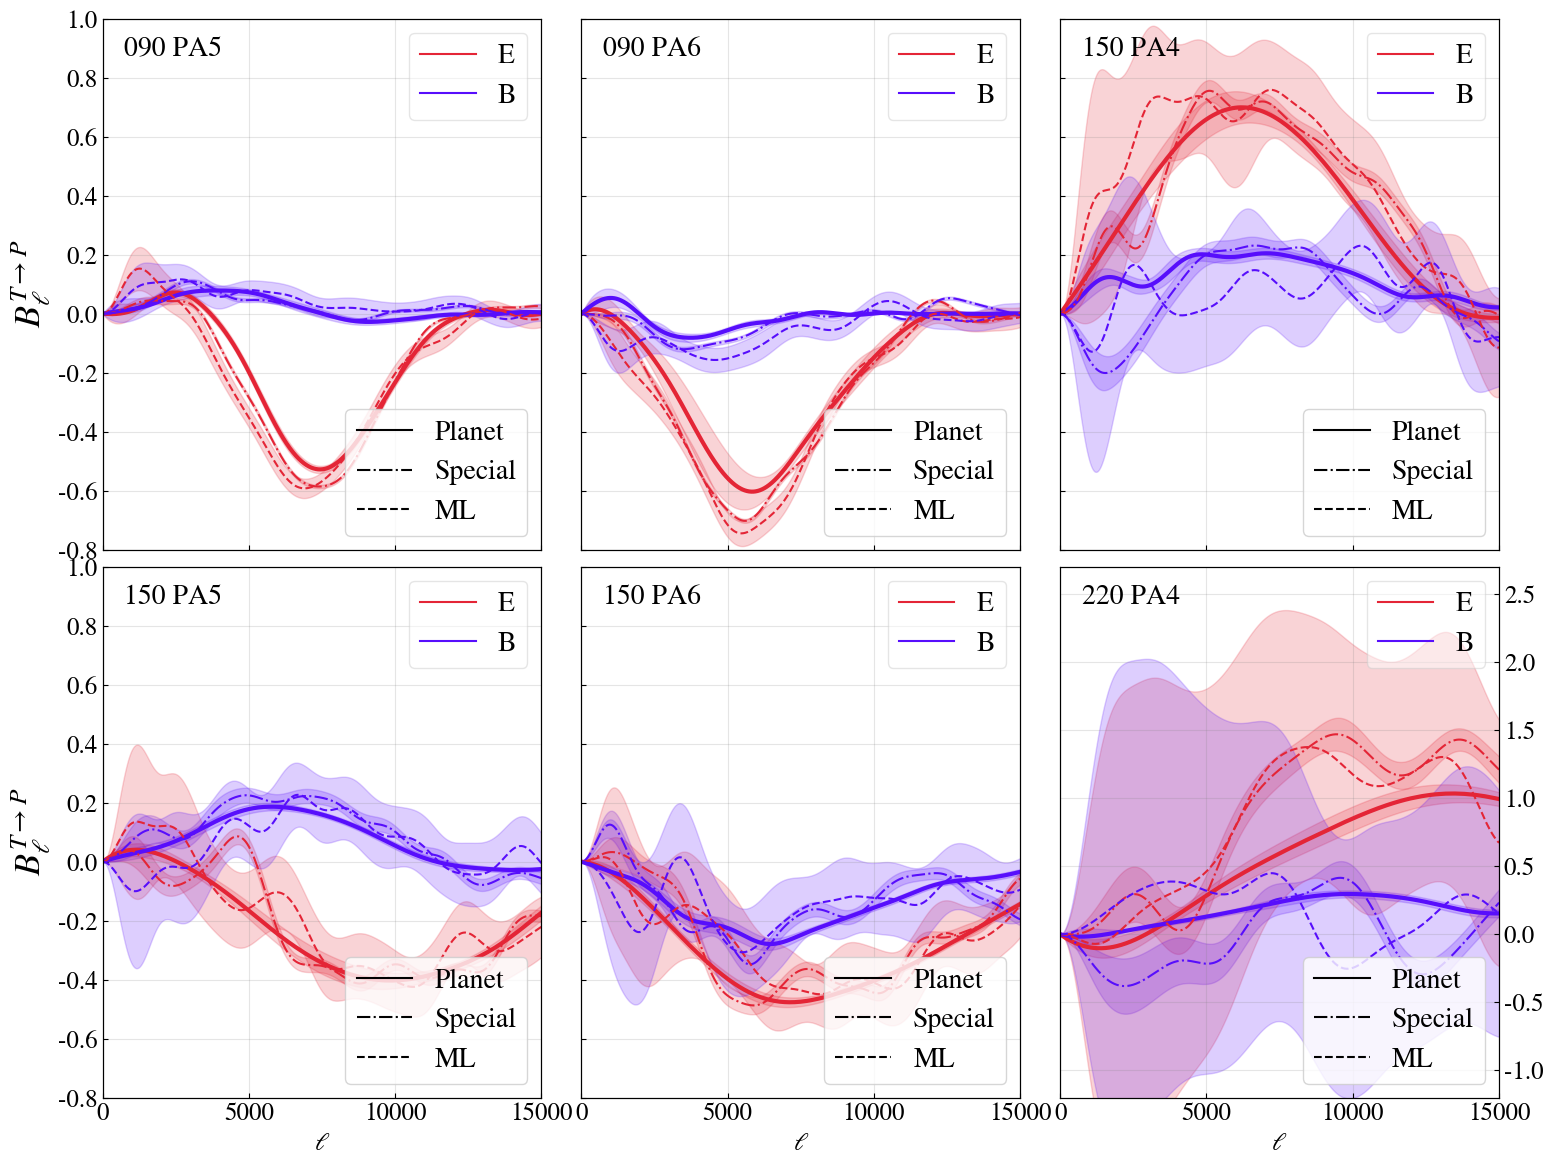
\includegraphics[width = \textwidth]{Figures/leakage.pdf}
    \caption{Polarization leakage, $B^{T\xrightarrow[]{}P}_{\ell}$, from stacked and Uranus-derived profiles.  Leakage beams are separated by Special(dashed-dotted) and ML(dashed) sources, with leakage from the planet profile(solid) plotted for comparison.  Stacked polarization leakage is consistent with leakage estimation from planet-derived profiles, indicating the planet profiles are a sufficient estimation for use on CMB maps.}
    \label{fig:leakage}
\end{figure*}

Figure~\ref{fig:polmodel} shows an example of the stacked polarization leakage beam, the modeled beam, and the residual for F150 PA4. Note that the quadrupole shape of the model is due to the reprojection onto the stack geometry: although we model the leakage beam as azimuthally symmetric when located on the pole of the standard spherical coordinate system, the symmetric shape turns into a quadrupole shape when rotated to the stack geometry location, which is centered on the equator. From the window functions, we obtain the window functions of each array's T$\xrightarrow[]{}$E and T$\xrightarrow[]{}$B leakage (Figure~\ref{fig:leakage}).

We find broad agreement between the Uranus-derived and stacked polarization beams.  This provides evidence that the planet-derived leakage estimation is appropriate for use in actual CMB maps.  Furthermore, there is no statistically significantly deviation between the Special and ML stacked leakage beam (any deviation is within the estimated error margin).

\section{Discussion}
\label{sec:act_disc}
In this paper, we have presented the analysis of the ACT beams for DR6 using a novel point source stacking method, which includes data from 2017--19.  We describe the full point-source stacking method, including the use of an inpainting method to remove large-scale structures and improve the signal-to-noise of the resulting stacked profiles.

The temperature beams show an increase in power at high $\ell$ scales when compared to the Uranus-derived profile, as well as a spatial variance when the stacks are separated by location on the sky.  This effect is especially significant for Special sources and requires further investigation to determine the exact source of such spatial variation.

Polarization leakage as determined by the stacks is not significantly different from the predicted leakage by the Uranus-derived profile.  Any difference of leakage between ML and Special profiles is within their respective error estimates, and therefore we consider them to be in agreement.  This indicates the planet-derived leakage estimation is sufficient for usage on CMB maps.

We believe point source stacking is a robust method for leakage estimation and instrument profile characterization.  This is especially useful to verify the planet-derived profiles commonly used to carry out cosmology science on CMB maps.

\chapter{Conclusion}
\label{ch:conclusion}

\appendix
\chapter{Open Source Holography} % Main appendix title
\label{app:holog}

\section{Open-Source Holography}
\label{sec:appendix_hardware}

Figure~\ref{fig:setup} shows a schematic of the RF electronics.  Two local oscillators (LOs) produce signals between 10 and 13 GHz. The LO1 synthesizer produces a signal between 10 and 13\,GHz, while LO2 produces the same frequency with some offset $f_{\text{offset}}$ (this offset is chosen to be 10\,MHz).  The offset frequency is what will eventually produce an intermediate frequency exiting the mixer diplexers.  The purpose of the mixer diplexers is to ensure the signal from the first LO travels to the two mixers, and then ensures that the IF output of the mixers travels in the opposing direction down the RF chain to the FPGA.

The LO1 signal goes to the active multiplying chain, where it is multiplied by 8(12), obtaining frequencies in the F90(150)-band.  Prior to leaving the source horn, -10dB of the signal splits off, and mixes with LO2 in the harmonic mixer, producing an intermediate frequency IF$_1$ which then goes through one of the mixer diplexers and to the FPGA.  The rest of the signal leaves the source horn, through the components of the LATR optics, and the signal reaching the back of the optics tube mixes with LO2 in a GaAs harmonic mixer, and the subsequent intermediate frequency, IF$_2$, which also travels to the FPGA.  The FPGA used for these measurements is the Re-configurable Open Architecture Computing Hardware (ROACH-2) board, which correlates the reference and modulated signals~\cite{roach2}.

\begin{figure}[ht]
    \centering
    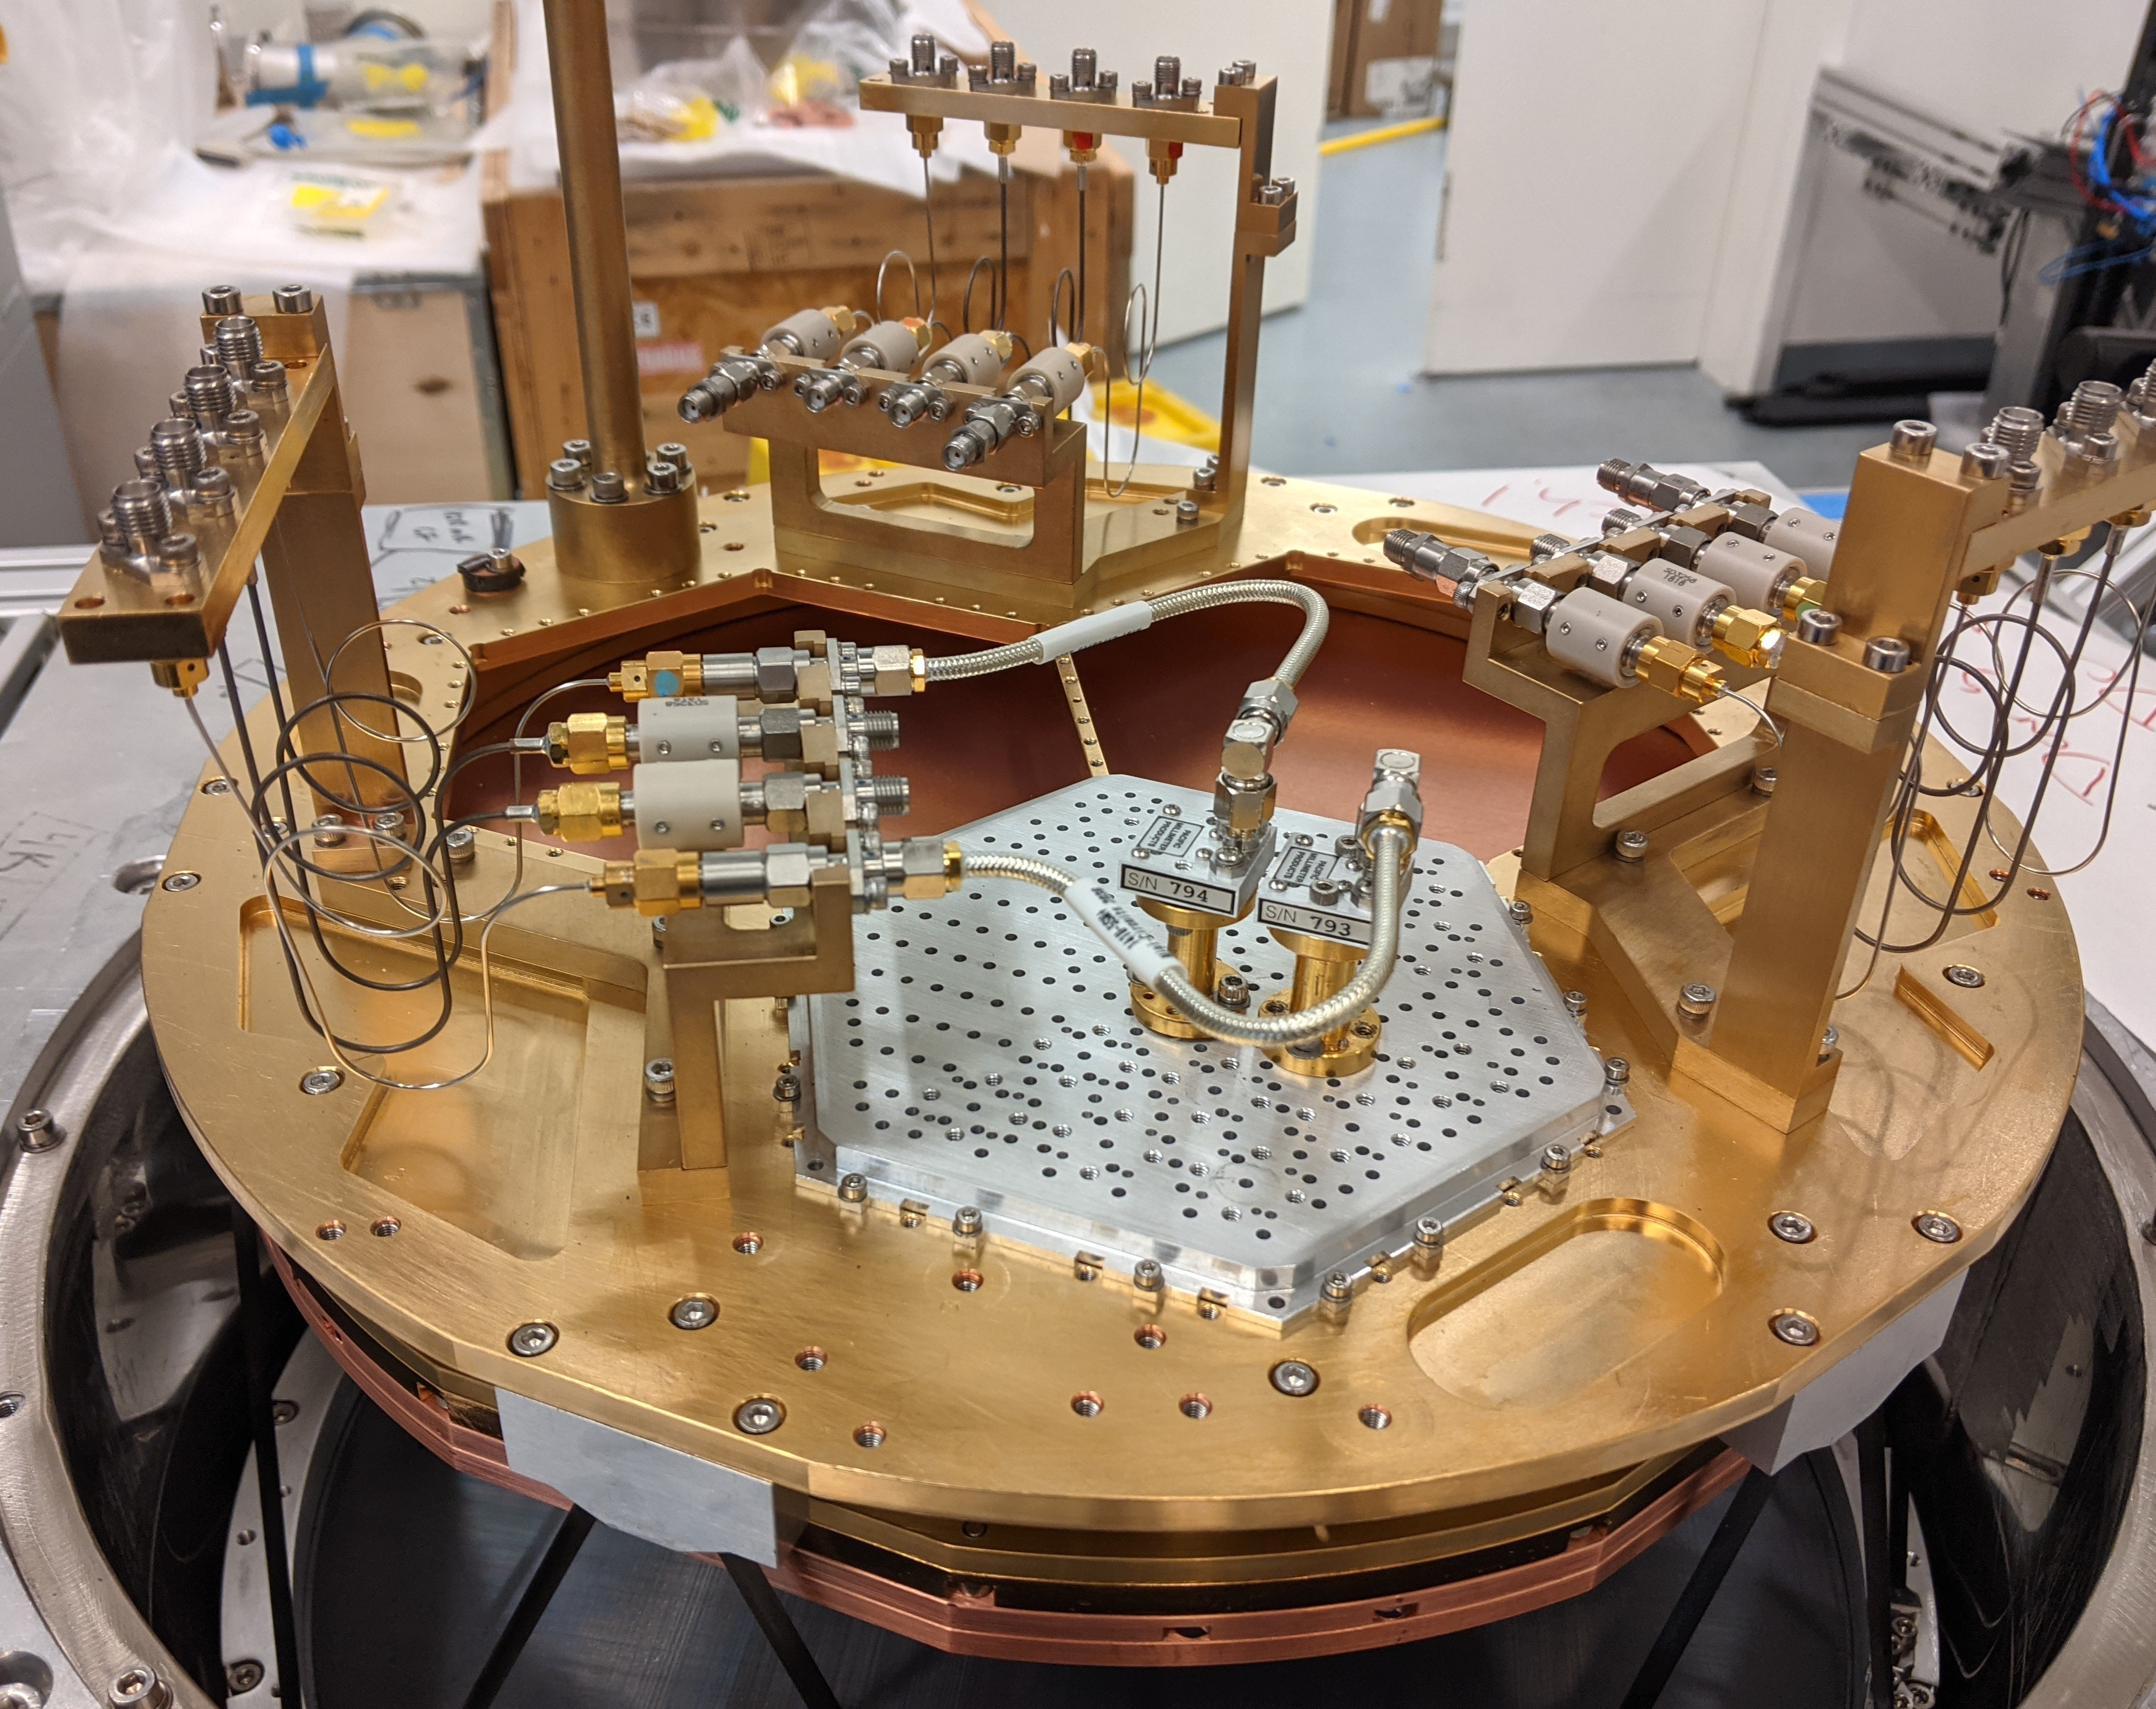
\includegraphics[width = .7\textwidth]{Figures/FPA.jpeg}
    \caption{The Simons Observatory Large Aperture Telescope optics tube focal plane readout, which is cooled to 4\,K during measurements.  The holography receivers (two receivers for redundancy) are approximately 7.4\,cm from the center of the focal plane.}
    \label{fig:fpa}
\end{figure}

The signal from the source(receiver) needs to be amplified due to high loss levels in the coax path from the harmonic mixer on the source to the reference mixer-diplexer (LATRt readout chain).  To overcome this loss, amplifiers with attenuators  increase the signal in the RF chain prior to entering the mixer diplexer.  The setup uses low phase variation coaxial cables leftover from the DASI experiment~\cite{CHURCH20031083}.  The phase repeatability of the holography setup is within $\approx3^{\circ}$.  We further note that any drift in the map would present itself in the phase map.  This phase drift would be removed during the propagation into the far-field when we optimize the position of the beam map in the LAT focal plane. 

The source moves in a 2-D grid above the LATRt with motorized XY stages~\cite{stages}.  The source mounts to the stages such that the signal points downwards towards the LATRt window.  The laboratory is over 7.5\,m tall, and therefore we expect reflection from the walls to be diffuse.  Therefore, the reflected signal is diluted before reflecting into the testing system.  The dominant reflections are from reflections within the optics tube, as the hexagon side-lobe is the dominant side-lobe feature in the beam maps (Figure~\ref{fig:beam_measurements_all}).
Figure~\ref{fig:fpa} shows the holography receiver readout at the back of the optics tube focal plane.  An SO MF feedhorn array is adapted for the holography experiment.  On the readout side of the array, attachment screws are added for attaching a circular to rectangular transition waveguide.  The transition waveguide connects the back of the focal plane (circular) to the GaAs W-band harmonic mixer (rectangular).  Though the design of the W-band harmonic mixer is optimized for F90 frequency readout, the W-band harmonic mixer is used for both F90 and F150 measurements (the entire SO MF band), allowing for a wider band of measurements without separate LATRt cool-downs.
\begin{figure*}[t!]
    \centering
    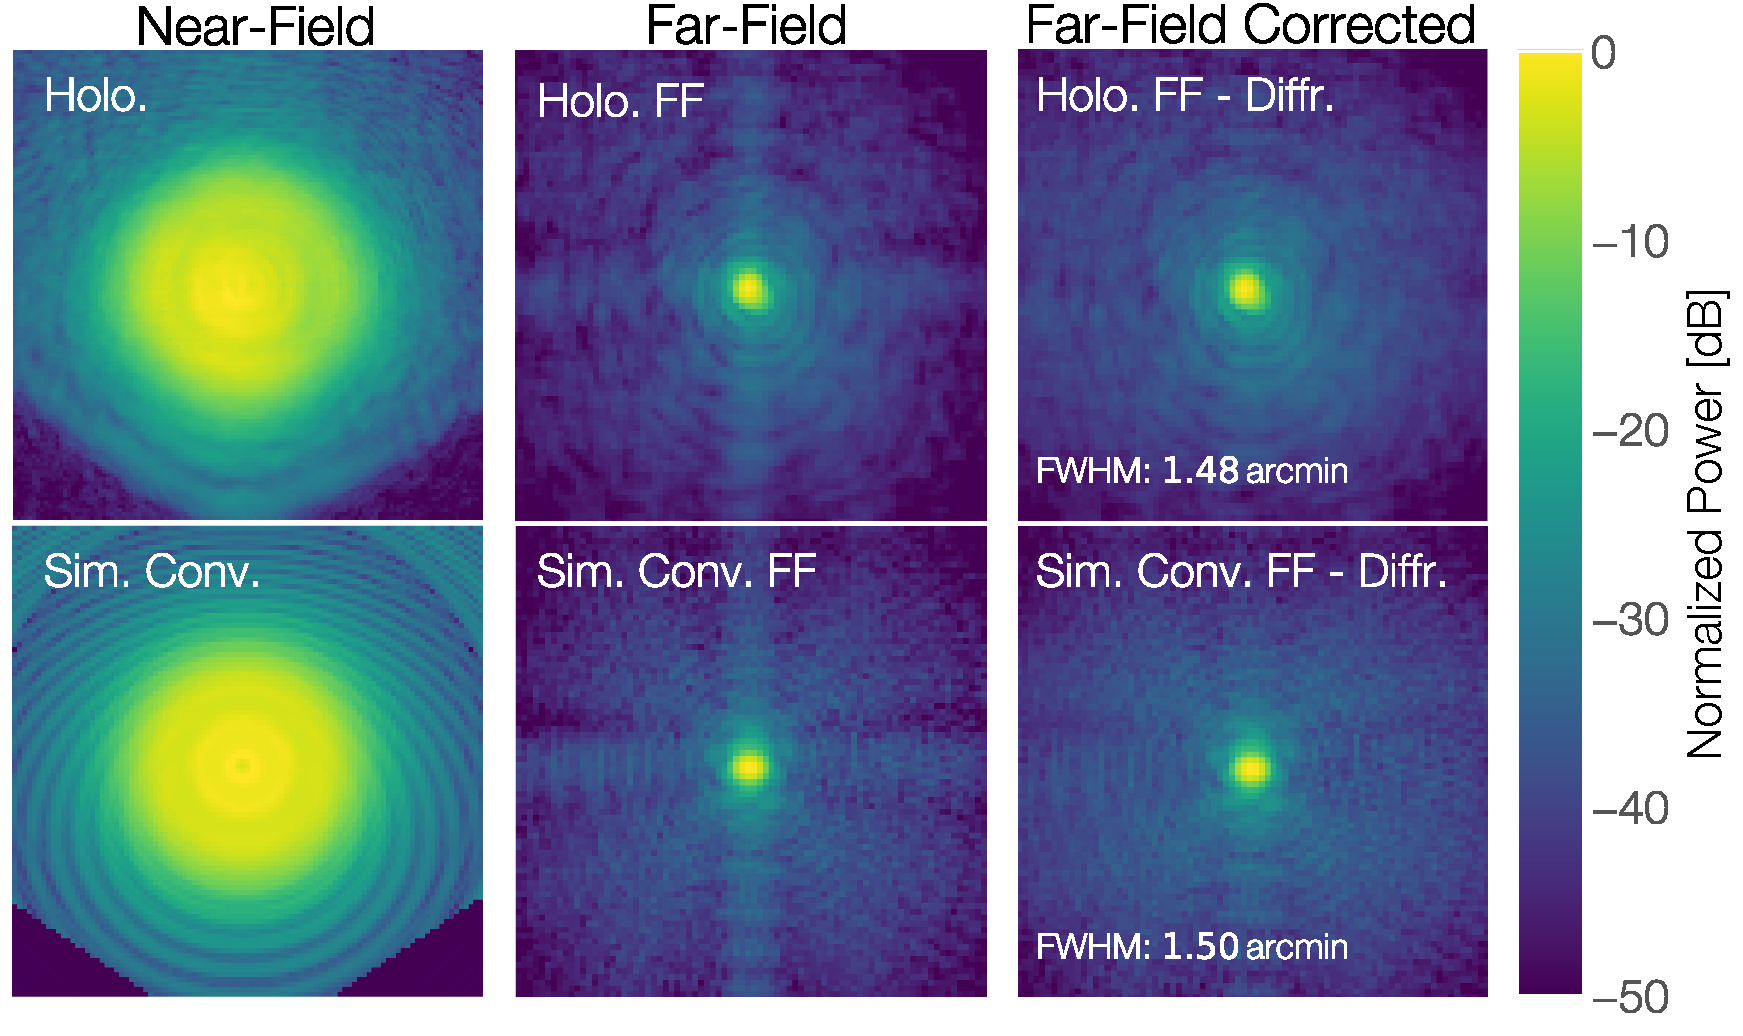
\includegraphics[width = .9\textwidth]{Figures/forward_convolve_highres.pdf}
    \caption{Forward modelling method with the F150 band-averaged holography data. Column 1:  Near-field holography data(top) and convolved simulation with a scattering term(bottom).  Square is $12\times12\,$cm.  Column 2: Far-field holography data(top) and convolved simulation with a scattering term(bottom).  Diffraction spikes consistent with a convolution from a square aperture are present in both the measured far-fields and the simulated far-fields, due to the source horn having a rectangular aperture face.  Square is $20\times20\,$arcmin.  Column 3:  Far-field holography data with diffraction model removal(top) and convolved simulation with a scattering term with diffraction model removal(bottom). Square is $20\times20\,$arcmin.}
    \label{fig:forward_model}
\end{figure*}
\section{Forward Modelling}
\label{sec:forward_model}
\begin{figure*}[t]
    \centering
    \includegraphics[width = .95\textwidth]{Figures/scatter_model.pdf}
    \caption{Simulated scattering term (power) in the near-field(left), at the secondary illumination(middle) and propagated to the far-field(right).  Each subplot is the band-averaged simulation over all F150 frequencies.}
    \label{fig:scattering_forward}
\end{figure*}
As introduced in Section~\ref{sec:results}.~\ref{sec:prop_fields}, the holography source emits from a rectangular feedhorn, and therefore result in a convolution of the electromagnetic field from the optics tube with the field pattern on the feedhorn aperture.  Convolving the simulated fields increases the F90(150) far-field beam by 12.2(4.7)\% and results in horizontal and vertical diffraction spikes in the raw far-field calculation~\cite{Goodman2005-ne}.

We carry out the forward modelling by building a simulation of the optics tube beam pattern at the measurement plane.  This model includes an empirical model of the scattering of the optics tube with the hexagonal outline to model the boundary of the optics tube window, and a similar amplitude and phase to what is measured.  The resulting simulated F90(150) beam matched the measured FWHP beam width within in 1.73(0.7)\%.  The simulation also had the horizontal and vertical diffraction spikes in the far-field due to the impact of the convolution with the holography source feed pattern~\cite{Goodman2005-ne}.  The full forward modelling process is shown in Figure~\ref{fig:forward_model}.
\begin{table}[ht]
\centering
\begin{tabular}{|c|c|c|c|c|}
\hline
F\,[GHz] & \multicolumn{3}{c|}{S/N [dB]}\\
& NF& Sec.& FF\\
\hline
 90      & 0 & 20.3  & 32.8\\
         & 20& 21.7 & \\
         & 40& 37.0 & \\
         & 60& 45.4 & \\
 150     & 0 & 15.0 & 32.3 \\
         & 20& 18.0 & 39.3\\
         & 40& 35.5 & 43.8\\
         & 60& 46.0 & 43.8\\
 \hline
\end{tabular}
\caption{Near-field measurement signal-to-noise and resulting far- side-lobe power (at the secondary illumination and into the far-field).}
\label{tab:fft_sn}
\end{table}
For visualization purposes, these spikes are removed by subtracting a model $D(\theta_x,\theta_y)$ (amplitude of the electric field) consisting of a $\sinc$ function with a Gaussian width along its narrow direction equal to the beam width (Eq.~\ref{eq:model_conv}), where $\theta_x$ and $\theta_y$ are elevation and azimuth, and we fit the 2 parameters $\sigma_{\theta_x}$ and $\sigma_{\theta_y}$.  This model is based on the predicted Fraunhofer diffraction pattern from a rectangular aperture~\cite{Goodman2005-ne} (e.g., the feed) and was shown to match the simulations.
\begin{equation}
    D(\theta_x,\theta_y) = \exp^{-(\theta_x^2/4\sigma_{\theta_x}^2 +\theta_y^2/4\sigma_{\theta_y}^2 )}\sinc{\theta_x}\sinc{\theta_y}
    \label{eq:model_conv}
\end{equation}
The holography measurements showed scattering from within the optics tube (hexagonal shape at ~-20\,dB in Figure~\ref{fig:beam_measurements_all}).  To understand how this scattering propagates through the telescope, we add a scattering term (with both amplitude and phase) to the simulated beam, and then propagate this beam into the far-field.  We also investigate how the side-lobes measured outside the main beam (Fig.~\ref{fig:beam_measurements_all}) propagate into the far-field (Fig.~\ref{fig:scattering_forward}).  Reflections are known to be a problem in near-field beam mapping~\cite{2020JLTP..199..156Y,7740846,387181}.  However, the inferred amplitude of the probe is small, and we do not correct for reflections.  The side-lobe spreads out and is localized to 2 meters from the center of the primary and secondary mirrors, and then leads to a $0.85^{\circ}$ diffuse structure on the sky that is at the $\approx -15$\,dBi level.
\section{Measurement Requirements}
\label{sec:err_prop}
Here, we discuss the measurement requirements to meet specific far-field resolution from near-field data.  Near-field beams with four signal-to-noise levels are propagated into the far-field (for 90\, and 150\,GHz near-field beams); we simulate the near-fields to have 0, 20, 40, and 60\,dB signal-to-noise.  The signal-to-noise propagated to the secondary illumination and to the far-field is listed in Table~\ref{tab:fft_sn}. 
\begin{table}[htb]
\centering
\begin{tabular}{|c|c|c|c|c|c|c|}
\hline
F\,[GHz] & \multicolumn{2}{c|}{NF [cm]}&\multicolumn{2}{c|}{Sec. [m]} & \multicolumn{2}{c|}{FF [arcmin]} \\
 & Size & Res. & Size & Res.& Size & Res.\\ \hline
 90 & 50& 0.25 & 9.52& 0.13& 119.72 & 0.60\\
 150 & 50& 0.20 &6.66 &0.06 &128.40&0.52\\
 \hline
\end{tabular}
\caption{Near-field scan size and resolution, and resulting scan size and resolution at the secondary illumination and in the far-field.}
\label{tab:fft_grid}
\end{table}
When planning the near-field scan, we consider the resolution and how the near-field grid propagates into the far-field, due to the Fourier relationship between near- and far-fields (Eq.~\ref{eq:fft}).  Table~\ref{tab:fft_grid} summarizes the scan size and resolutions and resulting far-field size and resolution grids used in the holography measurements.

% Appendix Template

\chapter{Holography Receiver Polarization Through the Large Aperture Telescope Optics Tube} % Main appendix title
\label{app:pol} % Change X to a consecutive letter; for referencing this appendix elsewhere, use \ref{AppendixX}

Here, I derive each component of the polarization modulation using Mueller matrix notation~\cite{MUELLER}.  This model is used to fit the measured response through a polarized grid in the LATR tester optics tube, using the same holography receiver.  The electric field measured by the detector $\vec{E}_{\text{det}}$ can be modelled as a series of polarization modulations: 
\begin{equation}
    \vec{P}_{\text{out}}(\theta) = \vec{S}_{\text{det}}(\phi_{\text{det}},\epsilon)\cdot \vec{M}_{\text{OT}}\cdot \vec{M}_{\text{grid}}(\theta,\eta_{g})\cdot \vec{S}_{\text{source}}
    \label{eq:holo_model}
\end{equation}
where the source emits the field $\vec{E}_{\text{source}}$, which is then modulated by the grid $\vec{M}_{\text{grid}}$.  The field then enters the optics tube $\vec{M}_{\text{OT}}$ and is measured by the detector $\vec{M}_{\text{det}}$.  These data were used to quantify the grid efficiency $\eta_{\text{Grid}}$, the cross-polarization of the instrument $CP$, and the tilt-offset of the holography detector $\theta_{\text{det}}$.

\section{General Notation}
\subsection{Stokes Parameters}
\begin{equation}
\begin{split}
    I & = |E_x|^2 + |E_y|^2 \\
    Q & = |E_x|^2 - |E_y|^2 \\
    U & = E_x E_y^* + E_x^*E_y\\
    V & = i(E_x E_y^* - E_x^*E_y) \\
\end{split}
\end{equation}

\subsection{Jones into Mueller Matrix}
Convert from Jones to Mueller matrices with:
\begin{equation}
    M = A(J\otimes J^*)A^{-1}
\end{equation}
where
\begin{equation}
    A = \begin{bmatrix}
    1 & 0 & 0 & 1\\
    1 & 0 & 0 & -1\\
    0 & 1 & 1 & 0\\
    0 & -i & i & 0\\
  \end{bmatrix}\quad\text{and}\quad 
     A^{-1} = \frac{1}{2}\begin{bmatrix}
    1 & 1 & 0 & 0\\
    0 & 0 & 1 & i\\
    0 & 0 & 1 & -i\\
    1 & -1 & 0 & 0\\
  \end{bmatrix}
\end{equation}



\section{Mueller Matrices}

Here we list the individual matrices which make up the full model of the measurement.  We use Mueller matrices to modulate the polarization of the holography source $\vec{S}_{co,cr}$.  To rotate into a given component's coordinate system, we employ the Mueller rotation matrix:

\begin{equation}
   M_{\text{rot}}= \begin{bmatrix}
    1 & 0 & 0 & 0 \\
    0 & \cos{2\theta} & \sin{2\theta} & 0 \\
    0 & -\sin{2\theta} & \cos{2\theta} & 0  \\
    0 & 0 & 0 & 1
    \end{bmatrix}
\end{equation}

\subsection{Polarized Source}
The holography source is linearly polarized (TM-mode).  We model the source as a general polarized source.  The Stokes parameters of a linearly polarized source along the $\theta=0^\circ$ axis:
\begin{equation}\vec{S}_{co} = 
    \begin{bmatrix}
    1 & 1 & 0 & 0
    \end{bmatrix}^T
\end{equation}
    
The second source polarization was obtained by adding a waveguide twist directly onto the source's output, prior to the rectangular horn.  Therefore, the Stokes parameters of the source in the $\theta=90^\circ$ axis is modeled as:
\begin{equation}\vec{S}_{cr} = 
    \begin{bmatrix}
    1 & -1 & 0 & 0
    \end{bmatrix}^T
\end{equation}

\subsection{Polarizing Grid}
The signal is first modulated by the polarized grid prior to entering the optics tube.  The purpose of the grid is to transmit one polarization and reflect the other.  However, in the case of an imperfect polarizing grid, some of the $2^{nd}$ polarization may also transmit (a fraction of the $1^{st}$ polarization).  Therefore, we define the Jones matrix as the following, where the majority of the signal along the $x$-axis is transmitted ($t_x > t_y$):
\begin{equation}
    J_{\text{grid}} = \begin{bmatrix}
    t_x & 0 \\
    0 & t_y\\
  \end{bmatrix}
\end{equation}
where $t_x\approx 1$ and $t\approx 0 $.  Now, as before, we convert to the grid's Mueller matrix:
\begin{equation}
    M_{\text{grid}} =\frac{1}{2} \begin{bmatrix}
    |t_x|^2 + |t_y|^2 & |t_x|^2 - |t_y|^2 & 0& 0\\
    |t_x|^2 - |t_y|^2 & |t_x|^2 + |t_y|^2& 2\Re{(t_x t_y^*)}& -2\Im{(t_x t_y^*)}\\
    0 & 0& 2\Im{(t_x t_y^*)}& 2\Re{(t_x t_y^*)}\\
  \end{bmatrix}
\end{equation}
The efficiency of our wire grid is defined by the transmission through the $x$-axis $t_x$. We want to determine the grid efficiency from our data, so we can re-write our Mueller matrix as:
\begin{equation}
    M_{\text{grid}} =\frac{1}{2} \begin{bmatrix}
    1 & \eta_g & 0& 0\\
    \eta_g & 1& 1-\eta_g^2 & -\sqrt{1-\eta_g^2}\\
    0 & 0& \sqrt{1-\eta_g^2}& \sqrt{1-\eta_g^2}\\
  \end{bmatrix}
\end{equation}

Lastly, we rotate the grid via the $M_{\text{rot}}(\theta)$ matrices:

\begin{equation}
    M_{\text{grid}}(\theta,\eta_{g}) = M_{\text{rot}}^T(\theta) \cdot M_{\text{grid}}(\eta_{g})\cdot M_{\text{rot}}(\theta)
\end{equation}


\subsection{Generic Instrument}
\begin{equation}
    J = \begin{bmatrix}
    1 & 0 \\
    0 & A e^{i\phi}\\
  \end{bmatrix}
\end{equation}

Converting this to a Mueller matrix yields:

\begin{equation}
    M_{\text{IP}} = \frac{1}{2}\begin{bmatrix}
    1+A^2 & 1-A^2 & 0& 0\\
    1-A^2 & 1+A^2 & 0& 0\\
    0 & 0 & 2A\cos\phi & 2A\sin\phi\\
    0 & 0 & -2A\sin\phi & 2A\cos\phi
  \end{bmatrix}
\end{equation}

We define the instrument's polarization as $\lambda_P = \frac{1}{2}\sqrt{1-A^2}$.  Here's we only consider $\phi=0$ or else we would find $A<1$, which isn't physical in our setup.  Our Mueller matrix becomes:

\begin{equation}
    M_{\text{IP}} = \frac{1}{2}\begin{bmatrix}
    1-\lambda_P & \lambda_P & 0& 0\\
    \lambda_P & 1-\lambda_P & 0& 0\\
    0 & 0 & \sqrt{1-2\lambda_P} & 0\\
    0 & 0 & 0 & \sqrt{1-2\lambda_P}
  \end{bmatrix}
\end{equation}

Our model for instrument polarization is aligned along a specific axis, so we need to rotate this matrix into the appropriate local coordinate system via the rotation matrix $M_{rot}$.

\subsection{Detector}

We model the detector as an imperfect polarizer, to include any small cross-polarization from the receiver:
\begin{equation}
    J_{\text{det}} = \begin{bmatrix}
    1 & 0 \\
    0 & \epsilon\\
  \end{bmatrix}
\end{equation}

The Mueller matrix then becomes:
\begin{equation}
    M_{\text{det}} = \begin{bmatrix}
    1 & 0 \\
    0 & \epsilon\\
  \end{bmatrix}
\end{equation}

We need to rotate this polarization matrix by the tilt of the detector $\phi$ via:
\begin{equation}
    \vec{E}_{\text{det}} = M_{\text{det}}\cdot M_{\text{rot}}(\phi)
\end{equation}

Because the power out from the detector $P_{\text{out}}$ is the $I$ component of the Stoke's parameters, we then get the final $\vec{S}_{\text{out}}$ with:

\begin{equation}
    \vec{S}_{\text{det}} = \begin{bmatrix}
    1 & 0 & 0 & 0
  \end{bmatrix} \cdot M_{\text{det}} \cdot M_{\text{rot}}(\phi)
\end{equation}

% \chapter{Polarized Beam Transformation Formalism} % Main appendix title
\label{app:act} 

Here, we derive the locally defined map-space polarization basis to determine the polarized $\ell$-space beams from the $Q$ and $U$ beams.  The basis of $Q_r$ and $U_r$ are defined as local linear combinations of the $Q$ and $U$ maps as:
\begin{equation} \label{eq:q_r}
\begin{split}
    Q_r(\boldsymbol{\theta}) =& Q(\boldsymbol{\theta}) \cos 2\phi_{\theta} + U(\boldsymbol{\theta}) \sin 2\phi_{\theta} \\
    U_r(\boldsymbol{\theta}) =& U(\boldsymbol{\theta}) \cos 2\phi_{\theta} - Q(\boldsymbol{\theta}) \sin 2\phi_{\theta}
\end{split}
\end{equation}
where $\boldsymbol{\theta} \equiv (\theta,\phi_\theta)$ are standard polar coordinates with the beam's center as their origin and $\phi_{\theta}$ increasing clockwise from the positive $y$-axis (assuming $+x$ points to the right and $+y$ points upward).  We can also define these fields conversely:
\begin{equation} \label{eq:q}
\begin{split}
    Q(\boldsymbol{\theta}) =& Q_r(\boldsymbol{\theta}) \cos 2\phi_{\theta} - U_r(\boldsymbol{\theta}) \sin 2\phi_{\theta} \\
    U(\boldsymbol{\theta}) =& U_r(\boldsymbol{\theta}) \cos 2\phi_{\theta} + Q_r(\boldsymbol{\theta}) \sin 2\phi_{\theta} \; .
\end{split}
\end{equation}
In order to determine beam leakage in the angular power spectra, we need to translate the polarized beams $Q_r$ and $U_r$ to the $\ell$-space $E$ and $B$ polarized beams.  To do so, we employ the relation between the azimuthally averaged versions of each component, derived here in the flat-sky limit.  The Fourier-space expressions for $E$ and $B$ are:
\begin{equation} \label{eq:e}
\begin{split}
        E(\boldsymbol{\ell}) =& \hat{Q}(\boldsymbol{\ell}) \cos 2\phi_{\ell} + \hat{U}(\boldsymbol{\ell}) \sin 2\phi_{\ell}\\
        B(\boldsymbol{\ell}) =& \hat{U}(\boldsymbol{\ell}) \cos 2\phi_{\ell} - \hat{Q}(\boldsymbol{\ell}) \sin 2\phi_{\ell}
\end{split}
\end{equation}
where $\boldsymbol{\ell} \equiv (\ell,\phi_\ell)$ is the Fourier conjugate of $\boldsymbol{\theta}$, and $\{\hat{Q},\hat{U}\}$ are the standard Fourier transforms of $\{Q,U\}$:
\begin{equation} \label{eq:q_hat}
\begin{split}
        \hat{Q}(\boldsymbol{\ell}) =& \int Q(\boldsymbol{\theta}) e^{i\boldsymbol{\ell}\cdot\boldsymbol{\theta}} d\boldsymbol{\theta} = \int Q(\theta,\phi_{\theta}) e^{i\ell\theta\cos(\phi_{\theta} - \phi_\ell)} \theta\; d\theta\; d\phi_{\theta} \\
        \hat{U}(\boldsymbol{\ell}) =& \int U(\boldsymbol{\theta}) e^{i\boldsymbol{\ell}\cdot\boldsymbol{\theta}} d\boldsymbol{\theta} = \int U(\theta,\phi_{\theta}) e^{i\ell\theta\cos(\phi_{\theta} - \phi_{\ell})} \theta\; d\theta\; d\phi_{\theta} \; .
\end{split}
\end{equation}

Taking the azimuthal average of Equations \ref{eq:e} gives the one-dimensional transforms $\tilde{E}$ and $\tilde{B}$:
\begin{equation} \label{eq:tilde_e1}
\begin{split}
    \tilde{E}(\ell) =& \frac{1}{2\pi} \int \hat{Q}(\boldsymbol{\ell}) \cos 2\phi_{\ell}\;d\phi_{\ell} + \frac{1}{2\pi} \int \hat{U}(\boldsymbol{\ell}) \sin 2\phi_{\ell}\;d\phi_{\ell}   \\
    \tilde{B}(\ell) =& \frac{1}{2\pi} \int \hat{U}(\boldsymbol{\ell}) \cos 2\phi_{\ell}\;d\phi_{\ell} - \frac{1}{2\pi} \int \hat{Q}(\boldsymbol{\ell}) \sin 2\phi_{\ell}\;d\phi_{\ell} \; .    
\end{split}
\end{equation}
We can re-write the expression for $\tilde{E}$ in Equation \ref{eq:tilde_e1} in terms of map-space $Q$ and $U$ by using Equations~\ref{eq:q_hat} (from here on we derive only for $E$ but $B$ can be derived identically):
\begin{equation} \label{eq:tilde_e2}
\begin{split}
        \tilde{E}(\ell) = & \frac{1}{2\pi} \int Q(\theta,\phi_{\theta}) e^{i\ell\theta\cos(\phi_{\theta} - \phi_{\ell})} \theta\;d\theta\;d\phi_{\theta} \cos 2\phi_{\ell}\;d\phi_{\ell} \\ &
    + \frac{1}{2\pi} \int U(\theta,\phi_{\theta}) e^{i\ell\theta\cos(\phi_{\theta} - \phi_{\ell})} \theta\;d\theta\;d\phi_{\theta} \sin 2\phi_{\ell}\;d\phi_{\ell} \; .
\end{split}
\end{equation}

Substituting for $Q(\boldsymbol{\theta})$ and $U(\boldsymbol{\theta})$ in Equation \ref{eq:tilde_e2} using Equations in \ref{eq:q}, we find the relation between $\tilde{E}$ and $\{Q_r,U_r\}$:
\begin{equation} \label{eq:tilde_e3}
\begin{split}
    \tilde{E}(\ell) = & \frac{1}{2\pi} \int \big(Q_r(\theta,\phi_{\theta})\cos 2\phi_{\theta} - U_r(\theta,\phi_{\theta})\sin 2\phi_{\theta}\big) e^{i\ell\theta\cos(\phi_{\theta} - \phi_{\ell})} \theta\;d\theta\;d\phi_{\theta} \cos 2\phi_{\ell}\;d\phi_{\ell} \\ & 
    + \frac{1}{2\pi} \int \big(U_r(\theta,\phi_{\theta})\cos 2\phi_{\theta} + Q_r(\theta,\phi_{\theta})\sin 2\phi_{\theta}\big) e^{i\ell\theta\cos(\phi_{\theta} - \phi_{\ell})} \theta\;d\theta\;d\phi_{\theta} \sin 2\phi_{\ell}\;d\phi_{\ell}\; .
\end{split}
\end{equation}
Now grouping terms together with $Q_r(\boldsymbol{\theta})$ and $U_r(\boldsymbol{\theta})$, we re-write the above equation and find:
\begin{equation} \label{eq:tilde_e4}
\begin{split}
    \tilde{E}(\ell) = & \frac{1}{2\pi} \int Q_r(\theta,\phi_{\theta})\big(\cos 2\phi_{\theta} \cos 2\phi_{\ell} + \sin 2\phi_{\theta} \sin 2\phi_{\ell}\big) e^{i\ell\theta\cos(\phi_{\theta} - \phi_{\ell})} \theta\;d\theta\;d\phi_{\theta}\;d\phi_{\ell} \\ &
    + \frac{1}{2\pi} \int U_r(\theta,\phi_{\theta})\big(\cos 2\phi_{\theta} \sin 2\phi_{\ell} - \sin 2\phi_{\theta} \cos 2\phi_{\ell}\big) e^{i\ell\theta\cos(\phi_{\theta} - \phi_{\ell})} \theta\;d\theta\;d\phi_{\theta}\;d\phi_{\ell}\; .
\end{split}
\end{equation}
Then, making use of the trigonometric identity:
\begin{equation}
    \begin{split}
        \cos(\alpha\pm\beta) =& \cos\alpha\cos\beta \mp \sin\alpha\sin\beta \\
        \sin(\alpha\pm\beta) =& \sin\alpha\cos\beta \mp \cos\alpha\sin\beta
    \end{split}
\end{equation}
...Equation \ref{eq:tilde_e4} may be re-written as:
\begin{equation} \label{eq:tilde_e5}
\begin{split}
    \tilde{E}(\ell) = & \frac{1}{2\pi} \int Q_r(\theta,\phi_{\theta})\cos 2(\phi_{\theta}-\phi_{\ell})\;e^{i\ell\theta\cos(\phi_{\theta} - \phi_{\ell})} \theta\;d\theta\;d\phi_{\theta}\;d\phi_{\ell} \\ &
    - \frac{1}{2\pi} \int U_r(\theta,\phi_{\theta})\sin 2(\phi_{\theta}-\phi_{\ell})\;e^{i\ell\theta\cos(\phi_{\theta} - \phi_{\ell})} \theta\;d\theta\;d\phi_{\theta}\;d\phi_{\ell} \; .
\end{split}
\end{equation}
To simplify this, we define $\phi_{\rho} \equiv \phi_{\theta} - \phi_{\ell}$, and Equation \ref{eq:tilde_e5} becomes:
\begin{equation} \label{eq:tilde_e6}
\begin{split}
    \tilde{E}(\ell) = & \frac{1}{2\pi} \int Q_r(\theta,\phi_{\theta})\cos 2\phi_{\rho}\;e^{i\ell\theta\cos\phi_{\rho}}\;\theta\;d\theta\;d\phi_{\theta}\;d\phi_{\rho}\\ &
    - \frac{1}{2\pi} \int U_r(\theta,\phi_{\theta})\sin 2\phi_{\rho}\;e^{i\ell\theta\cos\phi_{\rho}}\;\theta\;d\theta\;d\phi_{\theta}\;d\phi_{\rho}\; .
\end{split}
\end{equation}
Each of the two terms in Equation~\ref{eq:tilde_e6} can be expressed as three separate integrals:
\begin{equation} \label{eq:sep_int}
\begin{split}
    \tilde{E}(\ell) = & \int \big(\frac{1}{2\pi} \int Q_r(\theta,\phi_{\theta})\,d\phi_{\theta}\big) \big(\int \cos 2\phi_{\rho}\;e^{i\ell\theta\cos\phi_{\rho}}\;d\phi_{\rho}\big) \theta\;d\theta \\ & - \int \big(\frac{1}{2\pi} \int U_r(\theta,\phi_{\theta})\;d\phi_{\theta}\big) \big(\int \sin 2\phi_{\rho}\;e^{i\ell\theta\cos\phi_{\rho}}\;d\phi_{\rho}\big) \theta\;d\theta \; .
\end{split}
\end{equation}
Conveniently, the integrals of $Q_r(\boldsymbol{\theta})$ and $U_r(\boldsymbol{\theta})$ over $\phi_{\theta}$ are the azimuthal averages of $Q_r$ and $U_r$.  The integrals over $\phi_{\rho}$ - the second set of parentheses - turn out to have simple analytic counterparts:
\begin{equation}
    \int \cos 2\phi_{\rho}\;e^{i\ell\theta\cos\phi_{\rho}}\;d\phi_{\rho} = -2\pi J_2(\ell\theta)
\end{equation}
\begin{equation}
    \int \sin 2\phi_{\rho}\;e^{i\ell\theta\cos\phi_{\rho}}\;d\phi_{\rho} = 0 \; .
\end{equation}
Plugging these into our expressions for $\tilde{E}(\ell)$, the azimuthally averaged $\ell$-space $E$ beam is simply the second-order Hankel transform of the azimuthally averaged map-space $Q_r$ beam:
\begin{equation} \label{eq:final1}
    \tilde{E}(\ell) = -2\pi\int \tilde{Q}_r(\theta) J_2(\ell\theta)\;\theta\;d\theta \; .
\end{equation}
While the same relation exists between the azimuthally averaged $\ell$-space $B$ and map-space $U_r$ beams:
\begin{equation} \label{eq:final2}
    \tilde{B}(\ell) = -2\pi\int \tilde{U}_r(\theta) J_2(\ell\theta)\;\theta\;d\theta \; .
\end{equation}
The final Equations \ref{eq:final1} and \ref{eq:final2} provide a complete formalism for transforming the polarized beams using the $\{Q_r,U_r\}$ basis.

\chapter{Harmonic Transform of the Beam} % Main appendix title
\label{app:trans} 

Here we show the derivation to convert our beam $B(\theta)$ to its spherical transform $b_\ell$. The spherical harmonics are functions defined on the sphere as
\begin{equation}
    Y_l^m(\theta,\phi) = P_l^m(\cos\theta)\exp{i m\phi} \; ,
\end{equation}
where $P_l^m$ are the Legendre polynomials normalized for spherical harmonics, $\ell$ and $m$ are multipoles, and $\theta$ and $\phi$ are standard sky coordinates. The Legendre polynomials are defined as:
\begin{equation}
    P_l^m(x) = (-1)^m\sqrt{\frac{2l+1}{4\pi}}\sqrt{\frac{(l-\abs{m})!}{(l+\abs{m})!}}(1-x^2)^{\abs{m}/2}\frac{d^{\abs{m}}}{dx^{\abs{m}}}P_l(x) \; .
\end{equation}
The spherical harmonics are orthonormal, and thus obey the relation
\begin{equation}
    \int_0^{2\pi}\int_0^{\pi} Y_l^m(\theta,\phi)\overline{Y_{l'}^{m'}}(\theta,\phi) \sin\theta \; d\theta\; d\phi = \delta_{ll'}\delta_{mm'} \; ,
\end{equation}
where $\overline{z}$ is the complex conjugate of $z$ and $\delta_{ij}$ is the Kronecker symbol.

In a spherical harmonic transform, we compute the coefficients $f_{l}^{m}$ used to express a function $f (\theta,\phi)$ as
\begin{equation}
    f(\theta,\phi) = \sum_{l=0}^{\infty}\sum_{m=-l}^{l}f_{l}^{m} Y_l^m(\theta,\phi) \; .
\end{equation} 
The coefficients can be computed using the equation 
\begin{subequations}
\begin{align}
    f_{l}^{m} &= \int_{0}^{2\pi}\int_{0}^{\pi} f(\theta,\phi) \overline{Y_l^m}(\theta,\phi)\sin\theta \; d\theta\; d\phi   \\
    & = \int_{0}^{2\pi}\int_{0}^{\pi} f(\theta,\phi) P_{l}^{m}(\cos\theta)\exp{-im\phi} \sin\theta\; d\theta\; d\phi \; .
\end{align}
\end{subequations}
If $f (\theta,\phi)$ is independent of $\phi$ (as is the case for our beam), then we can write $f (\theta,\phi)$ = $f (\theta)$ and the equation above becomes
\begin{equation}
    f_{l}^{m}= \int_{0}^{2\pi}\exp{-im\phi}d\phi\int_{0}^{\pi} f(\theta) P_{l}^{m}(\cos\theta) \sin\theta\; d\theta \; .
\end{equation}
The integral over $\phi$ then simplifies to 
\begin{equation}
    \int_0^{2\pi} e^{-im\phi}\; d\phi = 2\pi \delta_{m0}\; .
\end{equation}
So $f_l^m$ is only non-zero for $m=0$, in which case we have 
\begin{subequations}
\begin{align}
    f_l^0 & =  2\pi\int_0^{\pi}f(\theta)P_l(\cos\theta)\sin\theta \; d\theta\\
    & = 2\pi \int_{-1}^{1}f(\theta)P_l (\cos\theta) \; d\cos \theta\; .
\end{align}
\end{subequations}
This is the equation for the Legendre polynomial transform, presented as a means of converting the radial beam profile $B(\theta)$ to the harmonic transform $B_{\ell}$. 

% However, this can be time-consuming to compute. For small beams such as ours, it is not necessary to work in the curved sky regime. We instead perform a 2D Fourier transform, which effectively becomes a Hankel transform, as shown below. The difference between the Hankel and Legendre polynomial transforms is less than a factor of $4\times 10^{-5}$ between $\ell=0$ and $\ell=10,000$ and the Hankel transform is much faster to compute. 

% Now let's consider the 2D Fourier transform of a function $f(x,y)$, 
% \begin{equation}
%     F(k_x,k_y) = \int_{-\infty}^{\infty}\int_{-\infty}^{\infty}f(x,y)\exp{-i(xk_x+ yk_y)}\;dx\; dy \; .
% \end{equation}
% Introducing the polar coordinates
% \begin{equation*}
%     \begin{split}
%     x = \theta\cos\phi \hspace{0.5cm}& \hspace{0.5cm} y = \theta\sin\phi\\
%     k_x = k\cos\psi \hspace{0.5cm}& \hspace{0.5cm} k_y = k\sin\psi
%     \end{split}
% \end{equation*}
% where $\theta$ and $\phi$ here correspond to the $\theta$ and $\phi$ in spherical coordinates used throughout the paper, we then have, in the flat sky approximation,
% \begin{equation}
%         F(k\cos\psi,k\sin\psi) \equiv \mathcal{F}(k,\psi) = \int_{0}^{\infty}\int_{0}^{2\pi}f(\theta,\phi)\exp{-i\theta k(\cos\phi\cos\psi + \sin\phi\sin\psi)} \theta\; d\theta\; d\phi \; .
% \end{equation}

% If our function is circularly symmetric, so independent of $\phi$ (as is the case for our beam model), we have ${f (x,y) = \mathit{f} (\theta,\phi) = {f} (\theta)}$ and the equation above becomes

% \begin{subequations}
% \begin{align}
%         \mathcal{F}(k,\psi) & = \int_0^{\infty}\theta f(\theta) \int_0^{2\pi}\exp{-i\theta k (\cos\phi\cos\psi + \sin\phi\sin\psi)}\; d\theta\; d\phi\\ 
%         & = \int_0^{\infty}\theta f(\theta) \int_0^{2\pi}\exp{-i\theta k \cos(\phi-\psi)}\; d\theta\; d\phi \\
%         & = \int_0^{\infty}\theta f(\theta) \int_0^{2\pi}\exp{-i\theta k \cos\alpha}\; d\theta\; d\alpha\\
%         & = \int_0^{\infty}\theta f(\theta)\; 2 \int_0^{\pi}\exp{-i\theta k \cos\alpha}\; d\theta\; d\alpha \; .
% \end{align}
% \end{subequations}


% Using the integral representation 
% \begin{equation}
%     J_n(z) = \frac{(-i)^n}{\pi}\int_0^{\pi} \exp{i z \cos \varphi}\cos(n\varphi)\;d\varphi
% \end{equation}
% for the Bessel functions $J_n$ of the first kind, we have
% \begin{equation}
%     J_0(z) = \frac{1}{\pi} \int_0^{\pi} \exp{i z \cos\varphi}\; d\varphi \; ,
% \end{equation}
% and so the final expression for the 2D Fourier transform of a circularly symmetric function $f(\theta)$ may be written as
% \begin{subequations}
% \begin{align}
%     \mathcal{F}(k) &= 2\pi \int_0^{\infty}\theta f(\theta) J_0(-\theta k)\; d\theta\\
%     & = 2\pi \int_0^{\infty}\theta f(\theta) J_0(\theta k)\; d\theta \; ,
% \end{align}
% \end{subequations}
% which is a Hankel transform of order zero, and where the last line follows from the identity $J_n(-z) = J_n(z)$ for integer $n$.

% In order to compute the harmonic transform of our beam profile, we evaluate the expression above separately for the three main terms in our beam profile fit: the core term (composed of the sum of basis functions), the scattering term, and the $1/\theta^3$ asymptotic term. The integrals for the core and scattering terms are computed numerically, but we derive an analytic expression for the integral of the $1/\theta^3$ term, shown below.

% Given a fit amplitude $\alpha$, the Hankel transform for the $1/\theta^3$ term may be written as
% \begin{equation}
%     \mathcal{F}_{1/\theta^3}(k) = \alpha \int_0^{\infty} \theta\Big(\frac{1}{\theta^3} \Big)  J_0(\theta\ell)\; d\theta\; = \alpha \int_0^{\infty} \frac{J_0(\theta\ell)}{\theta^2}  \; d\theta\; .
% \end{equation}
% The analytic expression we use for this integral is 
% \begin{equation}
%     \int \frac{J_0(\theta\ell)}{\theta^2}  \; d\theta  = \ell \Big[ J_1(\theta \ell) - J_0(\theta \ell)\Big(\frac{\theta^2\ell^2+1}{\theta\ell} \Big)- \frac{\pi\theta\ell}{2}\Big(H_0(\theta\ell)J_1(\theta\ell)-H_1(\theta\ell)J_0(\theta\ell) \Big)\Big] \; ,
% \end{equation}
% where $H_n(x)$ is the Struve function.
\bibliographystyle{unsrt}
\bibliography{thebibliography.bib}

\acknowledgments



I cannot thank my advisor and post-doc advisors enough.  First and foremost, thank you to \textbf{Jeff McMahon} for your mentorship and support throughout the years.  Thank you, \textbf{Sara Simon}, who started out as my post-doc and ended up my co-advisor at FNAL.  Having someone who I knew would always be there, and would always listen and try to help, was such a comfort.  You are an amazing researcher, and I've learned so much from you over the years.  Thank you to \textbf{Katie Harrington} for advising me and making the radio holography measurement possible.  You are so knowledgeable but also so patient when answering my questions.  I cannot imagine graduate school without you.  Grazie a \textbf{Martina Gerbino} per tutte le chiamate sul Skype (mentre tutti usavano Zoom).  Specialmente durante il COVID, le nostre telefonate sono state il momento clou della mia giornata e il tuo tutoraggio mi ha aiutato a superare momenti molto solitari.  Thank you to \textbf{Patricio Gallardo} for being my ``optics post-doc", as I've titled you.  I was pumped when I learned you'd be starting at the University of Chicago, because I had always held you in such high regard as a researcher.  I'm extremely grateful for you as a post-doc and friend.  Thank you to \textbf{Adri Duivenvoorden} for advising the final project of my thesis.  I think the project was such a success because of your attentiveness to the project.

I've been lucky in having several unofficial research advisors through the years, who have consulted me in my research, edited papers, and answered my questions.  \textbf{Ed Wollack}, every paper I've put out, you have thoroughly edited and picked apart the work, making the article more thorough and deepening my understanding of the topic.  You have been instrumental in my development as a science writer.  Thank you also to \textbf{Jon Gudmundsson} for giving me the opportunity to visit Stockholm University and learn from your group.  I've looked up to you as a researcher for the entirety of grad school, so visiting Stockholm University felt like the biggest honor of my career.  You were also instrumental in editing my publications, and always encouraged my love of optics.

A highlight of grad school was working with the junior members of the Simons Observatory, many of which have become my good friends.  I am extremely grateful for my lab mates, \textbf{Carlos Sierra}, \textbf{Joey Golec}, \textbf{Shreya Sutariya}, \textbf{Tommy Alford}, \textbf{Maya Mallaby-Kay}, and \textbf{Taylor Baildon}.  You all supported me and helped me grow as a researcher, and I cannot thank you enough.

The SAT holography measurements would not be possible without \textbf{Remington Gerras}, \textbf{Joseph Seibert}, \textbf{Michael Randall}, \textbf{JB (John) Lloyd}, \textbf{Max Silva-Feaver}, \textbf{Tran Tsan} and \textbf{Dr. Kam Arnold}.  Thank you for working so hard during those two weeks and being so wonderful to work with.  An especially big thank you to \textbf{Tommy Alford}, who travelled with me to San Diego for the radio holography of the SAT.  You are an amazing researcher and picked up holography way faster than I did.  I can't wait to see the things you accomplish in the coming years!

Thank you to my fellow beam-fanatics, \textbf{Alexandre Adler} and \textbf{Nadia Dachlythra}, for hosting me at the Stockholm University and for being so incredibly supportive through the years.  Without a doubt, this was the most fun trip of grad school because of how immediately welcoming you both were.  You are brilliant scientists and wonderful friends.  Many members I never worked with directly, but developed friendships nonetheless.  I want to thank the following junior members for the support and friendship: \textbf{Sanah Bhimani}, \textbf{Lauren Sanders}, \textbf{Anna Kofman}, \textbf{Jenna Moore}, \textbf{Julia Robe}.

I, of course, need to thank the educators, who came before graduate school, who encouraged me to pursue physics as a career.  Thank you to high school physics teachers: \textbf{Mr. Brown} and \textbf{Mr. Appel}.  You both were so patient as I often struggled through physics, but never discouraged me from pursuing science as a career.  Had it not been for your encouragement, I'm not sure that I would've gone for physics.  Thank you, \textbf{Dr. Kesten}, for reading over my REU and grad school applications.  You had so much faith that I would be successful in grad school, even when I wasn't sure.  A huge thank you to \textbf{Dr. Barber} for hiring me as a researcher after only one semester of physics.  I recall that first summer working full time in the lab, and feeling so fulfilled.  Lastly, thank you to \textbf{Gary Sloan}, for teaching me to be a machinist.  You made me so proud of my machining skills and constantly believed in me.  I am so grateful for all you've taught me.

I'm extremely grateful for my Santa Clara University family.  \textbf{Hayley Raquer}, you really were my big sister in college and I continue to look up to you.  You have such a strong sense of self when I definitely did not, and you really took me in and lifted me up.  Thank you to my dear friend \textbf{Sara Youlton} for being my homework buddy in physics.  I was often intimidated, being the only girl in the class.  Even just venting to you and having you to talk to was such a saving grace and made me feel far less alone.  Lastly, thank you to \textbf{Mitch Bugaj} and \textbf{Kyle Bandaccari} for being the coolest lab-mates.  It was my first research experience, and you two treated me as an equal in the group right off the bat.  You constantly valued my input and believed in me as a researcher.  You set the bar for how I felt I deserved to be treated as a female in physics; I couldn't ask for a better first research experience.  Thank you.

When I transferred to the University of Chicago, I found a whole community of friends, and I am so grateful for how they welcomed me.  Thank you to my office mates \textbf{John Hood}, \textbf{Rebecca Diesing}, \textbf{Andrea Bryandt}, and \textbf{Emily Simon}.  The office is a place I love to be, and it's because of all of you.  Thank you to \textbf{Putri Kusumo}, the first person I talked to at the University of Chicago, for helping me get settled and find my footing.  \textbf{Kavi Chintam}, you were basically my first Chicago friend and we clicked instantly.  Thank you for cracking me up constantly and being a friend throughout the years here.

Thank you, \textbf{Abby Lee}, \textbf{Karia Gilbert}, and \textbf{Shreya Sutariya} for being such solid friends.  My fondest memories of grad school have been travelling, going out, or just hanging around the ERC with you all.  Thank you to \textbf{Arijana Ramic} and \textbf{Patty Hamilton}, my two dearest friends from high school, who are constantly cheering me on.  Even after years of not seeing each other, we jump back into friendship like it's only been a week.  And to \textbf{Andrew Gardner}, my Little, my comedic relief, thank you for keeping me young by sending me TikToks every single day.  I love my friends so much!  And to the girls in 311 Beakes Street: \textbf{Nora Bailey}, \textbf{Liz Henley}, \textbf{Jessica}, and \textbf{Jazmine}, thank you for being the COOLEST house-mates during my first year of grad school \emoji{house} Coming home to such a powerful and fun group of girls every day helped me keep perspective when the anxieties of school got high.  I love you all dearly.  And to my friend \textbf{Hanna Ruth}, thank you for your friendship throughout grad school.  We really are two peas in a pod, and I just think you're the coolest person ever.

A tutta la mia famiglia italiana, \textbf{Federica Pompili}, \textbf{Patrizia Martineli} e \textbf{Tarcisio Pompili}, \textbf{Zia Rosa} e \textbf{Zio Daniele}, \textbf{Zia Antonella} e \textbf{Zia Stefania} e \textbf{Valentina}, \textbf{Rasha} e \textbf{Keira}, grazie per il tuo amore immediato.  Grazie ai miei genitori italiani, \textbf{Patrizia} e \textbf{Tarcisio}, per avermi accolto nella vostra famiglia.  Vi adoro.  A mia cugina e amica \textbf{Marta}, grazie per la nostra amicizia, che mi rende così felice.  Grazie, \textbf{Valerio} e \textbf{Flavio}, per aver giocato a Minecraft con me (anche se il mio italiano è pessimo e distruggo le cose).

To my family, \textbf{Emma}, \textbf{Louis}, \textbf{Mom} and \textbf{Dad}, thank you for being a constant source of love and support in my life.  Thank you to my cousins, \textbf{Ariana Meyrich-Blomquist} and \textbf{Caitlin Meyrich-Blomquist}, for being the cool Seattle girls I've always looked up to.  To my nieces and nephews, \textbf{Bentley}, \textbf{Ashtyn}, \textbf{Lily} and \textbf{Lincoln}, ``auntie Grace" has and will always be my favorite title.  \textbf{Bentley}, I am so proud of who you are growing up to be.  Thank you for being the most fun nephew, asking lots of questions, and destroying me at Mario Kart.  It humbles me.  To my \textbf{Mom} and \textbf{Dad}, thank you for loving me unconditionally and encouraging me to pursue a higher education.  \textbf{Auntie Ann} and \textbf{Uncle Peter}, you have been like a second set of parents to me. 
 I cherish the hours spent at your home in fleece jackets and slippers.  You are always so curious about my life and my research, and have always made me feel so valuable. Caffeine! \emoji{coffee} And \textbf{Auntie Ann}, our friendship is so special to me.  Our phone calls and kitchen table conversations have helped me grow into who I am and how I navigate the world.

Graduate school has changed my life for the better in many ways, but perhaps the greatest was traveling to the conference where I met you, \textbf{Matteo}.  You've brought so much joy into my life, even while we waited for borders to open.  Thank you for truly the most constant support and love.  I look forward to spending my life with you.  Ti amo da matti \emoji{corn}

\end{document}